The design \& development of the Mirrorshades platform was driven both to investigate mobile PR systems as a concept in general \& to assess their suitability when applied to a particular case study as a new modality for interacting with virtual content within the context of a cultural heritage site. For this purpose evaluation of the platform firstly addressed its reception compared to a `traditional' virtual heritage experience \& secondly studied reactions \& preferences toward different PR implementations with regards to the default view \& transition styles provided.

%=========================================================================================================

%Final video
%\url{https://www.youtube.com/watch?v=UsDRPjDwr8A}
%screenshots

%=========================================================================================================

\section{Overview}

The evaluation process was divided into two stages; the first assessed the utility of Mirrorshades as a mobile PR platform in comparison to existing VR techniques used within a virtual heritage context, while the second investigated participants' preferences \& reactions to different transition styles, in order to inform further PR implementations. A combination of qualitative \& quantitative data were collected for both stages, as the nature of the platform experience is such that purely quantitative data are not sufficient to gain an insight into the experiential aspect, but are nonetheless useful to corroborate, or rebut, qualitative responses \& observations.

Participants were sourced by adverts disseminated via an internal university memo system, which sends email to all registered staff \& students each week. The advert appeared for several consecutive weeks. Participants were invited to take part in a \textit{``virtual reality study \ldots\ investigating different ways of switching your view between your real surroundings \& a virtual environment''}. Participation was incentivised by a prize draw to win Amazon vouchers. This approach was adopted instead of sourcing participants from within the OVW group \& (computer science) department, as participants with a heightened knowledge \&/or interest in the technology underlying the platform were expected to skew results by paying conscious attention to the system \& its implementation rather than the actual experience of using the system. In total 17 participants, 10x male \& 7x female, with a mean age of 23.1 years \& a standard deviation of 4.9 years, took part in the user studies, each lasting 20-30 minutes. All studies took place at St Salvator's chapel during afternoon hours, with the chapel open to the general public.

\begin{figure}[ht]
	\begin{center}
		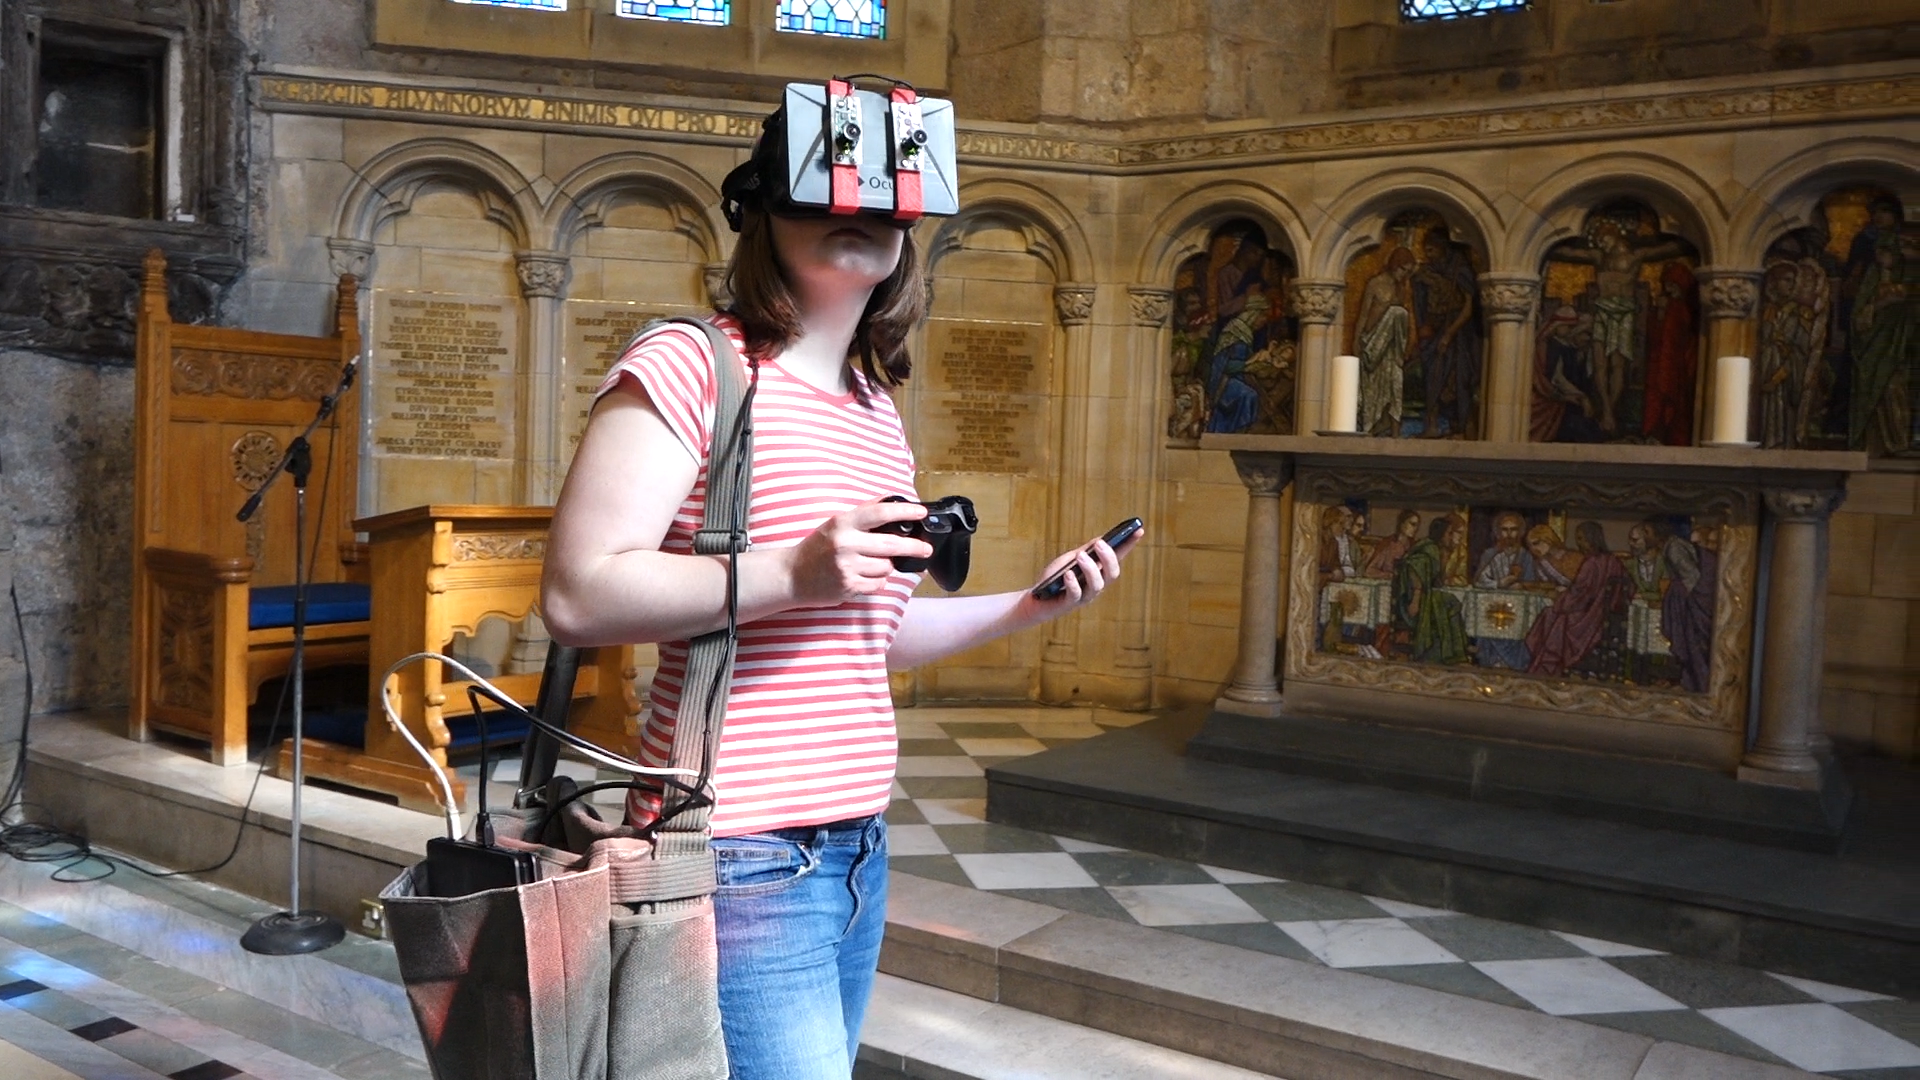
\includegraphics[width=\linewidth]{participant-f.png}
		\caption{Participant using Mirrorshades in a user study at St Salvator's chapel.}
		\label{participant-f.png}
	\end{center}
\end{figure}

\begin{figure}[ht]
	\begin{center}
		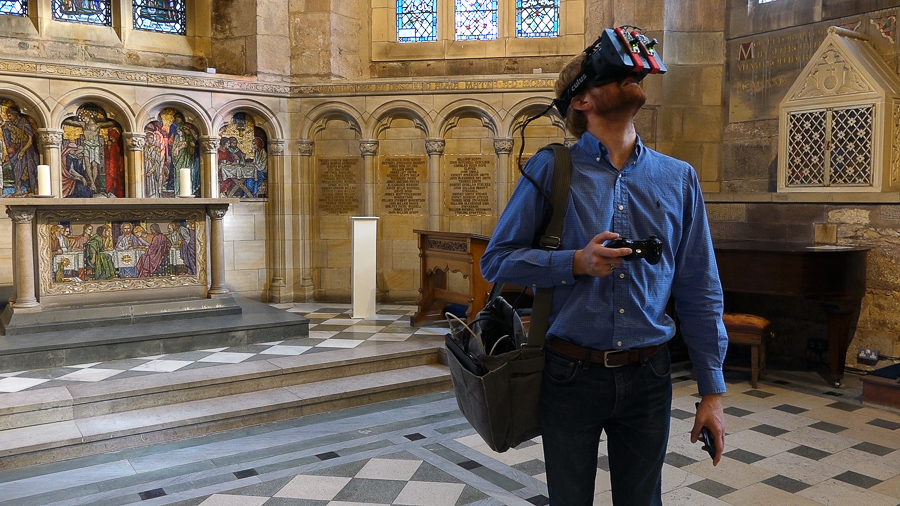
\includegraphics[width=\linewidth]{participant-m.png}
		\caption{Participant using Mirrorshades in a user study at St Salvator's chapel.}
		\label{participant-m.png}
	\end{center}
\end{figure}

%=========================================================================================================

\section{Stage 1 - PR for Virtual Heritage}

Previously when immersive VR has been employed in virtual heritage scenarios, it has predominantly been implemented as CAVE experiences~\cite{Roussou2002}. Visitors to a museum or visitor centre will be offered the opportunity to step into a CAVE, possibly donning shutter glasses or similar apparatus to enable a stereoscopic 3D effect, to experience a VR reconstruction of a location, its contents \& actors. Some of these CAVE installations have featured physical control interfaces such as joystick \& 3D mouse~\cite{cabral:x3dexperience} \& haptic interfaces~\cite{Christou2006}, while others have tracked user movement, whether head only or full body  gestures (such as in figure \ref{VTTP_projection.png}). In common among these CAVE experiences is the fact that the VR content they present is experienced with a disconnect to the RW site that it pertains to, as the CAVE itself immerses users in VR visuals \& does not permit them to see any of their RW surroundings, comparable to the experience of weareing a VR HMD without see-through video functionality. Furthermore, the physical size of the CAVE limits the amount in any particular direction that a user can physically move, even if movement is encouraged due to its use as a control methodology. This introduces both temporal \& spatial separation between a user's experiences of the VR content \& the corresponding RW environment.

With the promise of high performance VR HMDs at a consumer price point on the horizon, thanks largely to the rejuvenation in the field effected by Oculus, their use at cultural heritage sites for achieving similar experiences to previous CAVE installations is becoming more plausible \& brings with it certain benefits such as a reduction in the physical space required at the site for the installation. The OVW group's experience with presenting both experts \& interested amateurs, young \& old, with virtual heritage content via Oculus HMDs (both DK1 \& DK2, see section \ref{virtual-heritage-at-st-andrews}) has been very promising. These interactions have taken place in scenarios similar to those of existing CAVE scenarios; the user remains physically stationary \& uses a controller or gestures to move their virtual presence throughout the VR environment, whilst unable to observe their RW environment due to the nature of the HMD isolating them from RW visual stimuli.

In this first stage of the evaluation a comparison is made of this `traditional' style of interacting with VR content at a cultural heritage site wherein VR is experienced in isolation from RW, with both temporal \& spatial separation, against the `new' style afforded by the Mirrorshades PR platform, in which VR can be experienced in tandem with RW by allowing the user to move around their RW environment \& transition at any time into seeing the VR environment from the equivalent vantage point. Participants in this stage of the evaluation thus completed two scenarios wherein they interact with the RW St Salvator's chapel \& its corresponding VR reconstruction;

\begin{enumerate}
	\item \textbf{Traditional scenario} - Participants experience the RW \& VR chapels separately. They navigate the VR chapel from a stationary position, as VR has traditionally been employed at cultural heritage sites via CAVE installations \& by the OVW group with Oculus HMDs, using the Xbox controller to move around the VR environment observed via the DK1, with the DK1 obscuring their view of the RW chapel around them. Subsequently, they navigate the RW chapel without the DK1 or any associated equipment.
	\item \textbf{PR scenario} - Participants experience the RW \& VR chapels in tandem using the Mirrorshades platform. They wear the DK1, holding the Xbox controller in their right hand \& the smartphone in their left, with the laptop \& control box bundle in a satchel worn over one shoulder. Pressing \& holding a button on the Xbox controller triggers a transition from RW visual stimuli to VR visual displayed by the DK1.
\end{enumerate}

%=========================================================================================================

\subsection{Design of the Scenarios}

The scenarios were intended to mimic the style of exploration \& interaction that visitors to the chapel display, after observing the behaviour of such visitors on several occasions. From these observations, a common pattern of behaviour emerged: visitors enter the chapel from the North/West corner then proceed to walk Eastwards along the nave, pausing to look around after passing through the rood screen, before continuing along the nave toward the altar. They then pause in front of the altar upon reaching the end of the pews \& then walk North toward the tomb where they pause again to inspect it. Participants in this first stage of the evaluation process were instructed to imagine that they were performing a similar visit to the chapel \& to follow a similar path, pausing after the rood screen, at the end of the pews \& in front of the tomb to look around their environment(s) in more detail, however they were encouraged to stop \& look around at any times/positions that they wished \& not to feel restricted to the described path \& locations - the intent of the scenario was to encourage a natural style of exploration despite the unusual situation of making use of bulky VR hardware, rather than to restrict them to an `on rails' experience. Participants were shown the map included as figure \ref{chapel-path} (North upwards) to help visualise the scenario.

\begin{figure}[h]
	\begin{center}
		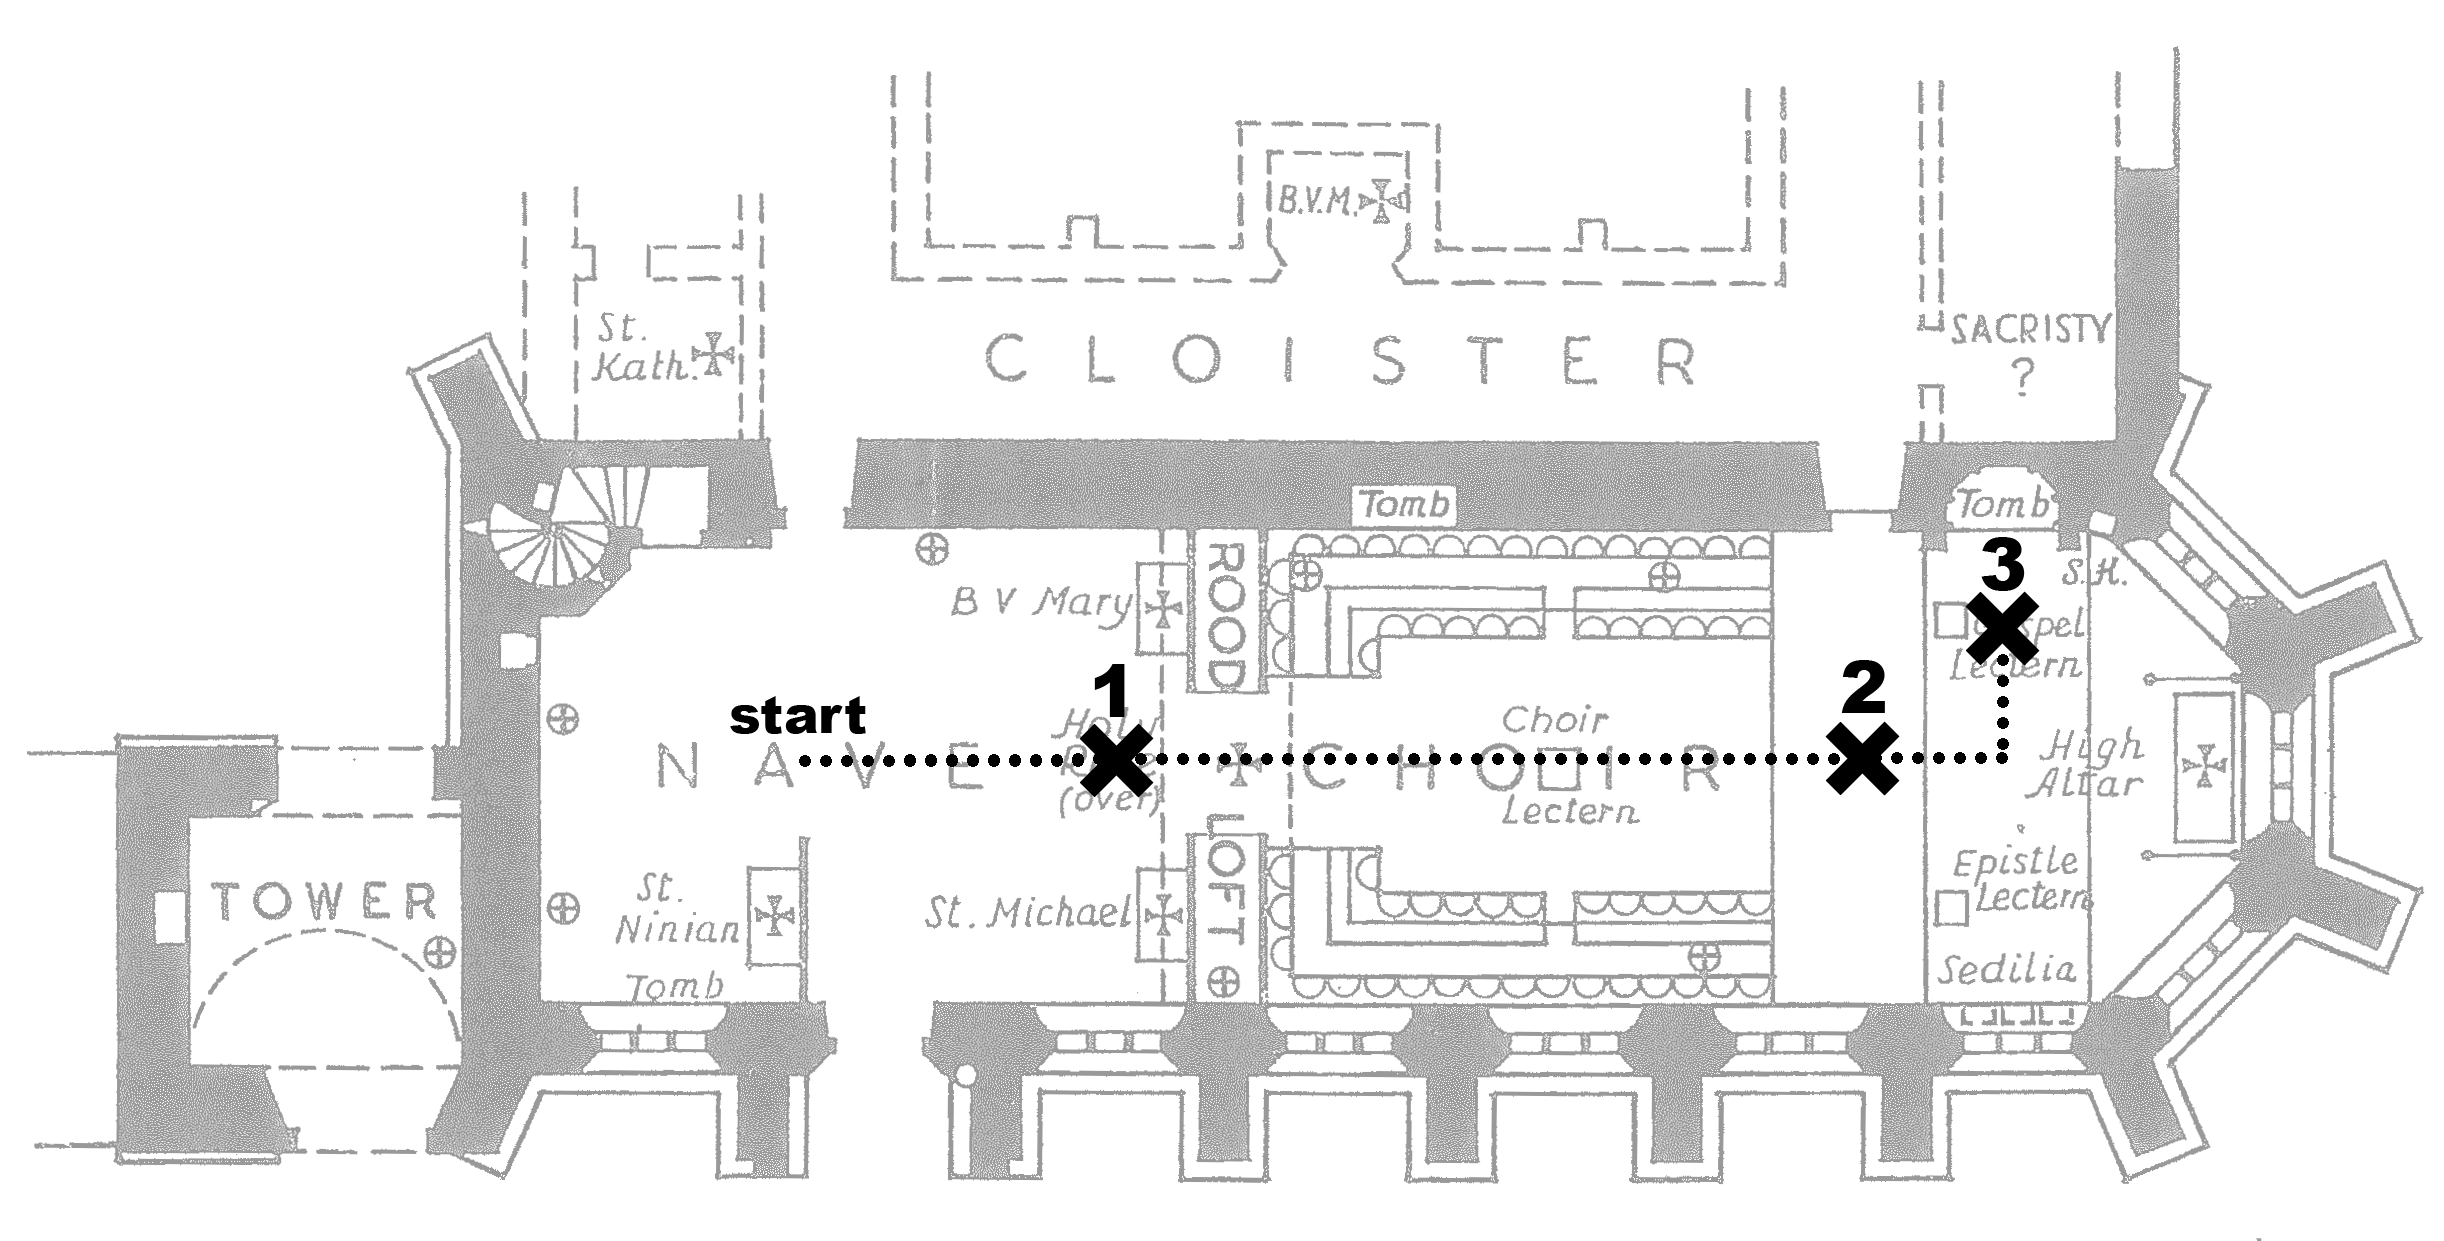
\includegraphics[width=.6\linewidth]{chapel-path.png}
		\caption{The path \& positions within the chapel that participants are instructed to attend to.}
		\label{chapel-path}
	\end{center}
\end{figure}

In the traditional scenario participants interacted with the VR chapel using the DK1 \& Xbox controller while seated. After completing the path in the VR chapel, they removed the DK1 \& walked the same path in the RW chapel. This behaviour alludes to how VR has previously been applied to cultural heritage sites such as St Salvator's chapel, wherein visitors would have the opportunity to experience a CAVE or stationary HMD based reconstruction of the site either before or after having explored the RW site. In the PR scenario participants wore the DK1, held the Xbox controller in their right hand \& the smartphone in their left, with the laptop \& control box bundle in a satchel worn over a shoulder (see figures \ref{participant-f.png} \& \ref{participant-m.png}). They then walked the same path, but this time with the ability to transition at any time between viewing the RW chapel \& the VR chapel from the equivalent vantage point.

In the PR scenario, participants had access to a single transition style, the transition with linear interpolation (see section \ref{transition-with-linear-interpolation}), triggered by pressing \& holding the \texttt{A} button on the Xbox controller. As mentioned in section \ref{initial-testing}, this transition emerged as the `favourite' during initial tests within the OVW group. As such, it was chosen as the only transition style for the PR scenario in this first stage of evaluation wherein the focus of the investigation was upon comparing the PR scenario to the traditional scenario experience \& not upon gleaning details of the merits \& drawbacks exhibited by different PR implementations. The default view on the DK1's screen was 100\% RW with the transition causing a change to 100\% VR, a situation visualised upon the combined model in figure \ref{focus-locus-sensus-with-virtuality-continuum-with-transition}.

Before taking part in the two scenarios, participants were given the opportunity to familiarise themselves with the DK1 by spending a few minutes interacting with Oculus' `Tuscany' demo\footnote{\url{https://share.oculus.com/app/oculus-tuscany-demo}}. This demo was developed by Oculus themselves \& is distributed with the Rift Unity integration package. It represented at the time a very polished \& stable DK1 experience, ideal for introducing inexperienced users to HMD based VR. It was thus used to give participants an opportunity to acclimatize to the Rift, in order to reduce skewing their subsequent experiences with the St Salvator's chapel model due to drastically different levels of familiarity with the DK1 between the two scenarios.

%=========================================================================================================

\subsection{Evaluation Techniques}

The comparison of the traditional scenario against the PR scenario was facilitated by the collection of a variety of both qualitative \& quantitative data. All participants completed a pre-task questionnaire which provided calibration for latter data by enquiring about age, gender identity, previous experience with VR HMDs \& whether they had previously visited St Salvtor's chapel, both RW \& VR (the RW chapel is open to the public \& a version of the VR reconstruction is publicly accessible via the OVW group's OpenSim grid\footnote{\url{openvirtualworlds.org}}). The System Usability Scale (SUS)~\cite{Brooke1996} was used to provide a basic comparison between the usability of the two scenarios, while a 12-item Likert-type questionnaire (included as appendix \ref{appendix-12-item-likert-type-questionnaire-stage-1}) was used to collect opinions on more specific aspects of the experience of both scenarios. At the end of the session, after completing both scenarios, participants were engaged in a short structured interview (prompts included as appendix \ref{appendix-interview-questions-stage-1}) in order to allow them to elaborate upon their experience in a more free form manner. Finally, in addition to the DK1 visuals being recorded via ShadowPlay, log data were collected during both scenarios, capturing the information detailed in table \ref{logdatatable} to file for each frame rendered to the DK1's screen.

\begin{center}
\begin{longtable}{| l | p{8cm} |}

\hline

\textbf{Field} & \textbf{Description} \\

\hline

\texttt{<frame number>} & Incremented with each frame pushed to the DK1, starting at 0 when the Unity application is run. \\

\hline

\texttt{<timestamp>} & According to the laptop's internal clock. \\

\hline

\texttt{<original\_position>} & The position as a Unity \texttt{Vector3} where the participant begins the experiment (as reported by IndoorAtlas). \\

\hline

\texttt{<position>} & The position as a Unity \texttt{Vector3} where the participant is on this frame (as reported by IndoorAtlas). \\

\hline

\texttt{<delta\_x>} \& \texttt{<delta\_z>} & The difference in the \texttt{x} \& \texttt{z} axes between \texttt{<original\_position>} \& \texttt{<position>} on this frame. Change in elevation (\texttt{y} axis) is not recorded, as IndoorAtlas does not provide elevation data \& the area of St Salvator's chapel used throughout the studies is level. \\

\hline

\texttt{<left\_rotation>} \& \texttt{<right\_rotation>} & The orientations as Unity \texttt{Quaternion} of the two Unity camera game objects. The orientation of these Unity objects is tied to the orientation of the DK1, so these values represent the orientation of the participant's head on each frame. \\

\hline

\texttt{<base\_oapcity>} & The maximum opacity of the game objects upon which the camera feeds are rendered. This is how reduced maximum opacity (see section \ref{subsub-baseopacity}) is implemented (by setting this field to a value \textless 1). \\

\hline

\texttt{<left\_opacity>} \& \texttt{<right\_opacity>} & The opacity on this frame of the game objects upon which the camera feeds are rendered. \\

\hline

\texttt{<auto\_tick>} & Whether a periodic switch is in progress (see section \ref{subsub-periodic}). \\

\hline

\texttt{<auto\_duration>} \& \texttt{<auto\_spacing>} & The interval \& duration values of the periodic hard switching (if applicable). \\

\hline

\texttt{<framerate>} & An estimate of the current frame rate (frames per second). \\

\hline

\texttt{<A\_button>}, \texttt{<B\_button>} \& \texttt{<right\_trigger>} & The current values of these inputs on the Xbox controller. For the \texttt{A} \& \texttt{B} buttons this is binary, either pressed or not, while for the trigger it is a numeric value representing the amount that the trigger is being depressed. \\

\hline
\caption{Log data captured during Mirrorshades evaluations.}
\label{logdatatable}
\end{longtable}
\end{center}

%=========================================================================================================

%\subsection{Process}

%The stage 1 investigations took place as follows;

%\begin{enumerate}
%	\item Participants completed the pre-task questionnaire.
	
%	\item Participants were given the opportunity to familiarise themselves with the DK1 by spending a few minutes interacting with Oculus' `Tuscany' demo\footnote{\url{https://share.oculus.com/app/oculus-tuscany-demo}}. This demo was developed by Oculus themselves \& is distributed with the Rift Unity integration package. It represented at the time a very polished \& stable DK1 experience, ideal for introducing inexperienced users to HMD based VR. It was thus used to give participants an opportunity to acclimatize to the Rift, in order to reduce skewing their subsequent experiences with the St Salvator's chapel model due to drastically different levels of familiarity with the DK1 between the two scenarios.
	
%	\item Participants completed the traditional scenario.
	
%	\item Participants completed the SUS questionnaire \& the 12-item Likert-type questionnaire for their experience with the traditional scenario.
	
%	\item Participants completed the PR scenario.
	
%	\item Participants completed the SUS questionnaire \& the 12-item Likert-type questionnaire for the PR scenario.
	
%	\item Participants are engaged in a short structured interview.
%\end{enumerate}

%=========================================================================================================

\subsection{Hypotheses}
\label{stage1hypotheses}
This first stage of evaluation was designed to ascertain whether applying mobile PR to a cultural heritage scenario results in an improvement in participant engagement with \& understanding of the relationships between the RW \& VR environments, compared to a traditional virtual heritage scenario. Such improvements were expected to result from addressing the problems of spatial \& temporal separation inherent with the traditional scenario by imparting upon the participant the ability to transition at will between equivalent vantage points within the RW \& VR environments.

Overall participants were expected to report that the PR scenario did allow them to better compare \& contrast the RW \& VR environments, identify differences between the RW \& VR environments \& gain a better understanding of how the RW \& VR environments relate to each other. However it was also expected that some participants would report that having to `split' their attention between the two environments in the PR scenario led to lessened engagement \& understanding \& that the visual quality of the RW view through the cameras led to them preferring the traditional scenario.

It was expected that the cumbersome nature of the PR scenario in terms of the hardware that needed to be carried by the participant \& the reduced quality of viewing the RW environment via the cameras would have a noticeable effect upon participants' movement (both in terms of their position \& the orientation of their head) in the PR scenario compared to the VR section of the traditional scenario, most likely a restriction. The cumbersome nature of the hardware was also expected to impact SUS scores, with the PR scenario averaging lower than the traditional scenario. Participants who were able to overcome this cumbersomeness were expected to respond more favourably to the PR scenario than those who could not.

The 12-item Likert-type questionnaire was expected to reveal several distinctions. In particular;
\begin{itemize}
	\item Participants will find it easier to compare \& contrast RW \& VR environments in the PR scenario than in the traditional scenario (q2)
	\item Participants will experience a greater  sense of `being there' in the VR environment in the PR scenario than in the traditional scenario, due to physical movement/embodiment~\cite{Groten2011} (q4)
	\begin{itemize}
		\item Furthermore, participants will have a greater sense of `being in the past' in the PR scenario than in the traditional scenario (q7)
	\end{itemize}
	\item Participants will maintain greater awareness of both RW \& VR environments in the PR scenario than in the traditional scenario (q5)
	\item Participants will gain a better understanding of what the chapel was like in the past in the PR scenario than in the traditional scenario (q12)
\end{itemize}

In addition to substantiating or refuting questionnaire results \& interview responses, the log data themselves were expected to provide insight into relationships between several aspects of the traditional \& PR scenarios, such as;
\begin{itemize}
	\item Head movement (pitch \& yaw) will be more restricted in the PR scenario compared to the VR section of the traditional scenario
	\item Participants will display an aversion to looking around (even at RW) when moving in the PR scenario
\end{itemize}

Interview transcripts were expected to lend support to the following assumptions;
\begin{itemize}
	\item the PR scenario makes it easier to spot differences between RW \& VR than the traditional scenario
	\item the PR scenario reveals differences that the traditional scenario didn't
	\item the traditional scenario does not reveal differences that the PR scenario didn't
	\item the PR scenario is preferred \& is user-reported as 'more engaging' than the traditional scenario
\end{itemize}

Assessing the severity of these issues through this first stage of evaluation is critical such that future PR implementations can be informed in order to allow them to achieve a quality of experience sufficient that participants do not feel that the drawbacks outweigh the benefits. For application of PR to virtual heritage to be a success, users must not feel restricted from performing transitions due to their jarring nature, or prefer a traditional virtual heritage experience due to the superior visual acuity of unmediated RW stimuli compared to mediated RW stimuli in the PR scenario.

%=========================================================================================================

\section{Stage 1 Results}

A total of 6 participants completed the stage 1 investigation;
\begin{itemize}
	\item Age ranged from 21 to 26, with a mean of 23.3 \& a standard deviation of 1.86
	\item 3x identified as male \& 3x as female
	\item All reported previous experience with a games console controller
	\item 1x reported previous experience with a HMD
	\item 2x reported having previously visited the chapel
	\item None had previously experienced the virtual chapel
\end{itemize}

%=========================================================================================================

\subsection{SUS}
As expected, the PR scenario scored lower on SUS than the traditional scenario (see figure \ref{sus.png}), but not drastically so.

\TwoFig{1/sus.png}{SUS results for stage 1.}{sus.png}
       {1/post_task_questionnaire_boxplot.png}{Likert-type questionnaire results.}{post_task_questionnaire_boxplot.png}

%=========================================================================================================

\subsection{Likert-type Questionnaires}

One participant did not complete the Likert-type questionnaires. Coincidentally this participant was also the only one to have reported previous experience with a HMD in the pre-task questionnaire, so the Likert-type questionnaire responses wholly represent participants with no prior HMD experience. With the resurgence of interest in HMD based VR in recent years, the number of developers \& enthusiasts with HMD experience is climbing. However until the first commercial VR HMDs are released \& begin to permeate gaming \& media consumption audiences the situation captured by these questionnaire results, where all visitors to a cultural heritage site had no previous HMD experience, should be considered representative of the general public. When considering the responses to the Likert-type questionnaires (see figure \ref{post_task_questionnaire_boxplot.png}) for the first stage participants several observations can be made.

\begin{itemize}
	\item Participants enjoyed the PR scenario more than the traditional scenario (q1)
	\item Participants found it easier to compare features from past \& present in the PR scenario (q2)
	\item Perceived motion sickness/dizziness was not noticeably different between the two scenarios (q3)
	\item There was a greater sense of `being there' in the VR environment in the PR scenario (q4)
	\item There was a greater awareness of both environments in the PR scenario (q5)
	\item Participants found the PR scenario a more rewarding way to explore the chapel (q6)
	\item Participants had a greater sense of being in the past in the PR scenario (q7)
	\item Both scenarios scored fairly low for participants thinking they would have preferred a conventional monitor (q8)
	\item The PR scenario changed participants’ understanding of the chapel more than the traditional scenario (q9)
	\item Both scenarios scored equally low for participants’ thinking they did not notice differences between RW \& VR (q10)
	\item The visual quality of the headset was perceived as being worse in the mobile scenario (q11). Whilst the visual quality of the VR visuals was identical in both scenarios, this result is presumably because during the PR scenario the participants were viewing the RW environment upon the DK1's screen via the cameras, with much lower visual acuity than in the traditional scenario where they observed the RW environment unmediated.
	\item Participants felt that they better understood what the chapel was like in the past after the PR scenario, compared to the traditional scenario (q12)
\end{itemize}

These results largely confirm the hypotheses from section \ref{stage1hypotheses}. It is also worth noting that although the PR scenario scored lower than the traditional scenario in SUS, both scenarios scored highly in question 2 (\textit{``It was easy to compare features from the past \& the present''}) \& low in question 8 (\textit{``I would have preferred a conventional computer monitor''}).

%=========================================================================================================

\subsection{Interview Transcripts}

Studying the structured interviews that took place after participants had completed both scenarios (interviews were recorded \& subsequently transcribed) provided a wealth of qualitative feedback about the stage 1 investigation.

All participants said that the PR scenario was (much) more engaging than the traditional scenario, even though 2x participants said that they preferred the traditional scenario. Of those that said they preferred the traditional scenario, one did not find it comfortable to walk while wearing the DK1 \& the other reported gaining a better understanding of the past from the traditional scenario. The participant who found it uncomfortable to walk while wearing the DK1 was notably taller than all of the other participants in this stage. This is worth mentioning as the `height' of the virtual cameras in the VR reconstruction was fixed with reference to the UK average height of 5 feet 9 inches \& was not changed to account for different participant heights, as this would have required a lengthy calibration phase for each \& every participant. Thus for a participant of average height, the discrepancy between their RW viewpoint \& their VR viewpoint was minimal, however for a particularly short or tall participant this discrepancy would have been much worse \& may have contributed to the discomfort of walking with the DK1 as each transition between RW \& VR would have resulted in a perceptible shift in height. Those that said that they preferred the PR scenario alluded to the immediacy of comparison between RW \& VR afforded by it as a contributing factor.

Twice as many participants reported that the PR scenario made it easier to spot differences between RW \& VR as reported that the traditional scenario made it easier, with 4 out of 6 participants reporting noticing differences between RW \& VR in the PR scenario that they did not notice in the traditional scenario. In particular, the different position of the rood screen was mentioned by several participants \& one participant was able to list multiple differences that s/he had spotted in the PR scenario that they had not noticed in the traditional scenario. One participant directly mentioned then confirmed that immediacy of comparison between RW \& VR was the enabler of spotting more differences, another mentioned that with the traditional scenario it was not clear that you were \textit{``trying to look into the past''} but in the PR scenario it was obvious because \textit{``you can see the differences''}, while another directly said that s/he preferred the PR scenario because \textit{``it was easier to compare \& contrast between the real world \& the virtual one''}.

The quality of the cameras was mentioned as a possible detractor by one of the participants who answered that the traditional scenario made it easier to spot differences between RW \& VR, with another participant specifically mentioning that a higher \textit{``resolution''} was needed.

The one participant to report experiencing motion sickness elaborated that it was worse when using the DK1 in the traditional scenario than when walking with the DK1 in the PR scenario, because \textit{``sitting down \& moving around feels weird''} (a reference to moving throughout the VR environment using the Xbox controller whilst physically stationary sitting on a chair). This observation alludes to the idea of physical embodiment/movement improving a VR experience, by demonstrating the opposite position of restricted movement \& a lack of matching embodiment worsening the VR experience.

With regards to movement in the PR scenario, the accuracy \& especially the lag of the indoor positioning was cited by one participant as needing work, because it \textit{``caught me off guard twice''}. From watching the ShadowPlay recorded videos from the PR scenario, it is clear that in many cases the participants would trigger a transition to VR visual stimuli only to find that their VR position had not yet `caught up' with their RW position.

%=========================================================================================================

\subsection{Log Data}

For the traditional scenario log data were recorded while each participant was engaging with the VR chapel, in a seated position \& using the Xbox controller to navigate the VR environment. For the PR scenario log data were recorded throughout the whole scenario, such that data are available for both the periods in which participants were observing the RW chapel via the DK1 \& cameras in addition to the periods in which participants were observing the VR chapel. As such, several comparisons can be made between these data. Within the PR scenario, comparisons can be made between the periods that participants were observing RW \& the periods that participants were observing VR. Between the traditional scenario \& the PR scenario, comparisons can be made between the VR section of the traditional scenario \& the periods that participants were observing VR in the PR scenario. Log data were not captured for participant 2, nor were they captured for the traditional scenario for participant 5.

\subsubsection{Comparing traditional \& PR scenarios}

When looking at either scenario's data (the VR section of the traditional scenario \& both RW \& VR periods of the PR scenario) it is immediately evident that participants looked to their sides \& turned their heads horizontally (yaw) far more than they looked above \& beneath themselves by tilting their heads vertically (pitch). This relationship is shown in figures \ref{1_pitch_yaw_2up.png}, \ref{4_pitch_yaw_2up.png} \& \ref{6_pitch_yaw_2up.png}, which show pitch \& yaw plotted against time for both the traditional scenario \& the PR scenario, for participants 1, 4 \& 6 respectively. With the traditional scenario on the left of each pair of plots \& the PR scenario on the right, the displacement of the blue line representing yaw is substantially greater in both than the displacement of the red line representing yaw.

\begin{figure}
	\begin{center}
	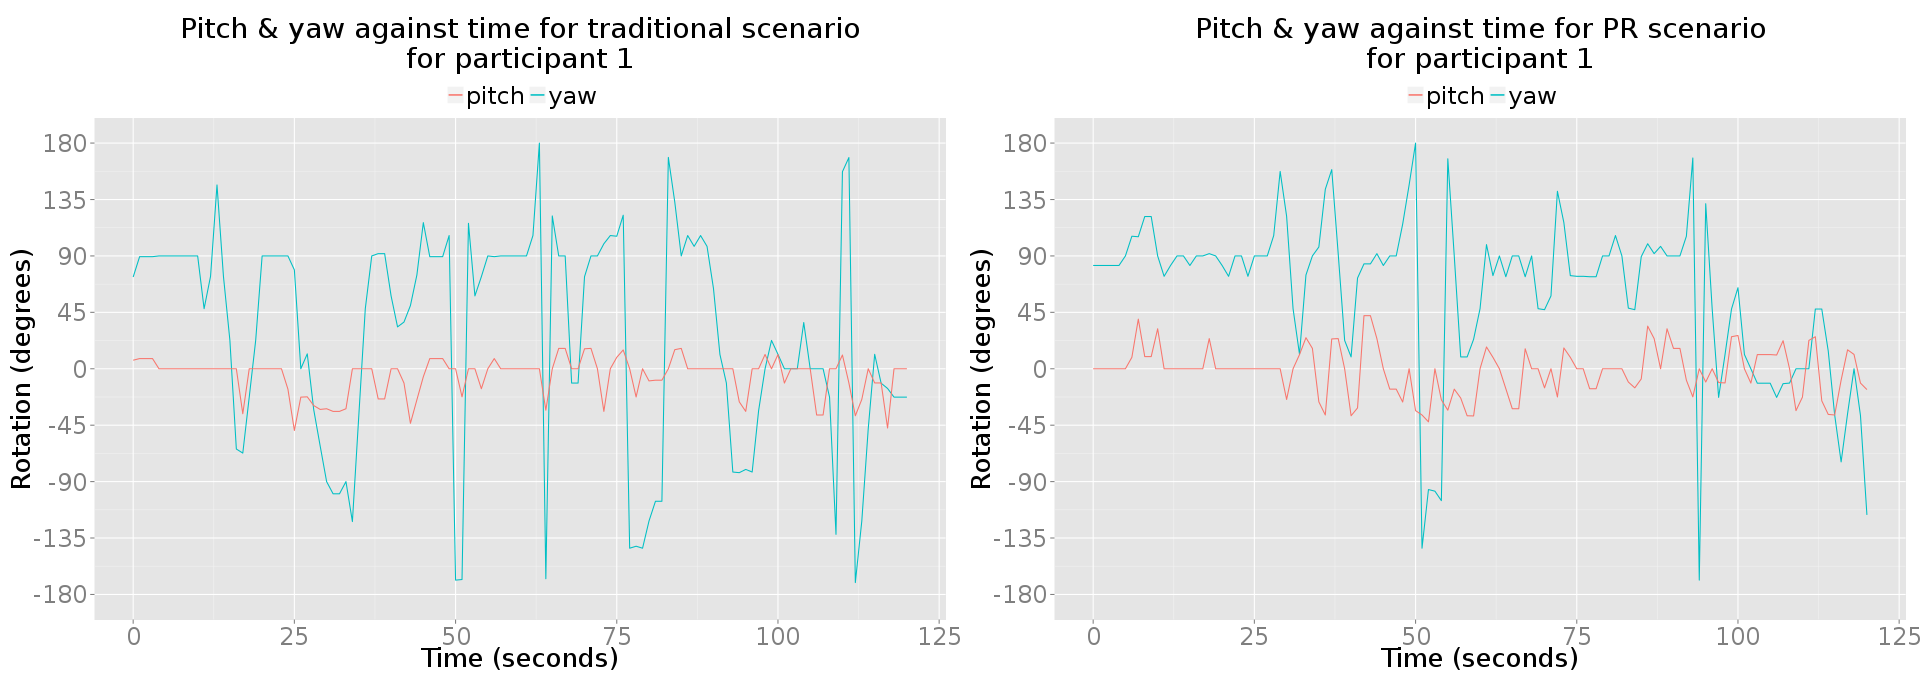
\includegraphics[width=\textwidth]{1/1_pitch_yaw_2up.png}
	\caption{Pitch \& yaw against time for participant 1 in traditional \& PR scenarios.}
	\label{1_pitch_yaw_2up.png}
	\end{center}
\end{figure}

\begin{figure}
	\begin{center}
	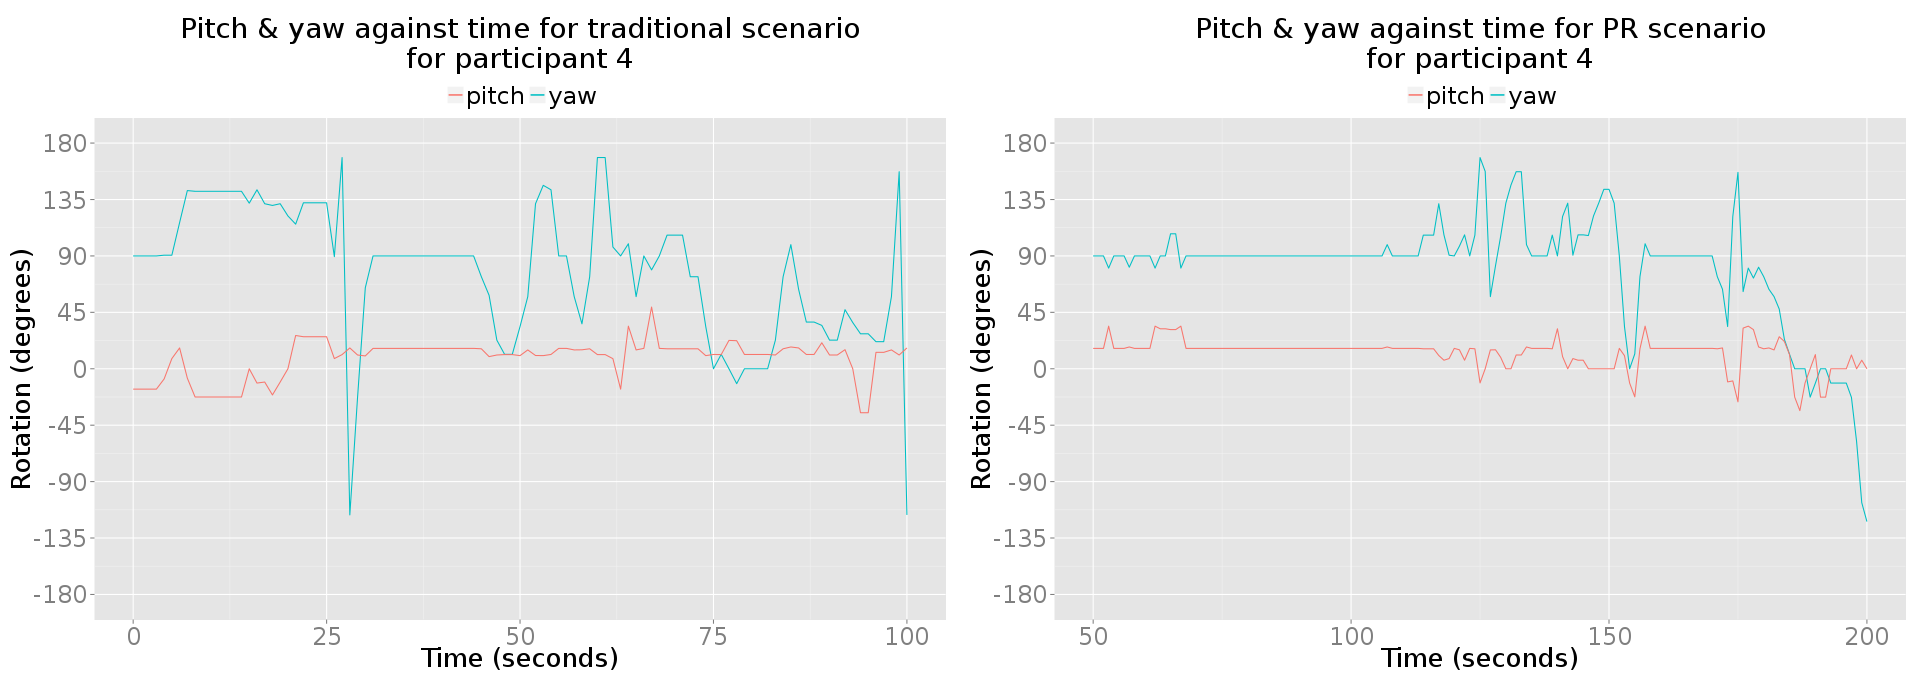
\includegraphics[width=\textwidth]{1/4_pitch_yaw_2up.png}
	\caption{Pitch \& yaw against time for participant 4 in traditional \& PR scenarios.}
	\label{4_pitch_yaw_2up.png}
	\end{center}
\end{figure}

\begin{figure}
	\begin{center}
	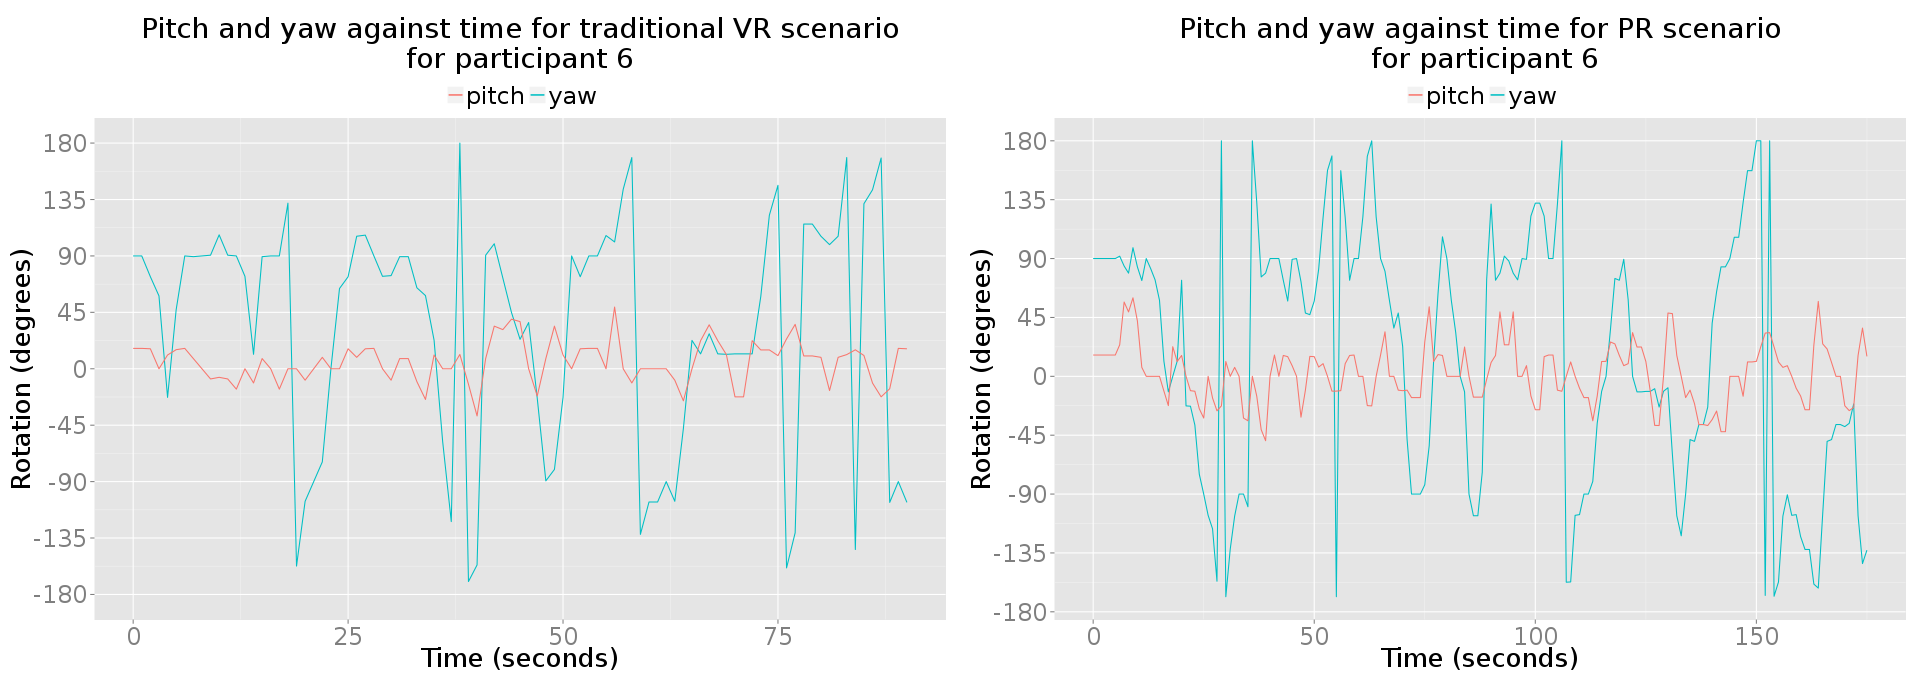
\includegraphics[width=\textwidth]{1/6_pitch_yaw_2up.png}
	\caption{Pitch \& yaw against time for participant 6 in traditional \& PR scenarios.}
	\label{6_pitch_yaw_2up.png}
	\end{center}
\end{figure}

This relationship is reflected calculating the standard deviation in pitch \& yaw across both scenarios, shown by table \ref{sdpitchyawtrad} for the traditional scenario \& table \ref{sdpitchyawpr} for the PR scenario. For every participant for which the data are available, the standard deviation in yaw is substantially higher than that in pitch. This relationship can largely be explained by the simple fact that there is more to observe in the chapel(s) at ground level than above eye level or upon the ground, however with the marked difference in the appearance of the chapel roof (stone in the VR reconstruction, wood in the RW chapel today) a smaller difference between pitch \& yaw variance might have been expected for both scenarios.

\begin{table}
\begin{center}
\begin{minipage}[t]{.47\linewidth}
\begin{center}
\begin{tabular}{|c|c|c|}
\hline

\textbf{Participant} & \textbf{Pitch (\textdegree)} & \textbf{Yaw (\textdegree)} \\

\hline

1 & 14.977 & 86.211 \\

\hline

3 & 16.684 & 60.545 \\

\hline

4 & 10.516 & 53.805 \\

\hline

5 & no data & no data \\

\hline

6 & 16.172 & 92.416 \\

\hline
\end{tabular}
\caption{Standard deviation in pitch \& yaw for traditional scenario.}
\label{sdpitchyawtrad}
\end{center}
\end{minipage}
%
\begin{minipage}[t]{.47\linewidth}
\begin{center}
\begin{tabular}{|c|c|c|}
\hline

\textbf{Participant} & \textbf{Pitch (\textdegree)} & \textbf{Yaw (\textdegree)} \\

\hline

1 & 19.186 & 63.427 \\

\hline

3 & 24.228 & 51.666 \\

\hline

4 & 11.723 & 44.526 \\

\hline

5 & 16.542 & 39.601 \\

\hline

6 & 21.999 & 97.122 \\

\hline
\end{tabular}
\caption{Standard deviation in pitch \& yaw for PR scenario (RW \& VR periods combined).}
\label{sdpitchyawpr}
\end{center}
\end{minipage}
\end{center}
\end{table}

%=====================

When studying plots of head pitch \& yaw against time aligned with plots of distance moved against time, some participants display an aversion to large head movements while moving. Considering participant 1 (figure \ref{1_4up.png}), they seem to have been quite comfortable looking around a lot even while moving in the traditional scenario, while in the PR scenario their large head movements are close to the periods in which their position was not changing as much\footnote{When looking at these plots it is important to appreciate that lag in the IndoorAtlas data results in a small lateral offset between the position data \& the head orientation data, as the latter is unaffected by the lag in the correct reporting \& `settling' of the former.}. When looking at the same data plotted for participant 3 however (figure \ref{3_4up.png}), it seems that they were reluctant to perform large head movements while moving in both scenarios, rather than just the PR scenario.

\begin{figure}
	\begin{center}
	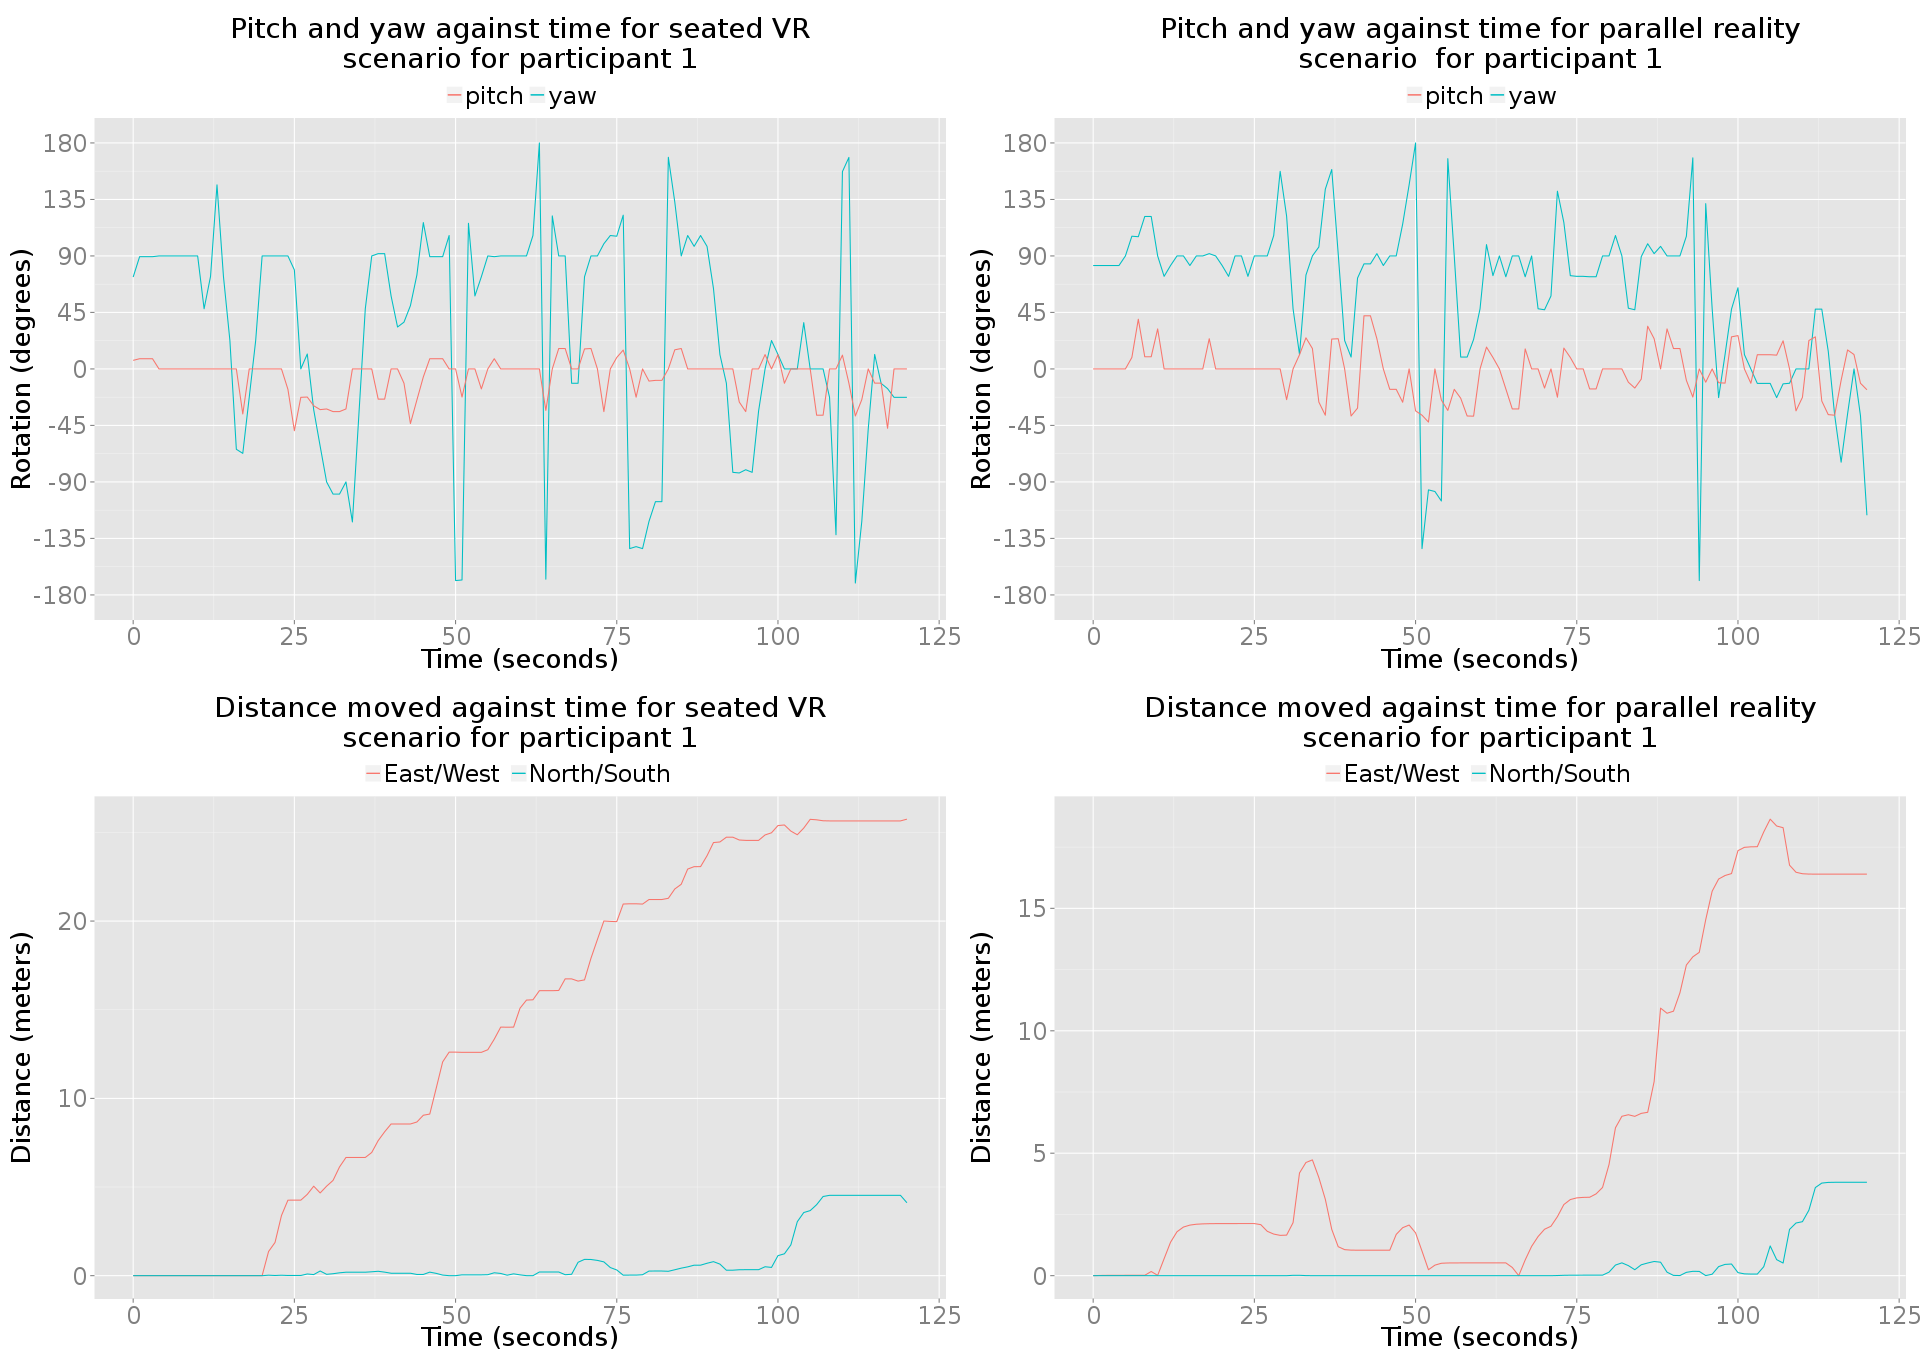
\includegraphics[width=\textwidth]{1/1_4up.png}
	\caption{Pitch \& yaw against time, aligned with distance moved against time, for participant 1 in both scenarios.}
	\label{1_4up.png}
	\end{center}
\end{figure}

\begin{figure}
	\begin{center}
	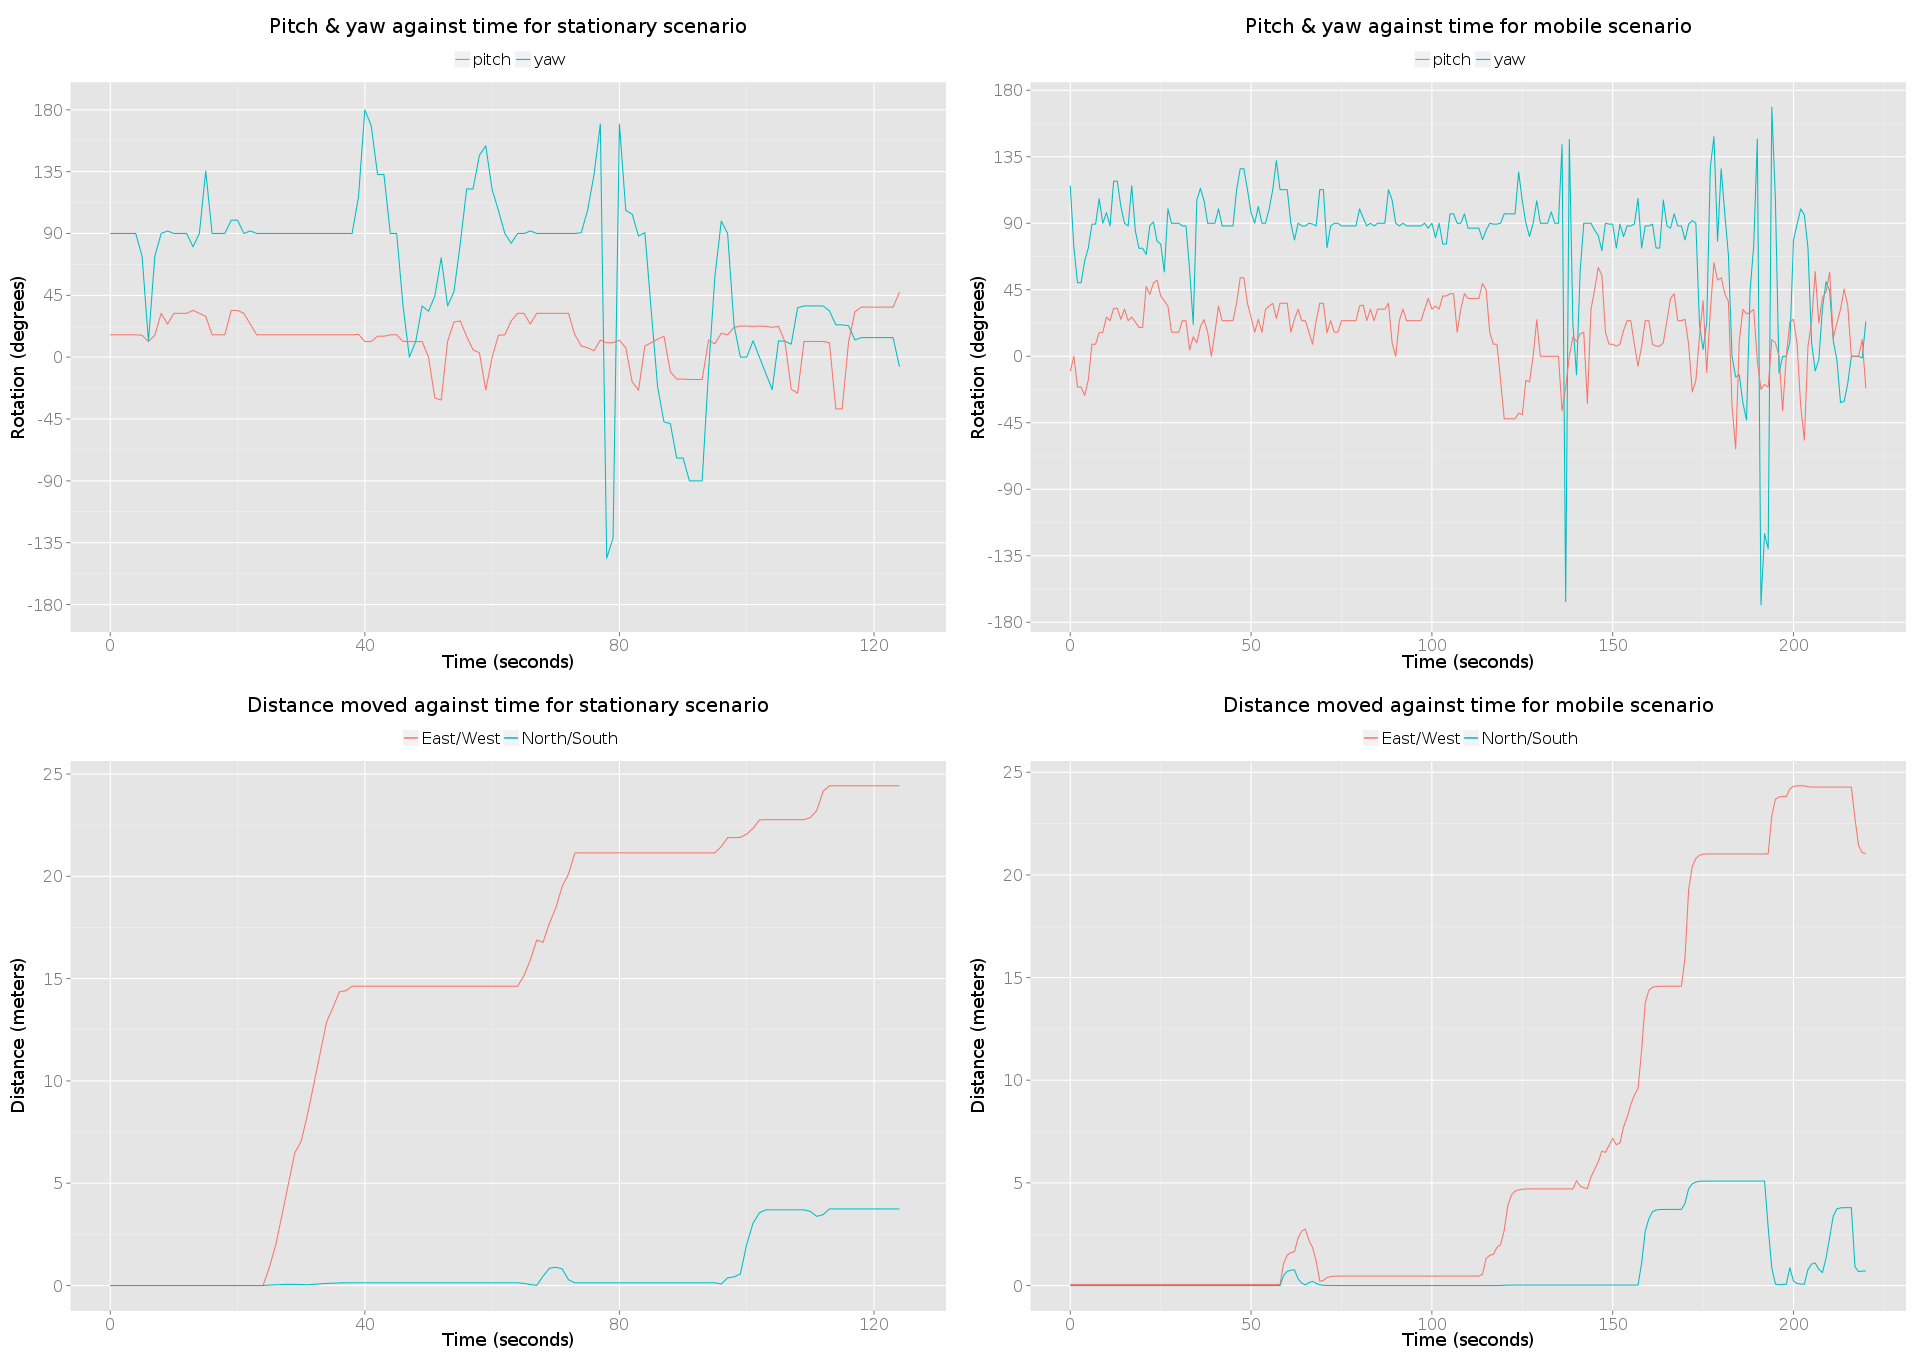
\includegraphics[width=\textwidth]{1/3_4up.png}
	\caption{Pitch \& yaw against time, aligned with distance moved against time, for participant 3 in both scenarios.}
	\label{3_4up.png}
	\end{center}
\end{figure}

Reluctance to changing head orientation when moving in the traditional scenario can be explained by something as simple as participant 1 having more experience with video games that present the user with a `first person' perspective in which movement \& looking direction are controlled independently. For somebody familiar with this style of control, it is second nature to use one control to change their position whilst simultaneously using another control to change the direction in which they are looking, however for those unfamiliar or inexperienced with such scenarios it is common to observe alternation between movement \& looking, something that the OVW group has observed in people interacting with our content at various demonstrations using keyboard \& mouse, Xbox controller \& other control methodologies. For first person shooter (FPS) video games, this is commonly achieved by using keyboard buttons to control movement while using a mouse to control looking direction. With the traditional scenario, the Xbox controller provides control over movement while the head tracker in the DK1 provides control over looking direction by tracking head orientation.

Reluctance to changing head orientation when moving in the PR scenario is most logically explained by participants feeling as though with the reduced visual acuity of their RW environment \& the discrepancy in position \& environmental objects of their VR environment that they needed to pay more conscious attention to their walking.

\subsubsection{Comparing RW \& VR periods within PR scenario}

When comparing pitch \& yaw data between the RW \& VR periods within the PR scenario, it is notable that for some participants there was more variance in the periods in which they were perceiving VR stimuli than in those in which they were perceiving RW stimuli, meaning that they turned their head more when looking at the VR environment than when looking at the RW environment. This is particularly evident when plotting these pitch \& yaw data against time with the RW/VR visuals indicated. Figure \ref{1_pitch_yaw.png} shows the pitch \& yaw data for participant 1 during the PR scenario, who prominently displayed this tendency toward greater head movement while viewing VR than RW. The coloured background of the plot indicates which environment the participant was perceiving at that time index; blue for RW \& green for VR. There is evident correlation to be seen between the most pronounced changes in yaw (red line) \& the periods that the participant was observing VR stimuli (green background).

\begin{figure}[h]
	\begin{center}
	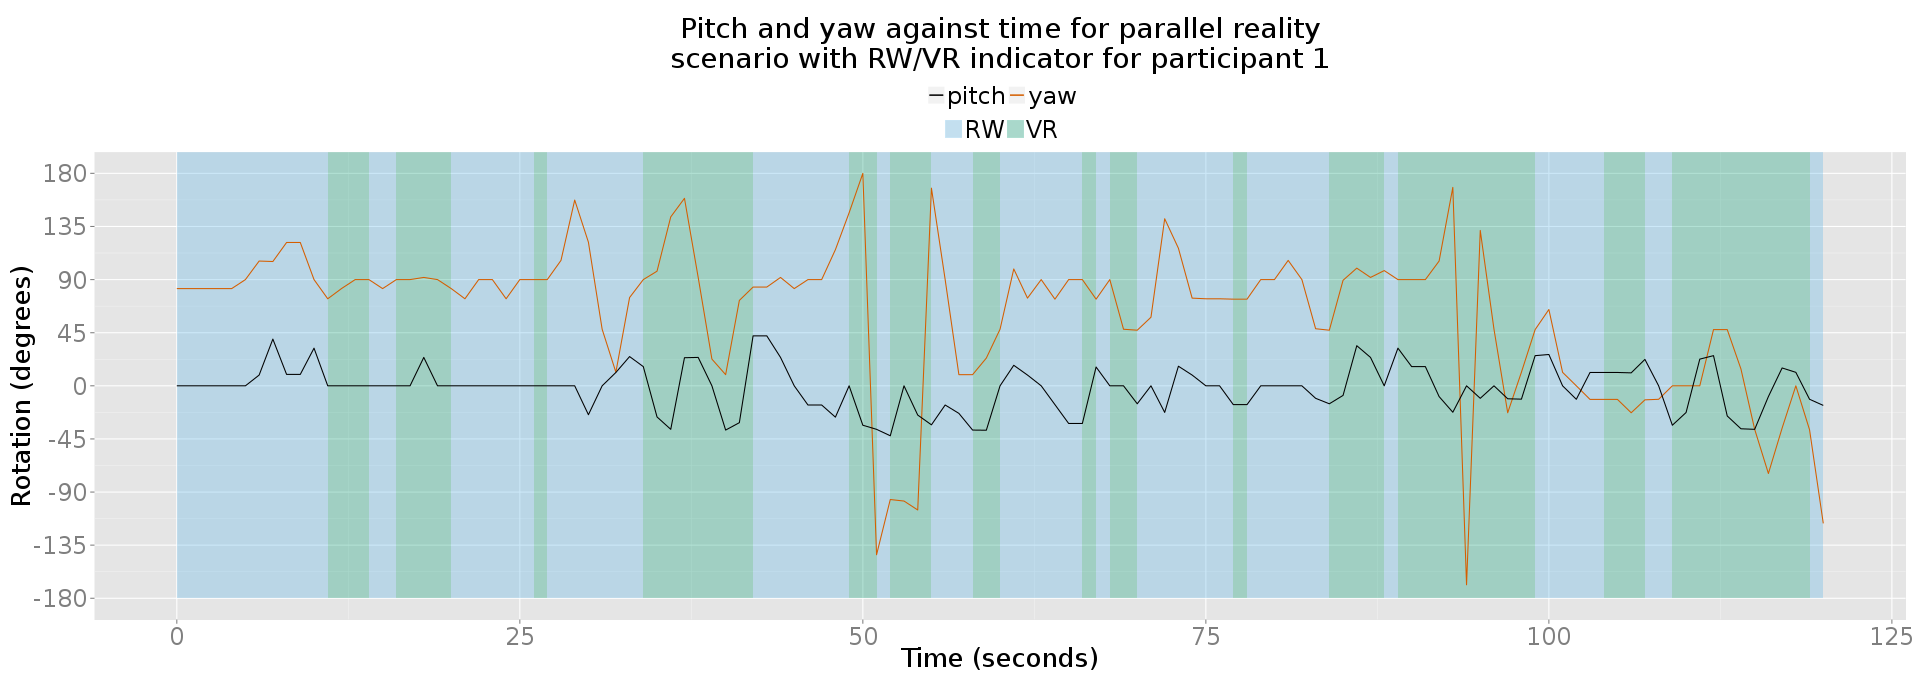
\includegraphics[width=\textwidth]{1/1_pitch_yaw.png}
	\caption{Pitch \& yaw against time for participant 1 in PR scenario, showing RW/VR periods.}
	\label{1_pitch_yaw.png}
	\end{center}
\end{figure}

As can be seen in figure \ref{3_pitch_yaw.png} this relationship is even more prevalent in the data from participant 3, while the data from participant 5 in figure \ref{5_pitch_yaw.png} still show the relationship but to a lesser extent.

\begin{figure}[h]
	\begin{center}
	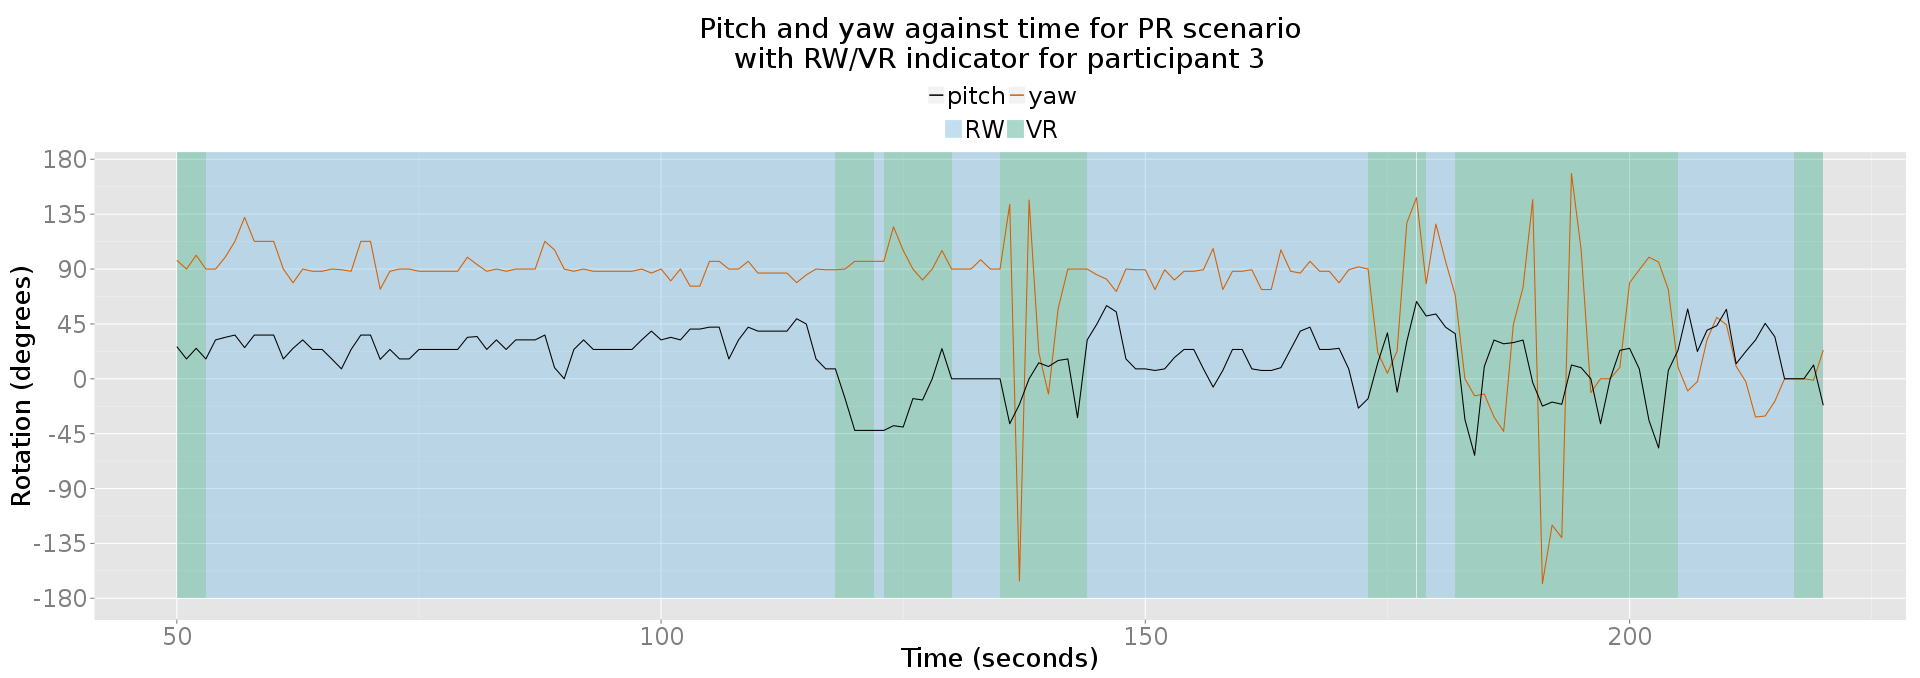
\includegraphics[width=\textwidth]{1/3_pitch_yaw.png}
	\caption{Pitch \& yaw against time for participant 3 in PR scenario, showing RW/VR periods.}
	\label{3_pitch_yaw.png}
	\end{center}
\end{figure}

\begin{figure}[h]
	\begin{center}
	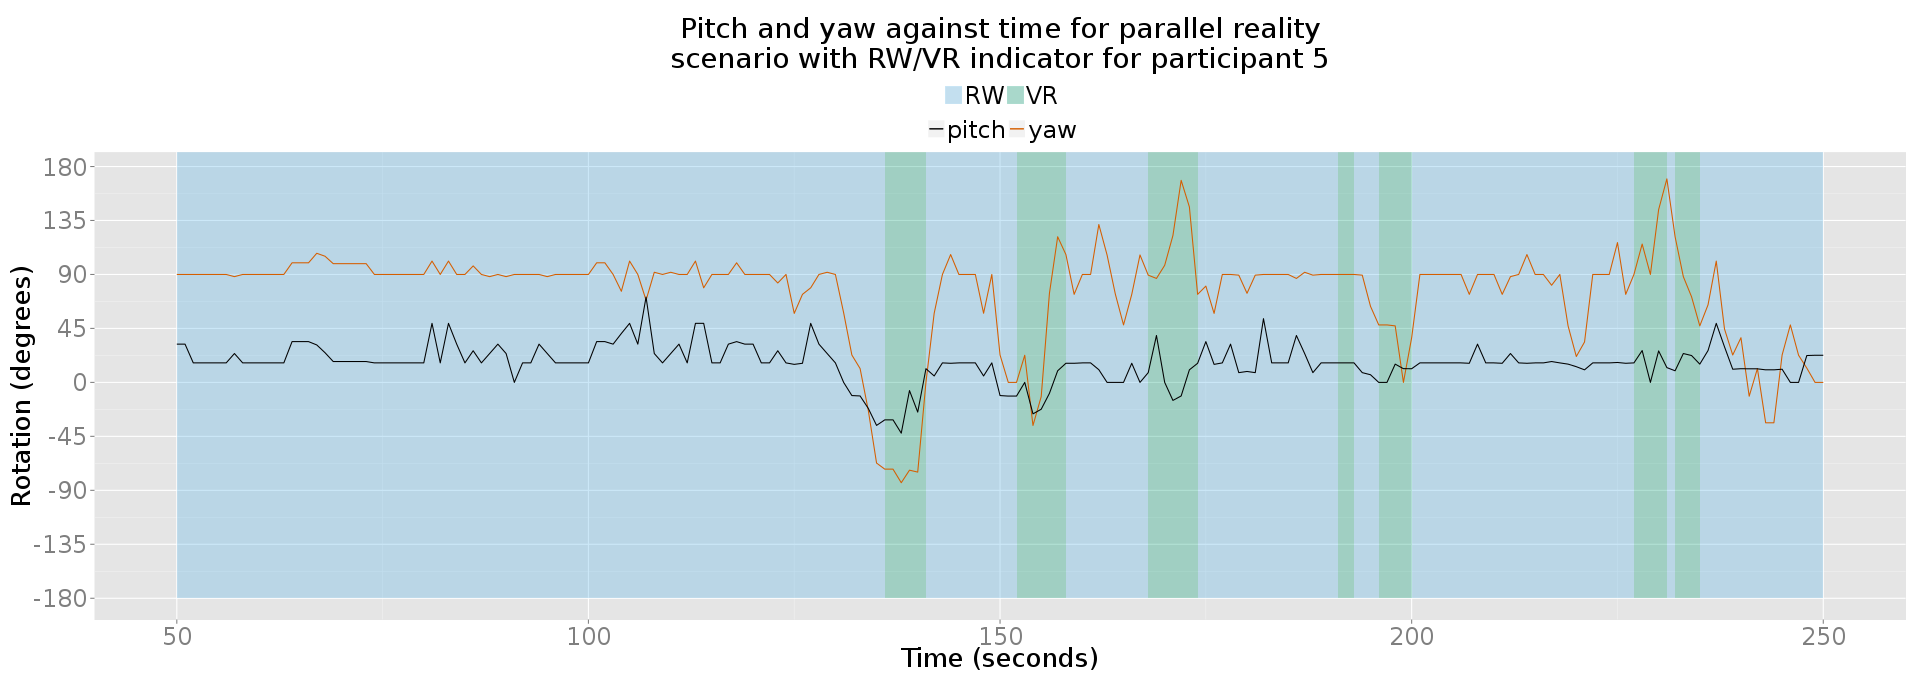
\includegraphics[width=\textwidth]{1/5_pitch_yaw.png}
	\caption{Pitch \& yaw against time for participant 5 in PR scenario, showing RW/VR periods.}
	\label{5_pitch_yaw.png}
	\end{center}
\end{figure}

Calculating the mean standard deviation in yaw for both RW \& VR periods, weighted by the duration of the periods, shows this relationship more accurately. With reference to the figures in table \ref{sdyawtab} the mean standard deviation in yaw while perceiving VR stimuli is higher than while perceiving RW stimuli for participant 1 (39.887\textdegree\ compared to 25.545\textdegree) \& even more so for participant 3 (60.636\textdegree\ compared to 11.702\textdegree). The values are closer for participant 5, due to the initial large delta in yaw just before the first transition into VR at around 130 seconds. Recalculating the weighted mean standard deviation from 150 seconds onwards to exclude this peak gives rise to the values of 36.074\textdegree\ for VR stimuli compared to 17.046\textdegree\ for RW stimuli, which is more in fitting with the impressions drawn from studying figure \ref{5_pitch_yaw.png}. The exception to this observation is participant 4, however this participant displayed very restricted head movement throughout both scenarios when compared to the other participants.

\begin{table}
\begin{center}
\begin{minipage}[t]{.47\linewidth}
\begin{center}
\begin{tabular}{|c|c|c|}
\hline

\textbf{Participant} & \textbf{RW (\textdegree)} & \textbf{VR (\textdegree)} \\

\hline

1 & 13.325 & 17.554 \\

\hline

3 & 12.194 & 24.662 \\

\hline

4 & 6.133 & 6.133 \\

\hline

5 & 12.193 & 12.797 \\

\hline

6 & 15.712 & 15.349 \\

\hline
\end{tabular}
\caption{Weighted mean sd in pitch for PR scenario.}
\label{sdpitchtab}
\end{center}
\end{minipage}
%
\begin{minipage}[t]{.47\linewidth}
\begin{center}
\begin{tabular}{|c|c|c|}
\hline

\textbf{Participant} & \textbf{RW (\textdegree)} & \textbf{VR (\textdegree)} \\

\hline

1 & 25.545 & 39.887 \\

\hline

3 & 11.702 & 60.636 \\

\hline

4 & 18.032 & 15.300 \\

\hline

5 & 23.155 & 29.274 \\

\hline

6 & 41.717 & 47.440 \\

\hline
\end{tabular}
\caption{Weighted mean sd in yaw for PR scenario.}
\label{sdyawtab}
\end{center}
\end{minipage}
\end{center}
\end{table}

Also, when considering the amount of time spent perceiving each environment in the PR scenario, several of the participants showed frequent transitioning behaviour, where they would perform many transitions \& remain perceiving the visual stimuli from each environment for only a few seconds: for participants 1, 4 \& 6, the mean times for both RW \& VR periods are all between 1.68 \& 3.4 seconds. Participant 3 spent longer perceiving each environment with a RW mean of 18.2 seconds \& a VR mean of 7 seconds. The outlier is participant 5, with a RW mean of 31.8 seconds \& a VR mean of 3.6 seconds; this was the participant who found it uncomfortable to walk while wearing the DK1, so a much longer amount of time spent perceiving RW stimuli is understandable.

\subsubsection{Comparing VR periods of PR scenario to VR section of traditional scenario}

Furthermore, comparing yaw from the VR periods of the PR scenario (table \ref{sdyawtab}) against yaw from the traditional scenario (table \ref{sdpitchyawtrad}) it can be seen that in most cases there is a noticeably less yaw change in the VR periods of the PR scenario than in the traditional scenario, leading to the conclusion that participants felt more comfortable to perform larger head movements when seated with the DK1 than when standing/walking with the DK1. Observations of participants while they performed the traditional scenario support this with several participants twisting their heads right around to look behind them without changing their direction of their virtual `movement', while when walking in the PR scenario they tended to largely look ahead \& perform larger orientation changes by instead turning their whole body to begin walking in the return direction.

Further comparing head movements between the VR section of the traditional scenario \& the VR periods of the PR scenario, the difference between the magnitude of pitch \& yaw is greater in the VR section of the traditional scenario than in the VR periods of the PR scenario. Comparing these values from tables \ref{sdpitchyawtrad}, \ref{sdpitchyawpr} \& \ref{sdpitchyawtrad} this difference exhibits as smaller variance in yaw \& roughly unchanged (only slight increased) variance in pitch for the VR periods of the PR scenario, further indicating that participants were more comfortable to look around themselves more freely in the traditional scenario than the PR scenario, leading to less overall head movement in the PR scenario than the traditional scenario.

%=========================================================================================================

\section{Stage 1 Conclusions}

In general, participant reactions to the Mirrorshades platform met the hypotheses. From the questionnaire data \& interview transcripts, participants reported that they found the PR scenario to be both more enjoyable \& more rewarding than the traditional scenario, despite the decreased usability \& comfort effected by the requirement to don \& carry a satchel of hardware \& hold devices in both hands. The PR scenario was reported as allowing easier comparison \& contrast between RW \& VR environments, leading to recognising more differences between the two environments \& a greater change in \& better understanding of the chapel than with the traditional scenario. The visual acuity afforded by the cameras \& both the accuracy \& lag of the IPS surfaced as the major detractors to the experience of the PR scenario.

From the log data, participants displayed restricted head movement throughout the PR scenario, looking to their sides \& above \& beneath themselves less when experiencing the VR chapel in the PR scenario than when experiencing the VR chapel in the traditional scenario. While this restriction does not appear to have been so great that it reduced the utility \& enjoyability of the PR scenario to beneath that of the traditional scenario, it has been observed by other researchers~\cite{Slater1998} that there is a significant positive association between reported sense of presence in a VR environment \& the amount of body movement, particularly head yaw, displayed by a participant, so reducing the negative impact that a PR system has upon a user's willingness to freely look around them will likely result in beneficial returns.

Through this first stage of evaluation the Mirrorshades platform has shown itself to be a rewarding new modality for experiencing VR content in a cultural heritage context, improving upon traditional techniques employed for the presentation of such content by allowing immediate comparison \& contrast between corresponding vantage points in both the RW \& VR environments.

%=========================================================================================================
%=========================================================================================================
%=========================================================================================================
%=========================================================================================================
%=========================================================================================================

\clearpage

\section{Stage 2 - Informing PR Implementation}

The first stage of evaluation into the Mirrorshades platform led to the conclusion that applying a mobile PR system to a cultural heritage scenario provides an experience that is more enjoyable \& engaging than a traditional virtual heritage scenario making use of immersive VR presentation via CAVE or static HMD, while also leading participants to a greater understanding of the relationships between the RW \& VR content presented to them. While certain drawbacks in the system highlighted by the first stage of evaluation, such as the visual acuity of the video see-through solution \& the lag in the IPS, could not be iterated upon due to lack of suitable technology, other aspects of the system that affect the overall PR experience could be investigated - namely the way that transitions between RW \& VR visual stimuli are performed, including whether the default view is 100\% RW or a mix of RW \& VR, as participants in stage 1 of the evaluation were furnished with only a single style of transition.

Stage 2 of the evaluation was divided into two parts. In the first (stage 2.1), evaluation focussed upon assessing participants' reactions to \& preferences toward three different transition styles, while in the second (stage 2.2), evaluation looked at reactions \& preferences in response to two different default views comprising RW/VR mixes. In terms of the combined Milgram/Waterworh model, this second stage of evaluation pertains to assessing the effect upon participants' focus of attention (\& to a lesser extent, sensus of attention) when performing oscillations along the locus axis using different techniques. Stage 2.1 investigates oscillations where the default view is 100\% RW, with participants performing oscillations between the RW extreme of the locus of attention axis \& other points upon the locus axis (such as in figure \ref{transition-rw-vr-hard.png}), while stage 2.2 looks into oscillations where the default view is a mix of RW \& VR, limiting how far toward the RW extreme of the locus axis the participant can reach (such as in figure \ref{transition-mix-vr.png}).

While stage 1 of the evaluation investigated the suitability of applying a mobile PR platform to the particular use case of virtual heritage, stage 2, while still within the same virtual heritage scenario, has wider use for informing implementation of PR systems in general \& not just within the context of virtual heritage.

%=========================================================================================================

\subsection{Evaluation Techniques}

As with the stage 1 investigation, a range of both qualitative \& quantitative data were collected. Evaluating participants' preferences toward different styles of transitioning between RW \& VR visual stimuli pertains to studying their reactions \& responses to ascertain the effect upon their focus of attention, a concept that is largely psychological in nature \& highly subjective~\cite{Ijsselsteijn2001}. Thus, subjective measures will produce the bulk of the data for evaluation, however they will again be backed up by objective log data to support or contradict any relationships that emerge.

Stage 2 participants completed the same pre-task questionnaire as the stage 1 participants \& Likert-type questionnaires that shared certain items with that from stage 1 were also used; the stage 2.1 participants completed a 12-item questionnaire (included as appendix \ref{}), while stage 2.2 participants completed a 9-item questionnaire (included as appendix \ref{}). The SUS questionnaire was not used, while post-task interviews \& loggigng were present. In addition to the Likert-type questionnaire, all stage 2 participants also completed the igroup presence questionnaire~\cite{Schubert2001} (IPQ, included as appendix \ref{appendix-igroup-presence-questionnaire}).

As presence does not have a single widely agreed upon definition \& those definitions that are commonly used, including that adopted by this thesis of \textit{the experience of being in one place or environment, even when one is physically situated in another} (see section \ref{lit-review-presencec}), are subjective in nature, attempts to quantify or `measure' the experience of presence are met with difficulty \& many different approaches have been adopted, some more or less suitable to certain scenarios than others. Broadly, these approaches can be categorised as either subjective (most commonly post task questionnaires), behavioural (measurement/observation of actions that do not stem from conscious thought) or physiological (heart rate, skin conductance, etc.)~\cite{Insko2003}.

In this categorisation system, one could consider the log data recorded by the Mirrorshades platform to provide a behavioural insight into the participants' sense of presence \& the interview \& Likert-type questionnaires to provide a subjective insight. For this second stage of evaluation where direct comparison is made between different styles of transition in hopes of ascertaining which result in less pronounced breaks in presence, the use of an established presence questionnaire was deemed a prudent addition to the evaluation techniques to inquire more directly about the sense of presence than the other evaluation techniques.

%=========================================================================================================

\subsection{Presence Questionnaires}

Due to the nature of the Mirrorshades platform most established presence questionnaires could not be directly applied,  for they are predominantly written for application to `traditional' VR scenarios in which the user is immersed in a VR (or remote, in the case of telepresence) environment at the intentional exclusion of stimuli from their RW environment. Illustrated in reference to an embodied cognition framework, the sense of presence in such a scenario is argued to develop from the construction of a spatial-functional mental model of the VR environment, through a combination of representation of bodily actions as possible in the VR environment \& suppression of incompatible sensory input from the RW environment~\cite{Schubert2001}. However considering a PR scenario within the same framework, sensory input from a RW environment that features high spatial equivalence with the VR environment is not incompatible; in fact it should be considered complimentary. Whereas a traditional VR experience attempts to create in the user's mind a new spatial-functional model that exists separate to, incompatible with \& suppressing the model of their RW surroundings, PR systems should instead be considered as enhancing the user's existing model of their RW surroundings, or alternatively as creating a complementary model that sits parallel to it.

This distinction is perhaps best explained as a difference in the use of the term `presence', which can be visualised using the combined Milgram/Waterworth model. Established presence questionnaires assess presence in terms of the user's position upon the locus of attention axis, where `a sense of presence' means a position toward the VR extreme of the axis \& `no sense of presence' means a position toward the RW extreme of the axis. In this stage of the evaluation into the Mirrorshades PR platform however, the aim of the evaluation is to assess presence in terms of the user's position upon the focus of attention axis, to assess the severity of breaks in presence defined as deflections upon the focus of attention axis from the presence extreme in the direction of the absence extreme, representing increased cognitive load caused by performing a transition between two environments. Instead of assessing allocation of locus of attention between two \textit{incompatible} sets of environmental stimuli, this stage of evaluation hoped to assess the impact that a locus of attention oscillating between \textit{complimentary} sets of environmental stimuli has upon focus of attention.

Many established presence questionnaires that feature wording \& weighting of questions associating negativity to awareness of the stimuli from the RW environment are thus unsuitable for use in assessment of a PR scenario. Whilst this approach is ideal for a traditional VR scenario in which immersion in a VR environment at the complete exclusion of the user's RW environment is the ultimate goal, it does not apply well to a PR scenario in which the ultimate goal is to imbue the user with the ability (\& desire) to transition between both RW \& VR environments, wherein maintaining an awareness of one environment while perceiving stimuli from the other is likely beneficial, rather than detrimental, to the overall experience.

For example, Witmer \& Singer's presence questionnaire~\cite{Witmer1998} poses several questions that directly enquire about aspects of the virtual environment (such as \textit{``13. How involved were you in the virtual environment experience?''}) but poses no questions that pertain to the RW environment other than a single comparison between VR \& RW (\textit{``7. How much did your experiences in the virtual environment seem consistent with your real world experiences?''}, an assessment of how well bodily actions were represented as possible in the VR environment). Other questionnaires, such as that used in an experiment by Slater \& Steed in which participants walked through a VR field of trees~\cite{Slater1998}, are less extreme in their weighting toward questions only about VR, asking questions both directly about the VR environment (\textit{``Please rate your sense of being in the field among the plants''}) but also enquiring as to the RW environment in a neutral sense (\textit{``During the time of the experience, which was strongest on the whole, your sense of being in the virtual field, or of being in the real world of the laboratory?''}). However even this still permeates an `either or' implication to the two environments, emphasising their incompatibility \& separateness.

%=========================================================================================================

\subsection{The Igroup Presence Questionnaire}

The IPQ assesses presence based upon three factors; spatial presence (SP), involvement (INV) \& realness (REAL). While SP questions assess how much bodily actions are represented as possible in the VR environment \& REAL questions assess the `realness' of the VR environment by eliciting direct comparisons with the RW environment, INV questions assess suppression of incompatible sensory input from the RW environment but are not worded in a manner that presents attention paid to this sensory input as negative (or even such that these stimuli are considered incompatible), reducing risk of negative bias when the questionnaire is applied to a scenario in which attention paid to RW stimuli is encouraged.

For a well implemented traditional VR experience that elicits a high sense of (virtual) presence in the user, one would expect their IPQ results to score highly in all three factors. As discussed by Constantin~\cite{Constantin2003a}, SP3 (\textit{``I did not feel present in the virtual space''}, anchored between \textit{``did not feel''} \& \textit{``felt present''}) \& INV2 (\textit{``I was not aware of my real environment''}, anchored between \textit{``fully disagree''} \& \textit{``fully agree''}) would seem to be fairly directly tied together, as a high involvement in the RW environment would intuitively reduce spatial presence by hampering the sense that bodily actions are possible in the VR environment.

However, in a PR scenario that features high spatial equivalence between its constituent RW \& VR environments, this tie between SP \& INV may not demonstrate. Due to the spatial equivalence between the two environments, bodily actions in the VR environment are inherently compatible with those in the RW environment, so SP may score highly even when INV scores low, as RW sensory input isn't suppressed but in fact encouraged. In fact, it may even be the case that an inverse relationship presents between SP3 \& INV2, as heightened awareness of the RW environment leads the user to a more believable representation of bodily actions in the VR enviroonment as possible, increasing SP as (inherently possible) RW bodily actions are shared (`possible') with the VR environment. A restrained expectation would be for a PR scenario to present in general lower INV scores than the traditional scenario but without drastically reducing SP scores, whilst a more optimistic expectation would be for lower INV scores \& \textit{heightened} SP scores - that reinforcement of bodily actions within the RW environment will lead to an increase in experienced spatial presence in the VR environment.

%=========================================================================================================

%there isn't really a mapping from SP/INV/REAL to focus/locus/sensus.
% INV kinda maps to locus & effects focus

% ***but why didn't we add physiological measures as well?

%=========================================================================================================

\subsection{Design of Scenarios}

Both stages 2.1 \& 2.2 followed a similar pattern to the stage 1 evaluation. Participants first received a `traditional' VR experience by using the DK1 \& Xbox controller to explore the VR chapel while seated \& subsequently completed the IPQ in order to produce baseline IPQ results for a traditional experience of the chapel model viewed via the DK1. In stage 2.1 the participants then performed two PR scenarios in which they walked through the RW/VR chapels. In the first scenario the default view on the DK1 screen was 100\% RW \& they were granted access to 3x different transition styles;

\begin{enumerate}
	\item hard switch (see section \ref{sub-hardswitch}) mapped to controller \texttt{[A]} button (transition 1)
	\item transition with linear interpolation (see section \ref{transition-with-linear-interpolation}) mapped to controller \texttt{[B]} button (transition 2)
	\item analogue selectable opacity (see section \ref{analogue-selectable-opacity}) mapped to controller right trigger \texttt{[RT]} (transition 3)
\end{enumerate}

In the first stage 2.1 scenario pressing \& holding the \texttt{[A]} button triggered a hard switch from 100\% RW to 100\% VR, pressing \& holding the \texttt{[B]} button triggered a linear interpolated switch from 100\% RW to 100\% VR \& pulling on the right trigger \texttt{[RT]} reduced the opacity of the game objects upon which the camera feeds were rendered from 100\% to an amount that mapped to the amount that the trigger was pulled (pulling the trigger all the way in would reduce the opacity of the objects to 0\% \& thus display 100\% VR, pulling the trigger 33\% would reduce the opacity of the objects by 33\% \& thus display 66\% RW \& 33\% VR, etc.). In the second stage 2.1 scenario they were granted access to the same 3x transitions via the Xbox controller \& additionally a 4th transition of the periodic hard switch (see section \ref{subsub-periodic}) was triggered every 3 seconds for a duration of 0.15 seconds. These two scenarios are referred to as `scenario 1-3' \& `scenario 1-4', respectively.

In stage 2.2, participants again performed two PR scenarios in which they walked through the RW/VR chapels, this time with only a single transition style available (the transition with linear interpolation) but with the default view set at 75\% RW/25\% VR in the first \& at 50\% RW/50\% VR in the second.

Rather than describing a path through the chapel with particular positions of interest to stop \& look around at, participants were simply told to slowly make their way from the starting position down to the altar end of the chapel. For at least one participant in the stage 1 evaluation, their exploration of the environments seemed to be subdued by their adherence to the prescribed route. In order to promote a more natural style of exploration the route description was not used in the second stage of evaluation.

%=========================================================================================================

\subsection{Hypotheses}

It was hypothesized that

correlation between which type of transition participants favoured \& the situation they were in (walking, standing still, etc.)



It is hypothesized that a manner of transitioning between visual stimuli which results in a less severe BIP will be preferable to a manner of transitioning which results in a worse BIP. As focus in the Waterworth model is most closely related to presence in the VR literature~\cite{Waterworth2001}, one of the subjective measures that will be used in this evaluation will be an established presence measure, to try to capture the behaviour of the user's position upon the focus axis.


These data are expected to reveal relationships between various different metrics \& the choice of transition methods. For example, it is expected that participants will perform short transitions to VR or transitions to a mix of RW \& VR when moving \& perform longer transitions to VR when stationary. This kind of relationship will support or contradict the subjective data collected through questionnaire \& interview.

%=========================================================================================================

\section{Stage 2.1 Results}

A total of 7 participants completed the stage 2.1 evaluation;
\begin{itemize}
	\item Age range from 18 to 27, with a mean of 22.3 \& a standard deviation of 4
	\item 5x identified as male \& 2x as female
	\item All reported previous experience with a games console controller
	\item None reported previous experience with a HMD
	\item 2x reported having previously visited the chapel
	\item None reported having previously experienced the virtual chapel
\end{itemize}

%=========================================================================================================

\begin{figure}[h]
	\begin{center}
	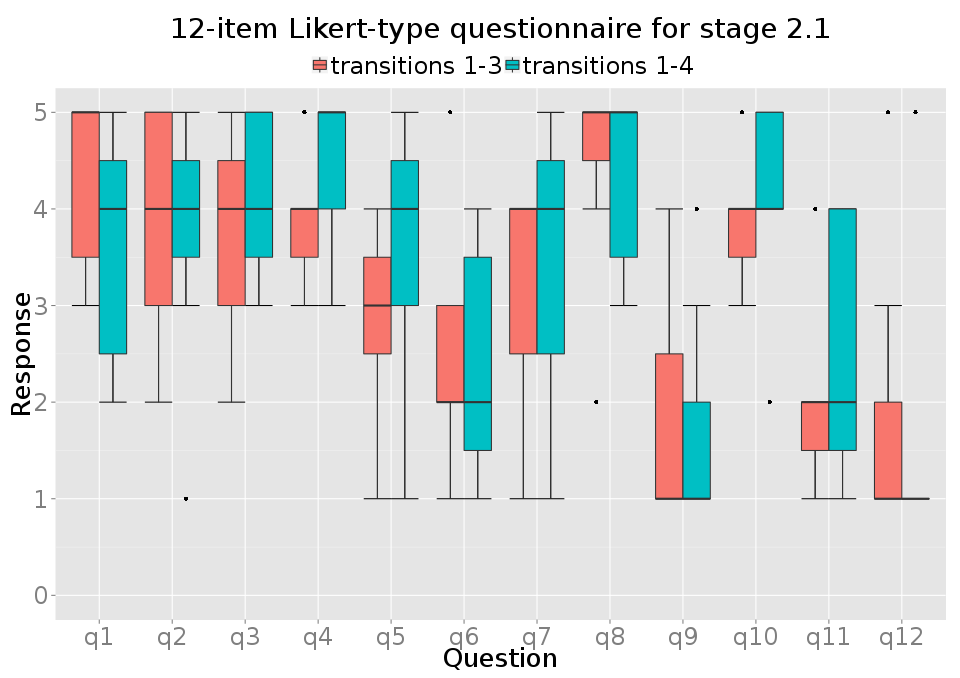
\includegraphics[width=.6\textwidth]{2.1/12-item-likert-type-questionnaire-boxplot.png}
	\caption{Likert-type questionnaire results for stage 2.1.}
	\label{2-1-12-item-likert-type-questionnaire-boxplot.png}
	\end{center}
\end{figure}

%=========================================================================================================

\subsection{Likert-type Questionnaires}

When considering the responses to the Likert-type questionnaires (see figure \ref{2-1-12-item-likert-type-questionnaire-boxplot.png}) for the two PR scenarios of the stage 2.1 evaluation, the following observations can be made.

\begin{itemize}
	\item Participants found the scenario 1-3 more enjoyable than scenario 1-4 (q1)
	\item Preference toward one transition style over others was more varied \& in general less in scenario 1-3 than in scenario 1-4 (q2)
	\item Participants were more aware of both environments in scenario 1-4 than in scenario 1-3 (q3)
	\item Participants found it easier to compare features from past \& present in scenario 1-4 than in scenario 1-3 (q4)
	\item Participants preferred to use one transition more than others in certain situations more in scenario 1-4 than they did in scenario 1-3 (q5)
	\item Slightly more motion sickness was reported in scenario 1-4 (q7)
	\item Participants found scenario 1-3 to be a more rewarding way to explore the chapel (q8)
	\item Participants found that scenario 1-4 gave them a better understanding of what the chapel was like in the past (q10)
	\item Participants found switching between RW \& VR more uncomfortable in scenario 1-4 than in scenario 1-3 (q11)
	\item Participants reported not noticing differences slightly more in scenario 1-3 than in scenario 1-4
\end{itemize}

%=========================================================================================================

\subsection{Interview Transcripts}

Once again, recordings of the structured interviews were transcribed after the chapel sessions \& provided a wealth of qualitative insight into the participants' experiences with the Mirrorshades platform during the stage 2.1 evaluation.

Every single participant said that they preferred scenario 1-3 over scenario 1-4. In particular, one participant  reported that each time scenario 1-4 triggered an automatic transition (transition 4), s/he had to stop to regain their bearings, with another reporting that each transition 4 meant having to having to \textit{``stop \& work it out again''}. Several participants noted that they felt more `in control' during scenario 1-3 than during scenario 1-4. Transition 4 was reported as being particularly off-putting when inaccuracy in the IPS had placed the virtual vantage at a position notably different to the participant's real position, especially when this resulted in virtual \& real positions being on opposite sides of a wall.

Roughly half of the participants said that scenario 1-3 was more engaging, another found the scenarios roughly similar with regards to engagement \& 2x found scenario 1-4 to be more engaging although they mentioned that they suspected this could simply have been down to increased familiarity with the system. Several participants said that transition 4 was `unexpected', leading to a less `consistent' experience.

Responses were mixed when asked about whether one scenario allowed them to perceive more differences between RW \& VR in one scenario compared to the other. 3x reported experiencing no difference between the scenarios in this regard. 2x answered that they found scenario 1-3 better, one because the flash threw him/her off, the other because \textit{``you could fade between''}  although this feature (transition 3) was available in both scenarios. 2x chose 1-4 as better, one because transition 4 would happen when s/he wasn't prepared for a transition \& thus s/he would \textit{``notice that something had moved, whereas if I knew I was switching I would maybe subconsciously expecting things to move''}.

All but one participant reported preferring transition 3 accessed via the right trigger \texttt{[RT]} to the other transitions. The one participant who answered otherwise elaborated that they did not notice much difference between the different transition styles \& when thinking back to the scenarios was \textit{``not sure which one I was using now!''}. Looking at the log data for this participant however (see section \ref{2-1-log-data}) this participant did nonetheless make use of all the transition styles in both scenarios 1-3 \& 1-4, heavily favouring the hard switch transition 1 in scenario 1-4.

When asked why they preferred transition 3, participants reported liking how being able to control the opacity allowed them to \textit{``see elements of both''} environments at once, to \textit{``simultaneosuly measure the historical differences''}, with the trigger giving them more `control'.

Responses when asked about motion sickness varied greatly. One participant reported none at all in either scenario, while one reported some motion sickness when seated \& using the analogue stick of the Xbox controller to turn their virtual presence \& also when walking in the PR scenario when the IPS was inaccurate. One participant reported motion sickness that increased with time, being comfortable for the first 2/3rds of each scenario \& with both PR scenarios being worse than the traditional seated scenario. Three participants reported motion sickness only when walking in the PR scenarios; of these, one reported that it was worse in scenario 1-4 \& another said that motion sickness only occurred when looking at RW via the cameras. One participant only experienced motion sickness after removing the DK1.

Other comments included not knowing where they were in the chapel inducing motion sickness \& that accuracy of the IPS needed improvement, with sudden large VR movements inducing motion sickness. Furthermore, one participant commented directly upon the relationship between `immersion' \& perceived realism of the VR environment - \textit{``\ldots obviously it wasn't the same quality, but I still felt so immersed in it. Even though part of me would've known it wasn't real, most of it felt real even though it didn't look like it''}.

%=========================================================================================================

\subsection{Log Data}
\label{2-1-log-data}

Log data were recorded during all scenarios, however these data were not recorded for 4 out of the 7 participants for the traditional seated scenario thus detailed comparisons cannot reasonably be made between the traditional scenario \& the PR scenarios. Log data were however successfully recorded for both PR scenarios \& as such comparisons can be made between the PR scenarios \& within each PR scenarios.

%=====================

\subsubsection{Comparing traditional \& PR scenarios}

For all participants there was again substantially more yaw change than pitch change, in both traditional \& PR scenarios. Figure \ref{2-1-8-pitch-yaw-trad-1-3-1-4.png} shows this relationship by plotting pitch \& yaw against time for participant 8 for all three scenarios (traditional at left, scenario 1-3 in the middle \& scenario 1-4 at right) \& the standard deviations for all participants across all three scenarios is given by tables \ref{2-1-sd-trad}, \ref{2-1-sd-1-3} \& \ref{2-1-sd-1-4}.

\begin{figure}[h]
	\begin{center}
	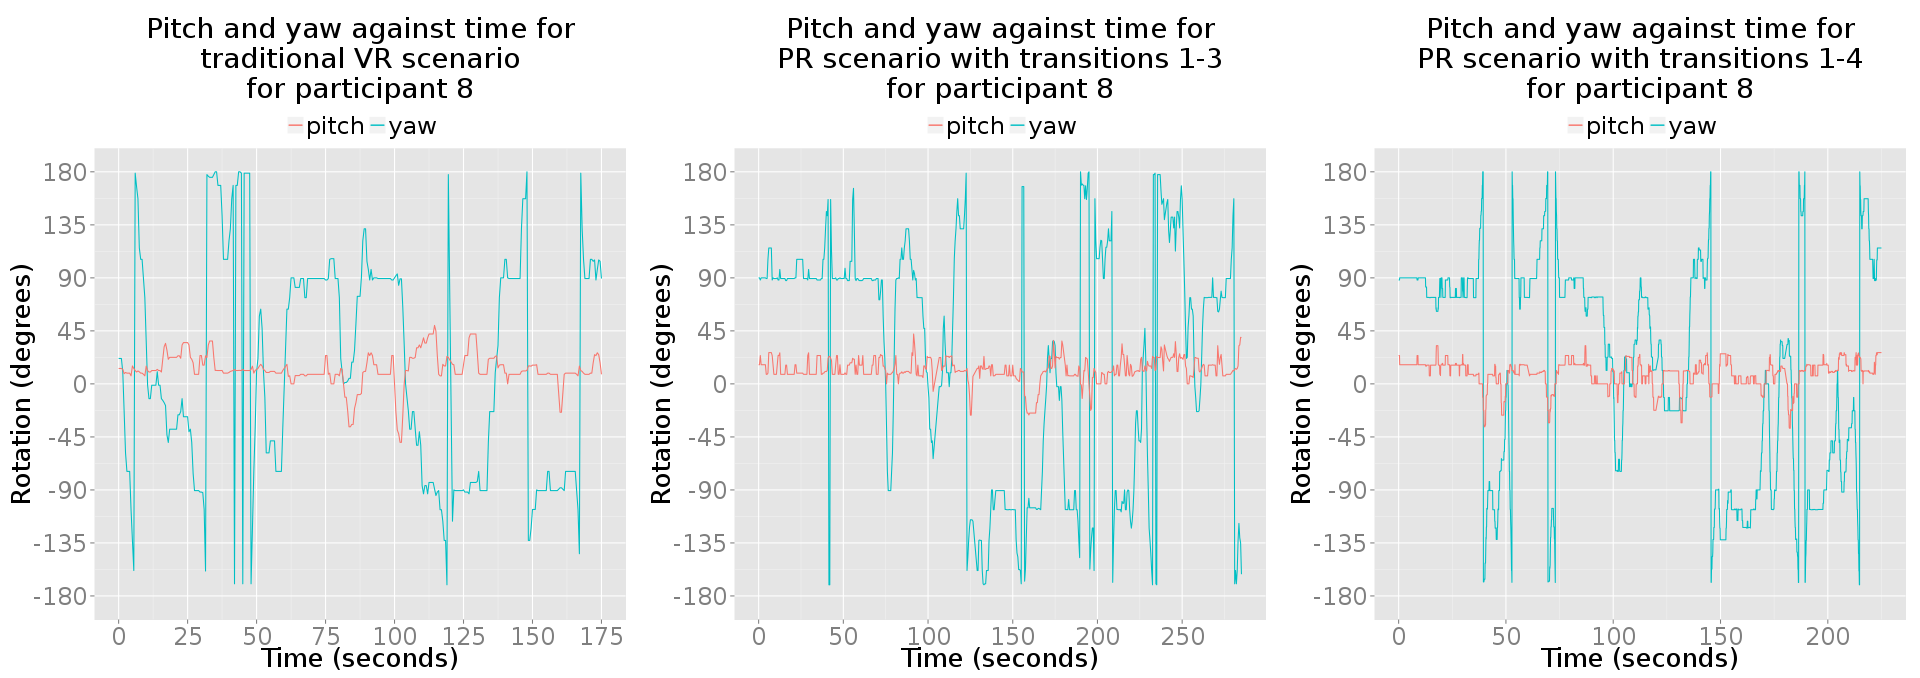
\includegraphics[width=\textwidth]{2.1/8-pitch-yaw-trad-1-3-1-4.png}
	\caption{Pitch \& yaw against time for participant 8 in traditional \& both PR scenarios.}
	\label{2-1-8-pitch-yaw-trad-1-3-1-4.png}
	\end{center}
\end{figure}

\begin{table}
\begin{center}
\begin{minipage}[t]{.47\linewidth}
\begin{center}
\begin{tabular}{|c|c|c|}
\hline

\textbf{Participant} & \textbf{Pitch (\textdegree)} & \textbf{Yaw (\textdegree)} \\

\hline

7 & 13.013 & 87.822 \\

\hline

8 & 13.917 & 94.436 \\

\hline

9 & 12.039 & 87.956 \\

\hline

10 & no data & no data \\

\hline

11 & no data & no data \\

\hline

12 & no data & no data \\

\hline

13 & no data & no data \\

\hline

\end{tabular}
\caption{Standard deviation in pitch \& yaw for traditional scenario.}
\label{2-1-sd-trad}
\end{center}
\end{minipage}
\end{center}
\end{table}

\begin{table}
\begin{center}
\begin{minipage}[t]{.47\linewidth}
\begin{center}
\begin{tabular}{|c|c|c|}
\hline

\textbf{Participant} & \textbf{Pitch (\textdegree)} & \textbf{Yaw (\textdegree)} \\

\hline

7 & no data & no data \\

\hline

8 & 10.253 & 102.254 \\

\hline

9 & 13.734 & 84.076 \\

\hline

10 & 17.833 & 84.578 \\

\hline

11 & 11.540 & 76.445 \\

\hline

12 & 19.635 & 74.696 \\

\hline

13 & 22.095 & 91.827 \\

\hline
\end{tabular}
\caption{Standard deviation in pitch \& yaw for PR scenario with transitions 1-3 (RW \& VR periods combined).}
\label{2-1-sd-1-3}
\end{center}
\end{minipage}
%
\begin{minipage}[t]{.47\linewidth}
\begin{center}
\begin{tabular}{|c|c|c|}
\hline

\textbf{Participant} & \textbf{Pitch (\textdegree)} & \textbf{Yaw (\textdegree)} \\

\hline

7 & no data & no data \\

\hline

8 & 11.493 & 89.531 \\

\hline

9 & 12.365 & 95.144 \\

\hline

10 & 14.059 & 90.429 \\

\hline

11 & 8.354 & 82.279 \\

\hline

12 & 22.202 & 75.425 \\

\hline

13 & 19.530 & 62.321 \\

\hline
\end{tabular}
\caption{Standard deviation in pitch \& yaw for PR scenario with transitions 1-4 (RW \& VR periods combined).}
\label{2-1-sd-1-4}
\end{center}
\end{minipage}
\end{center}
\end{table}

\textbf{Can't really compare between traditional \& PR, however for what we do have of traditional they exhibit this more yaw than pitch relationship. This is the same as for stage 1.}

%=====================

\subsubsection{Comparing RW \& VR periods within PR scenarios}

When comparing pitch \& yaw data between the RW \& VR periods within the two PR scenarios, five out of the seven participants displayed greater change in yaw when perceiving VR stimuli than when perceiving RW stimuli for both scenario 1-3 \& scenario 1-4. Figure \ref{8-1-3-pitch-yaw.png} illustrates this relationship for participant 8 undertaking scenario 1-3 while figure \ref{12-1-4-pitch-yaw.png} illustrates the relationship for participant 12 undertaking scenario 1-4.

\begin{figure}[h]
	\begin{center}
	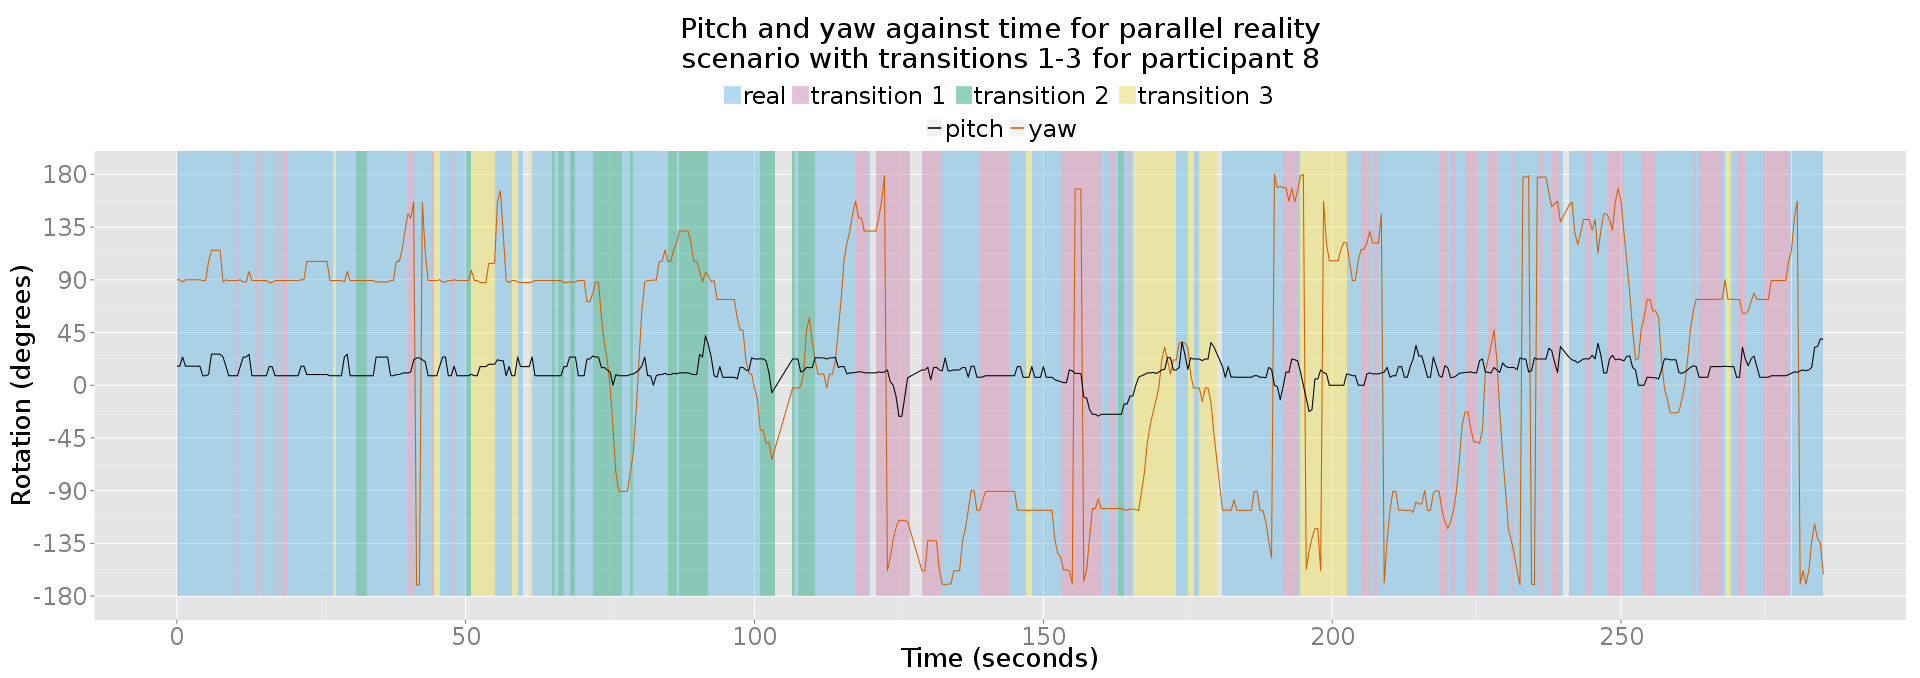
\includegraphics[width=\textwidth]{2.1/8-1-3-pitch-yaw.png}
	\caption{Pitch \& yaw against time for participant 8 in scenario 1-3, showing RW/VR transitions.}
	\label{8-1-3-pitch-yaw.png}
	\end{center}
\end{figure}

%\begin{figure}[h]
%	\begin{center}
%	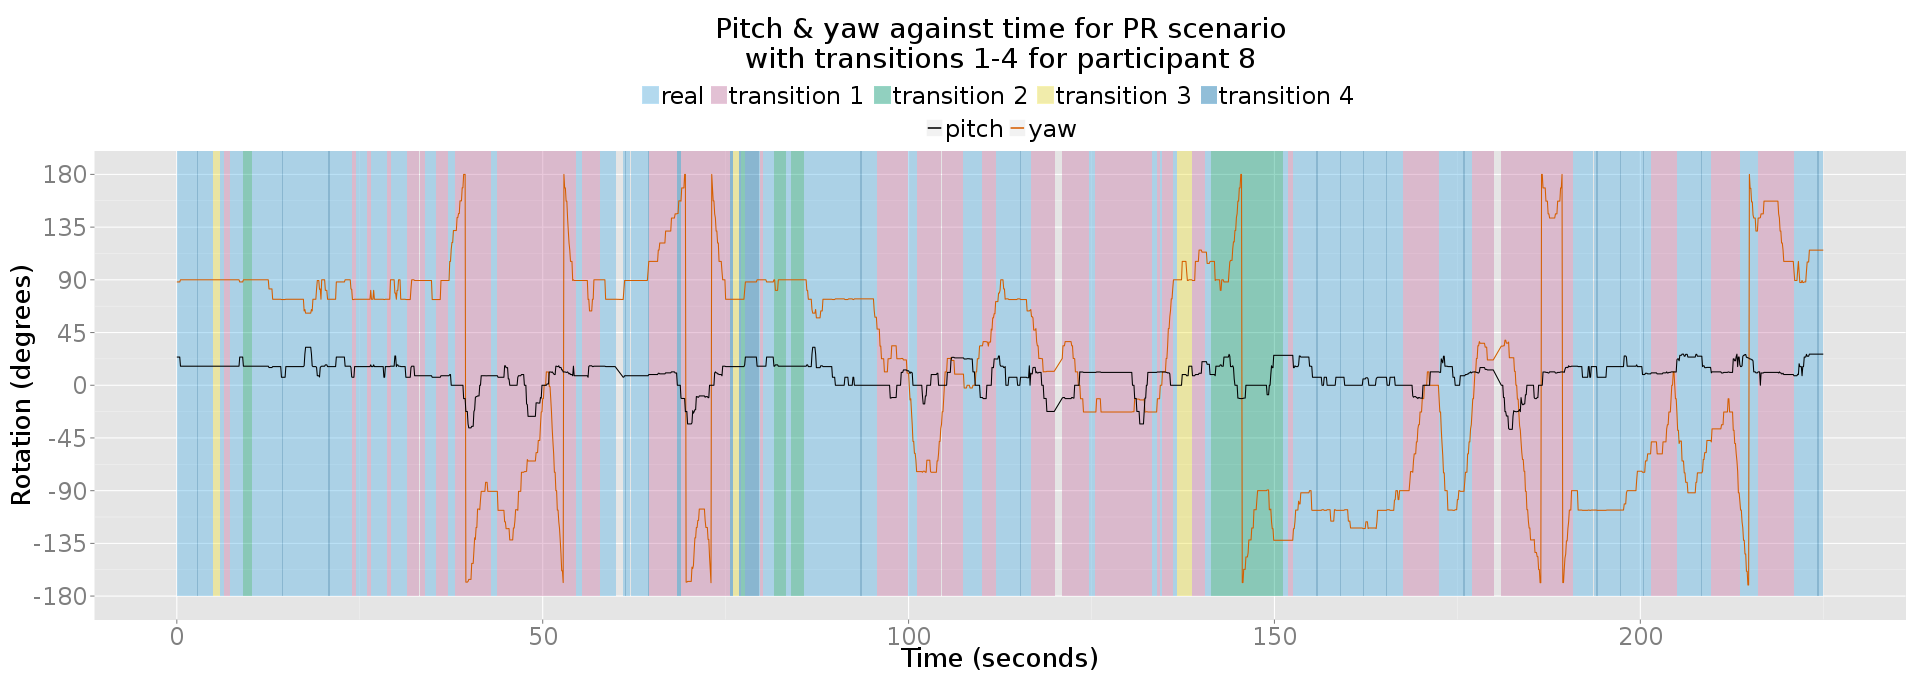
\includegraphics[width=\textwidth]{2.1/8-1-4-pitch-yaw.png}
%	\caption{Pitch \& yaw against time for participant 8 in scenario 1-4, showing RW/VR transitions.}
%	\label{8-1-4-pitch-yaw.png}
%	\end{center}
%\end{figure}

\begin{figure}[h]
	\begin{center}
	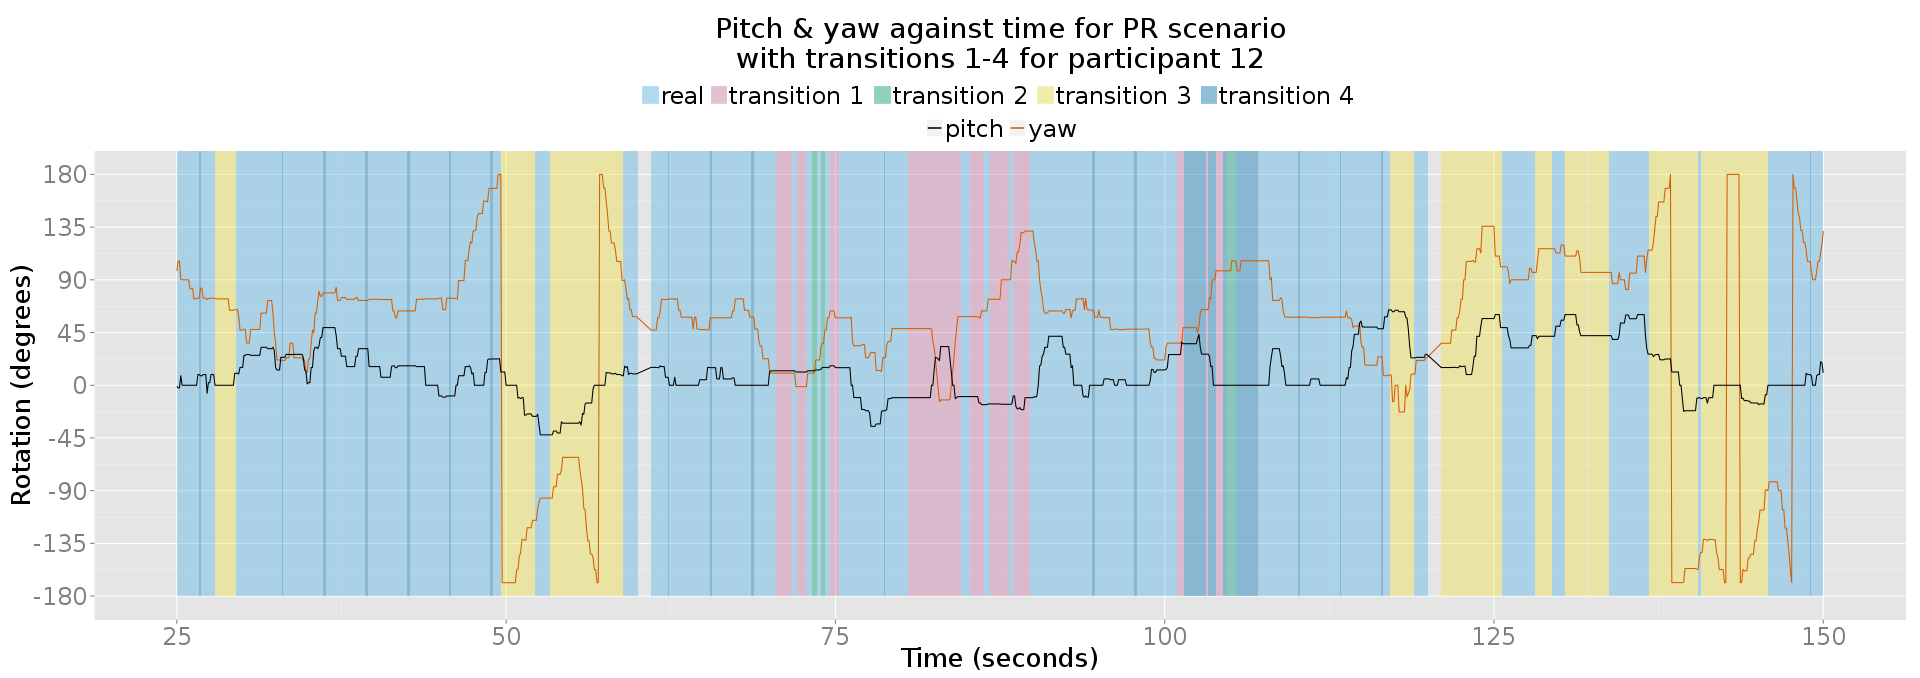
\includegraphics[width=\textwidth]{2.1/12-1-4-pitch-yaw.png}
	\caption{Pitch \& yaw against time for participant 12 in scenario 1-4, showing RW/VR transitions.}
	\label{12-1-4-pitch-yaw.png}
	\end{center}
\end{figure}

\textbf{Difference between yaw change in real \& virtual greater in 1-4 than in 1-3, though this could be familiarity.}

When comparing head movement, as mean standard deviation weighted by duration of the periods, between the RW \& VR portions of the PR scenarios, for most participants there is larger change in yaw during VR periods than RW periods of scenario 1-3 (see table \ref{mean-sd-yaw-1-3}), however the difference is not great. When considering the same criteria for scenario 1-4 (see table \ref{mean-sd-yaw-1-4}) however, all participants display greater change in yaw during VR periods, most quite substantially so. At the same time, all participants in scenario 1-4 showed less change in yaw in the RW periods than in the RW periods of scenrio 1-3. Whilst this apparent increased comfort with larger head movements in VR could be explained due to familiarity, the magnitude of the difference between scenario 1-3 \& scenario 1-4 makes it hard to believe that familiarity is the sole reason. \textbf{And because scenario 1-4 is not really that different to 1-3 (it's just the addition of the automatic switch).}

\begin{table}
\begin{center}
\begin{minipage}[t]{.47\linewidth}
\begin{center}
\begin{tabular}{|c|c|c|}
\hline

\textbf{Participant} & \textbf{RW (\textdegree)} & \textbf{VR (\textdegree)} \\

\hline

7 & no data & no data \\

\hline

8 & 41.680 & 42.228 \\

\hline

9 & 19.274 & 31.133 \\

\hline

10 & 13.541 & 16.758 \\

\hline

11 & 28.030 & 16.751 \\

\hline

12 & 38.654 & 28.494 \\

\hline

13 & 29.623 & 39.717 \\

\hline
\end{tabular}
\caption{Weighted mean sd in yaw for scenario 1-3.}
\label{mean-sd-yaw-1-3}
\end{center}
\end{minipage}
%
\begin{minipage}[t]{.47\linewidth}
\begin{center}
\begin{tabular}{|c|c|c|}
\hline

\textbf{Participant} & \textbf{RW (\textdegree)} & \textbf{VR (\textdegree)} \\

\hline

7 & 20.228 & 50.963 \\

\hline

8 & 10.783 & 50.593 \\

\hline

9 & 13.579 & 27.398 \\

\hline

10 & 10.7334 & 34.981 \\

\hline

11 & 13.500 & 13.513 \\

\hline

12 & 16.248 & 50.326 \\

\hline

13 & 7.269 & 57.162 \\

\hline
\end{tabular}
\caption{Weighted mean sd in yaw for scenario 1-4.}
\label{mean-sd-yaw-1-4}
\end{center}
\end{minipage}
\end{center}
\end{table}

%=====================

\subsubsection{Other}

Looking at individual participants in more detail leads to some interesting observations.

`Trying out' transitions
	participant 7 scenario 1-4 shows
	participant 9 scenario 1-3 \& 1-4
	participant 11 scenario 1-3 \& 1-4
	participant 13 1-3 \& 1-4

Movement vs head movement
	participant 8 all(?)
	participant 9 traditional, 1-3 \& 1-4
	participant 13 1-3

Time spent in virtual
	participant 8 - more time spent in VR in 1-4 to avoid the automatic switch
	participant 9 - more time spent in VR because of better understanding what they were meant to be doing (familiarity)
	
Other
	participant 12 - all big head movements in 1-4 were in VR, but in 1-3 there was RW head movement too?








Number of transitions in each session ranged from high teens to low sixties.

Mean times spent in real/virtual are much closer than in stage 1.

four of seven participants spent more time in real than virtual in both 1-3 \& 1-4
	for three participants the ratio was closer in 1-4 than in 1-3
	one spent more time in virtual than real in both 1-3 \& 1-4
	one spent more time in real in 1-3 \& then more time in virtual tin 1-4 (familiarity?)
	
`Trying out', clearly visible in participant

***plots showing opacity of some participants actually using the trigger not all the way down


%=========================================================================================================

\subsection{IPQ}


%=========================================================================================================













%=========================================================================================================

\clearpage

\subsubsection{Participant 7}

\begin{figure}[h]
	\begin{center}
	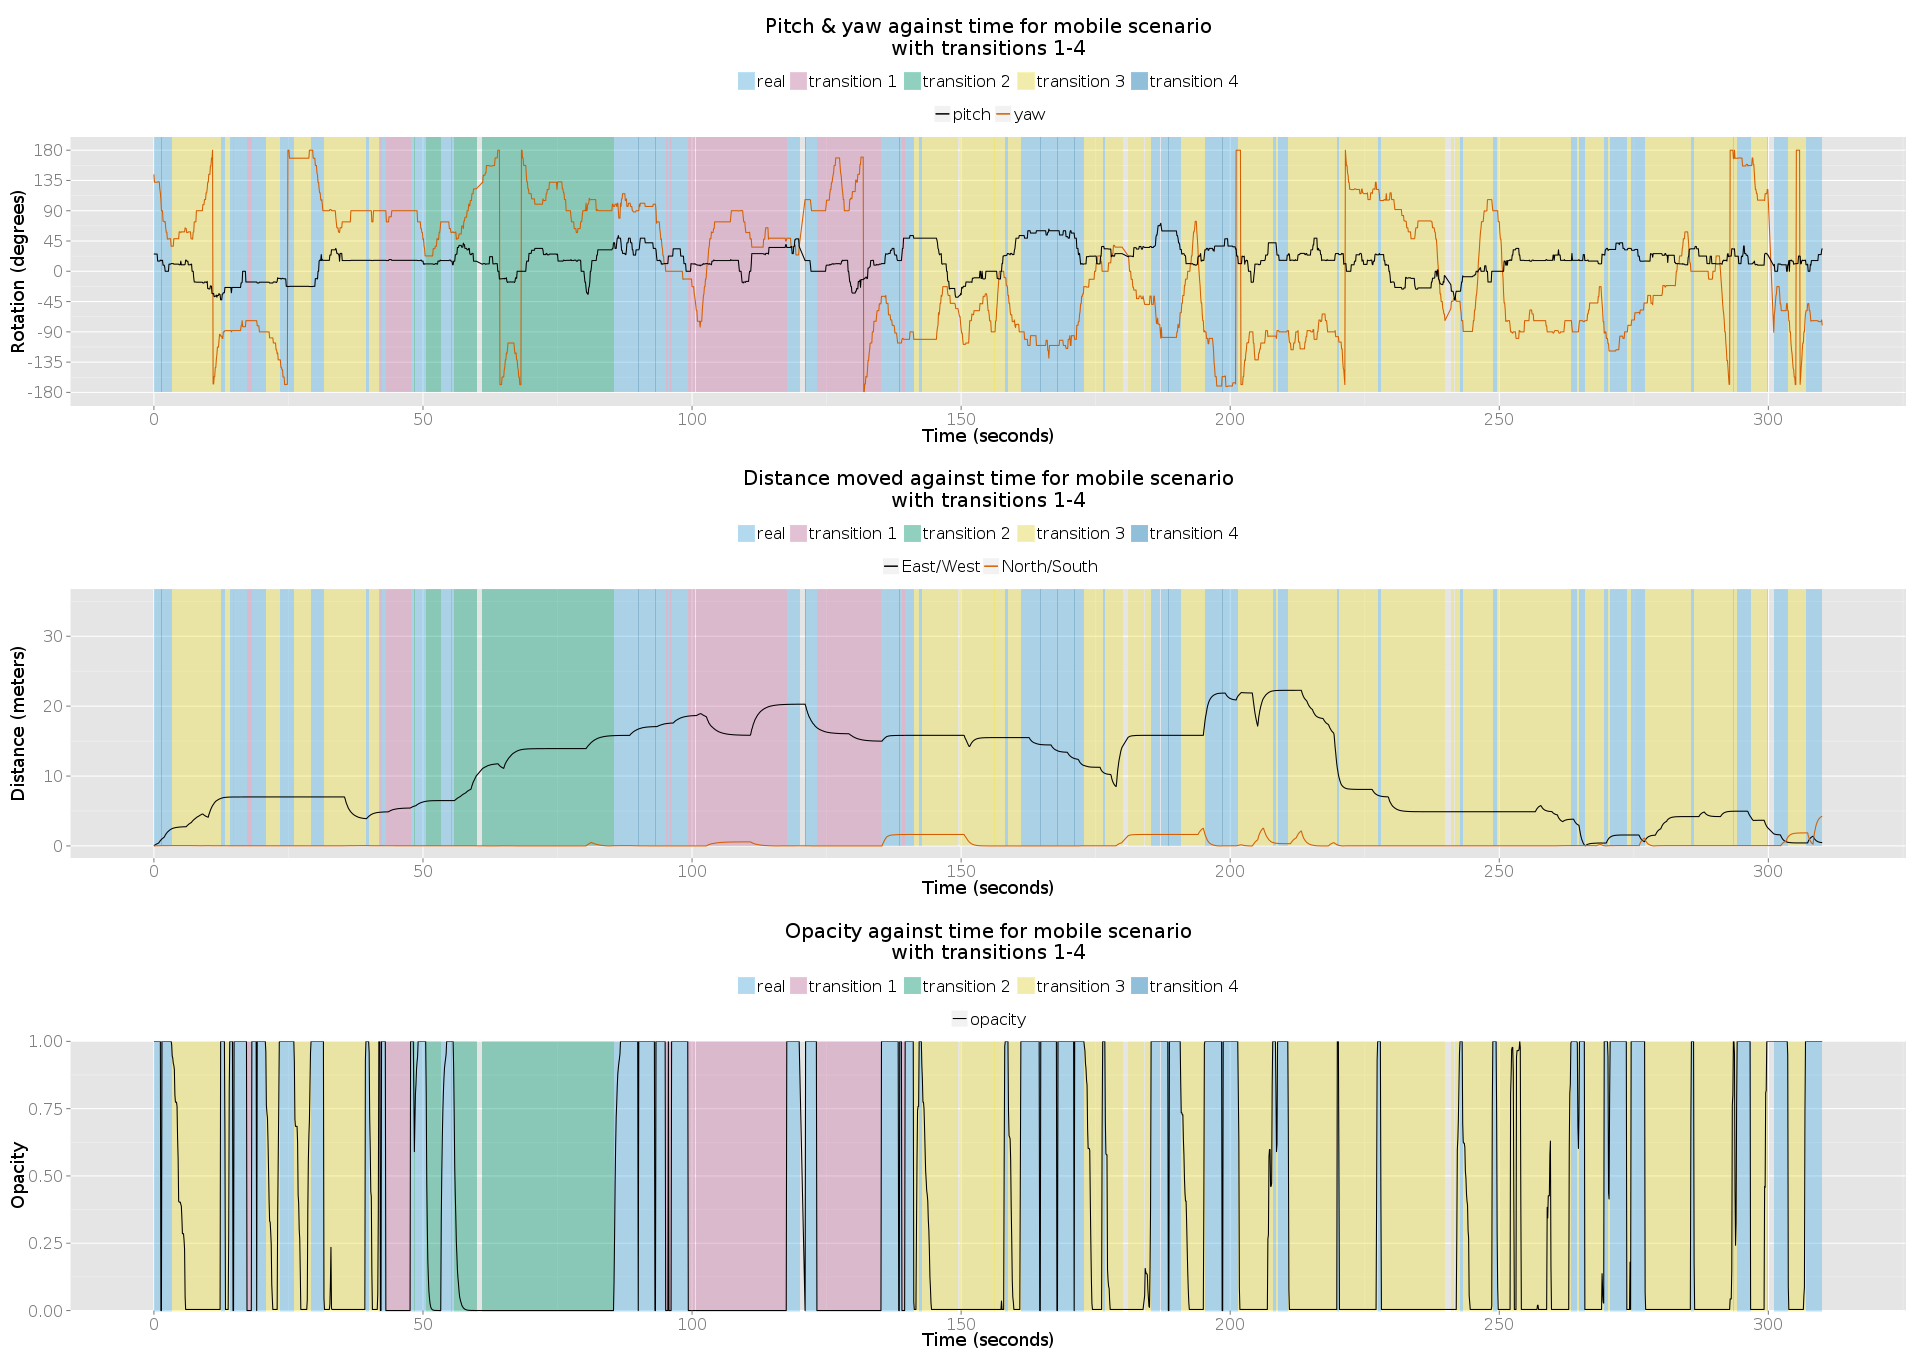
\includegraphics[width=\textwidth]{2.1/7_1-4_3up.png}
	\caption{Some images, yah.}
	\end{center}
\end{figure}

%=========================================================================================================

\clearpage

\subsubsection{Participant 8}

\begin{figure}[h]
	\begin{center}
	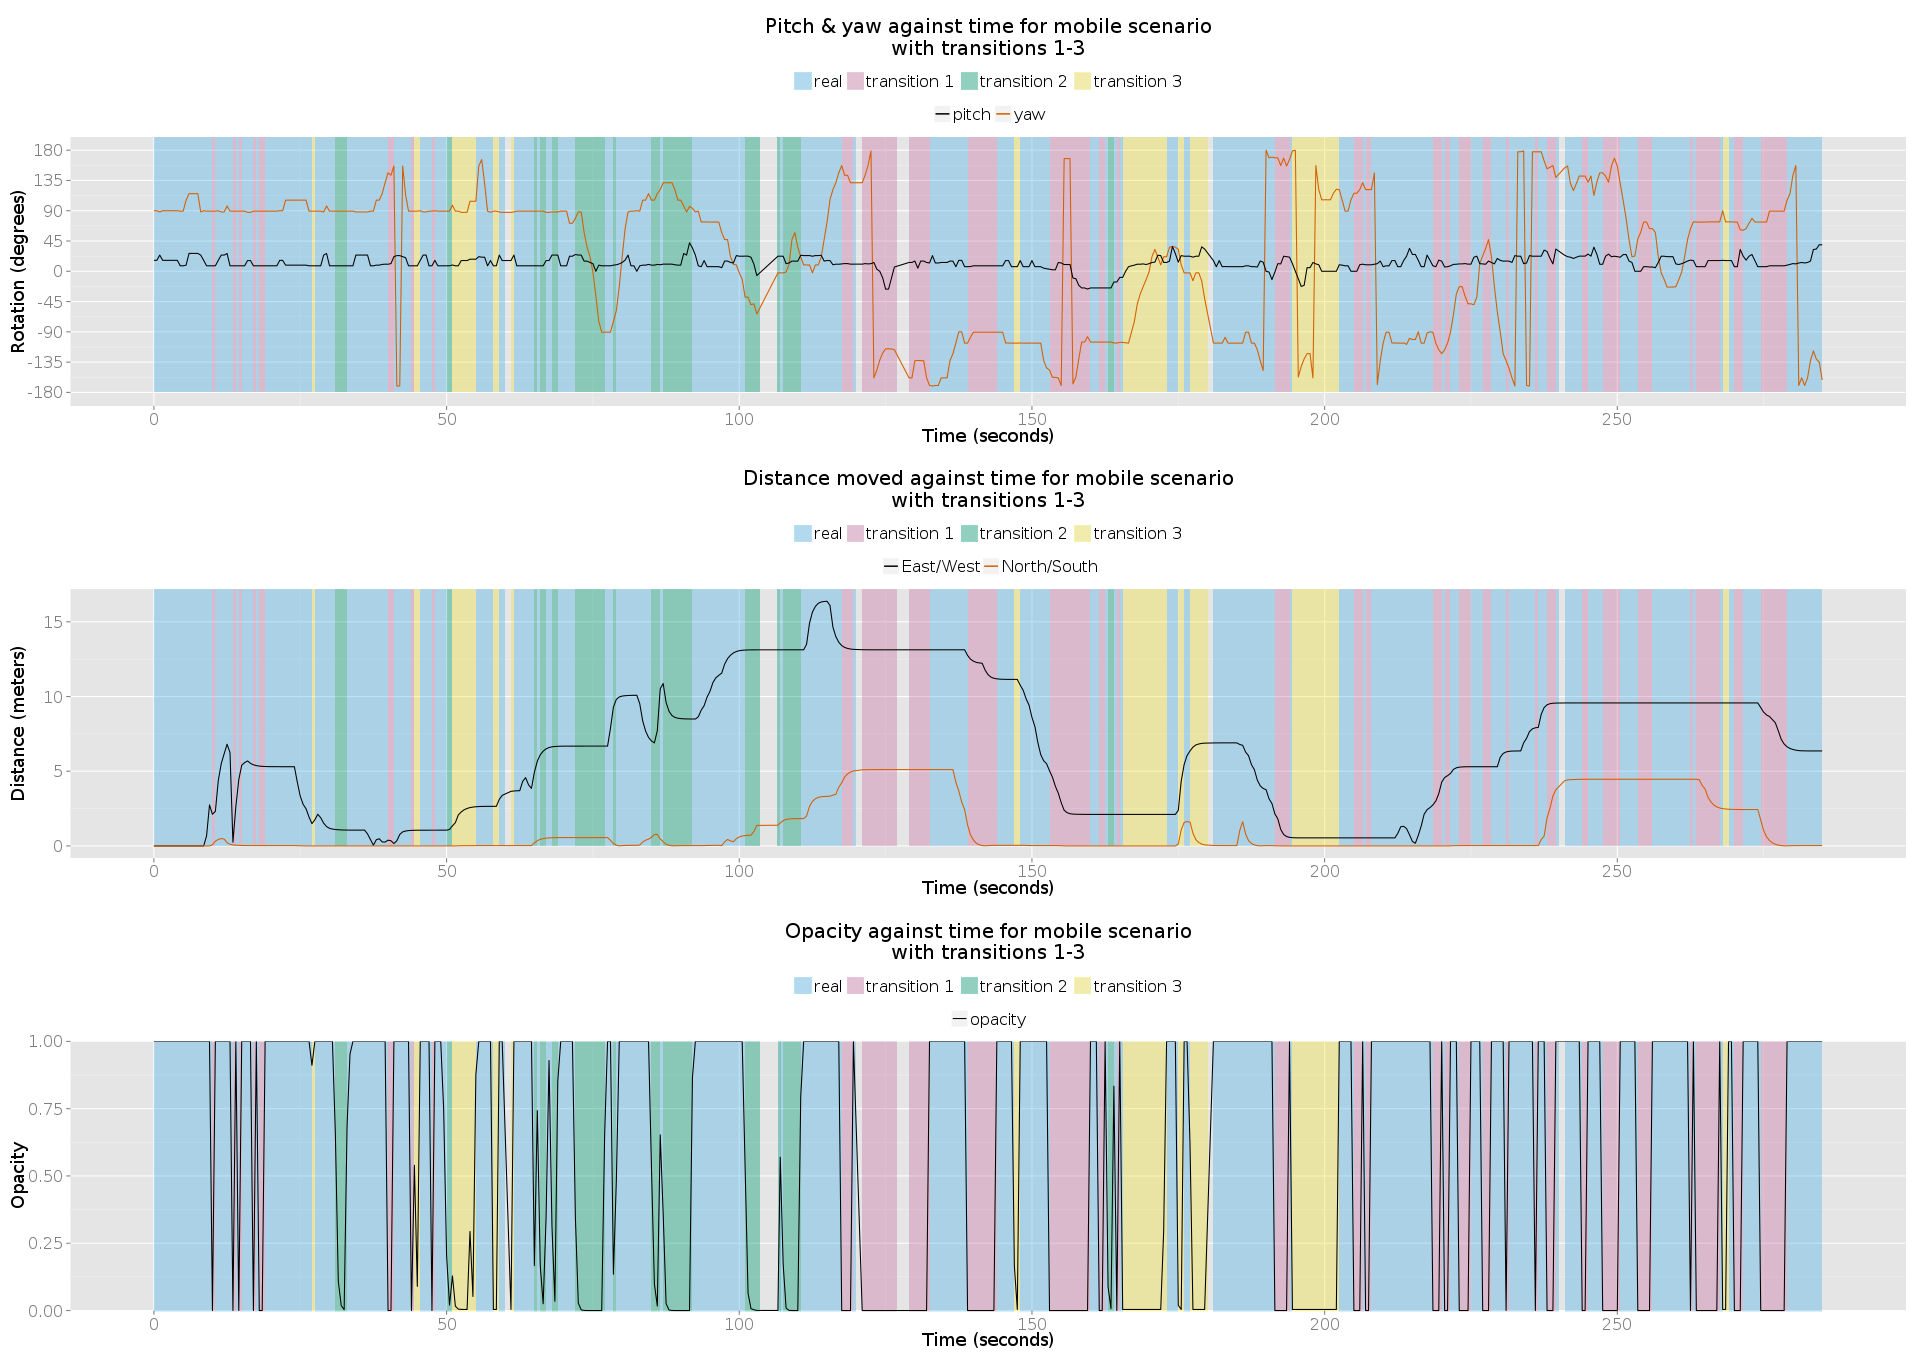
\includegraphics[width=\textwidth]{2.1/8_1-3_3up.png}
	\caption{Some images, yah.}
	\end{center}
\end{figure}

\clearpage

\begin{figure}[h]
	\begin{center}
	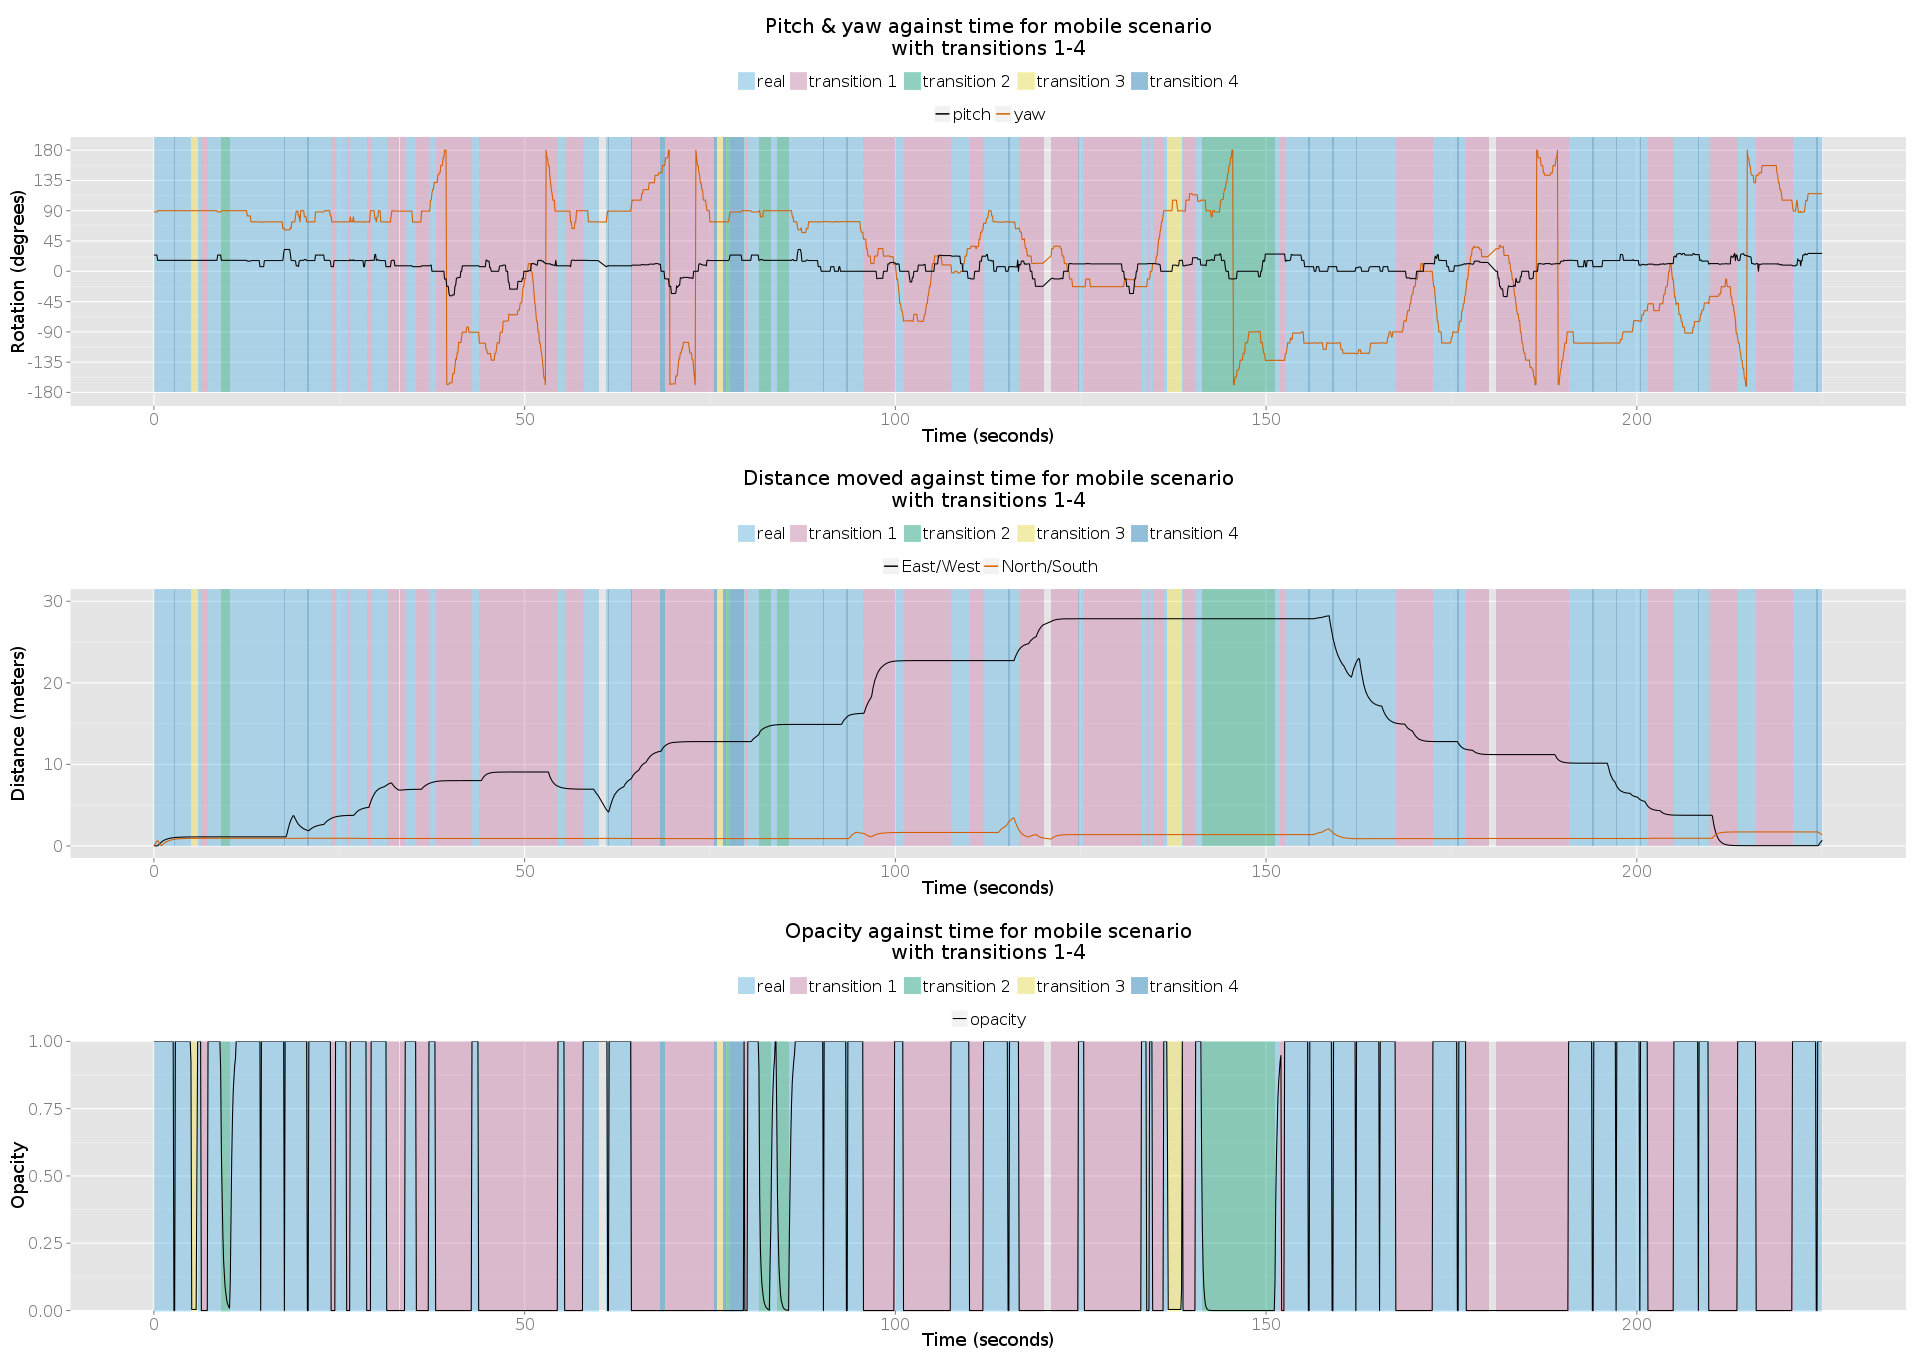
\includegraphics[width=\textwidth]{2.1/8_1-4_3up.png}
	\caption{Some images, yah.}
	\end{center}
\end{figure}

%=========================================================================================================

\clearpage

\subsubsection{Participant 9}

\begin{figure}[h]
	\begin{center}
	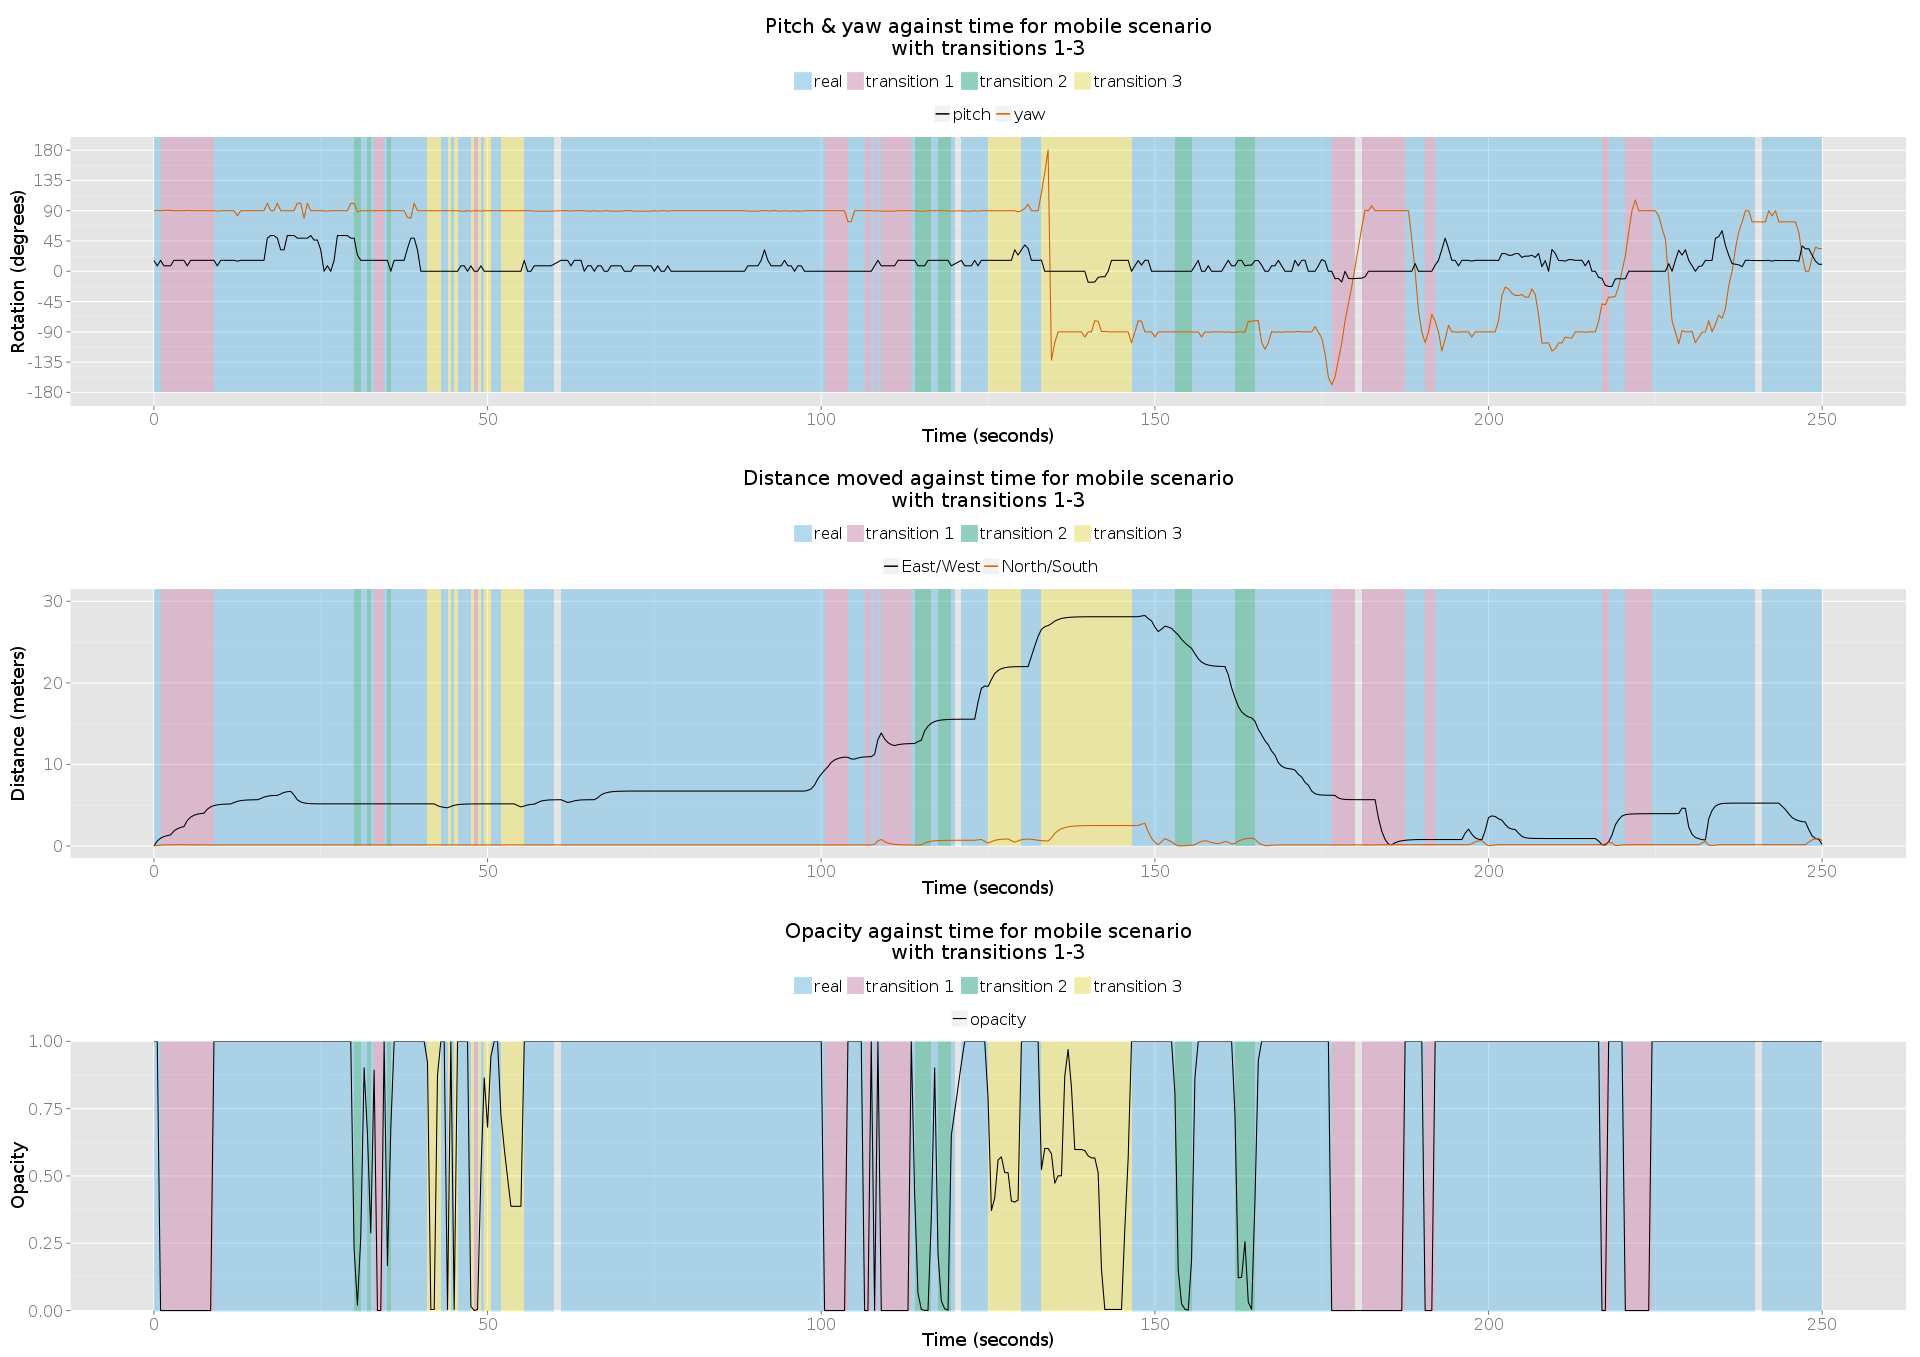
\includegraphics[width=\textwidth]{2.1/9_1-3_3up.png}
	\caption{Some images, yah.}
	\end{center}
\end{figure}

\clearpage

\begin{figure}[h]
	\begin{center}
	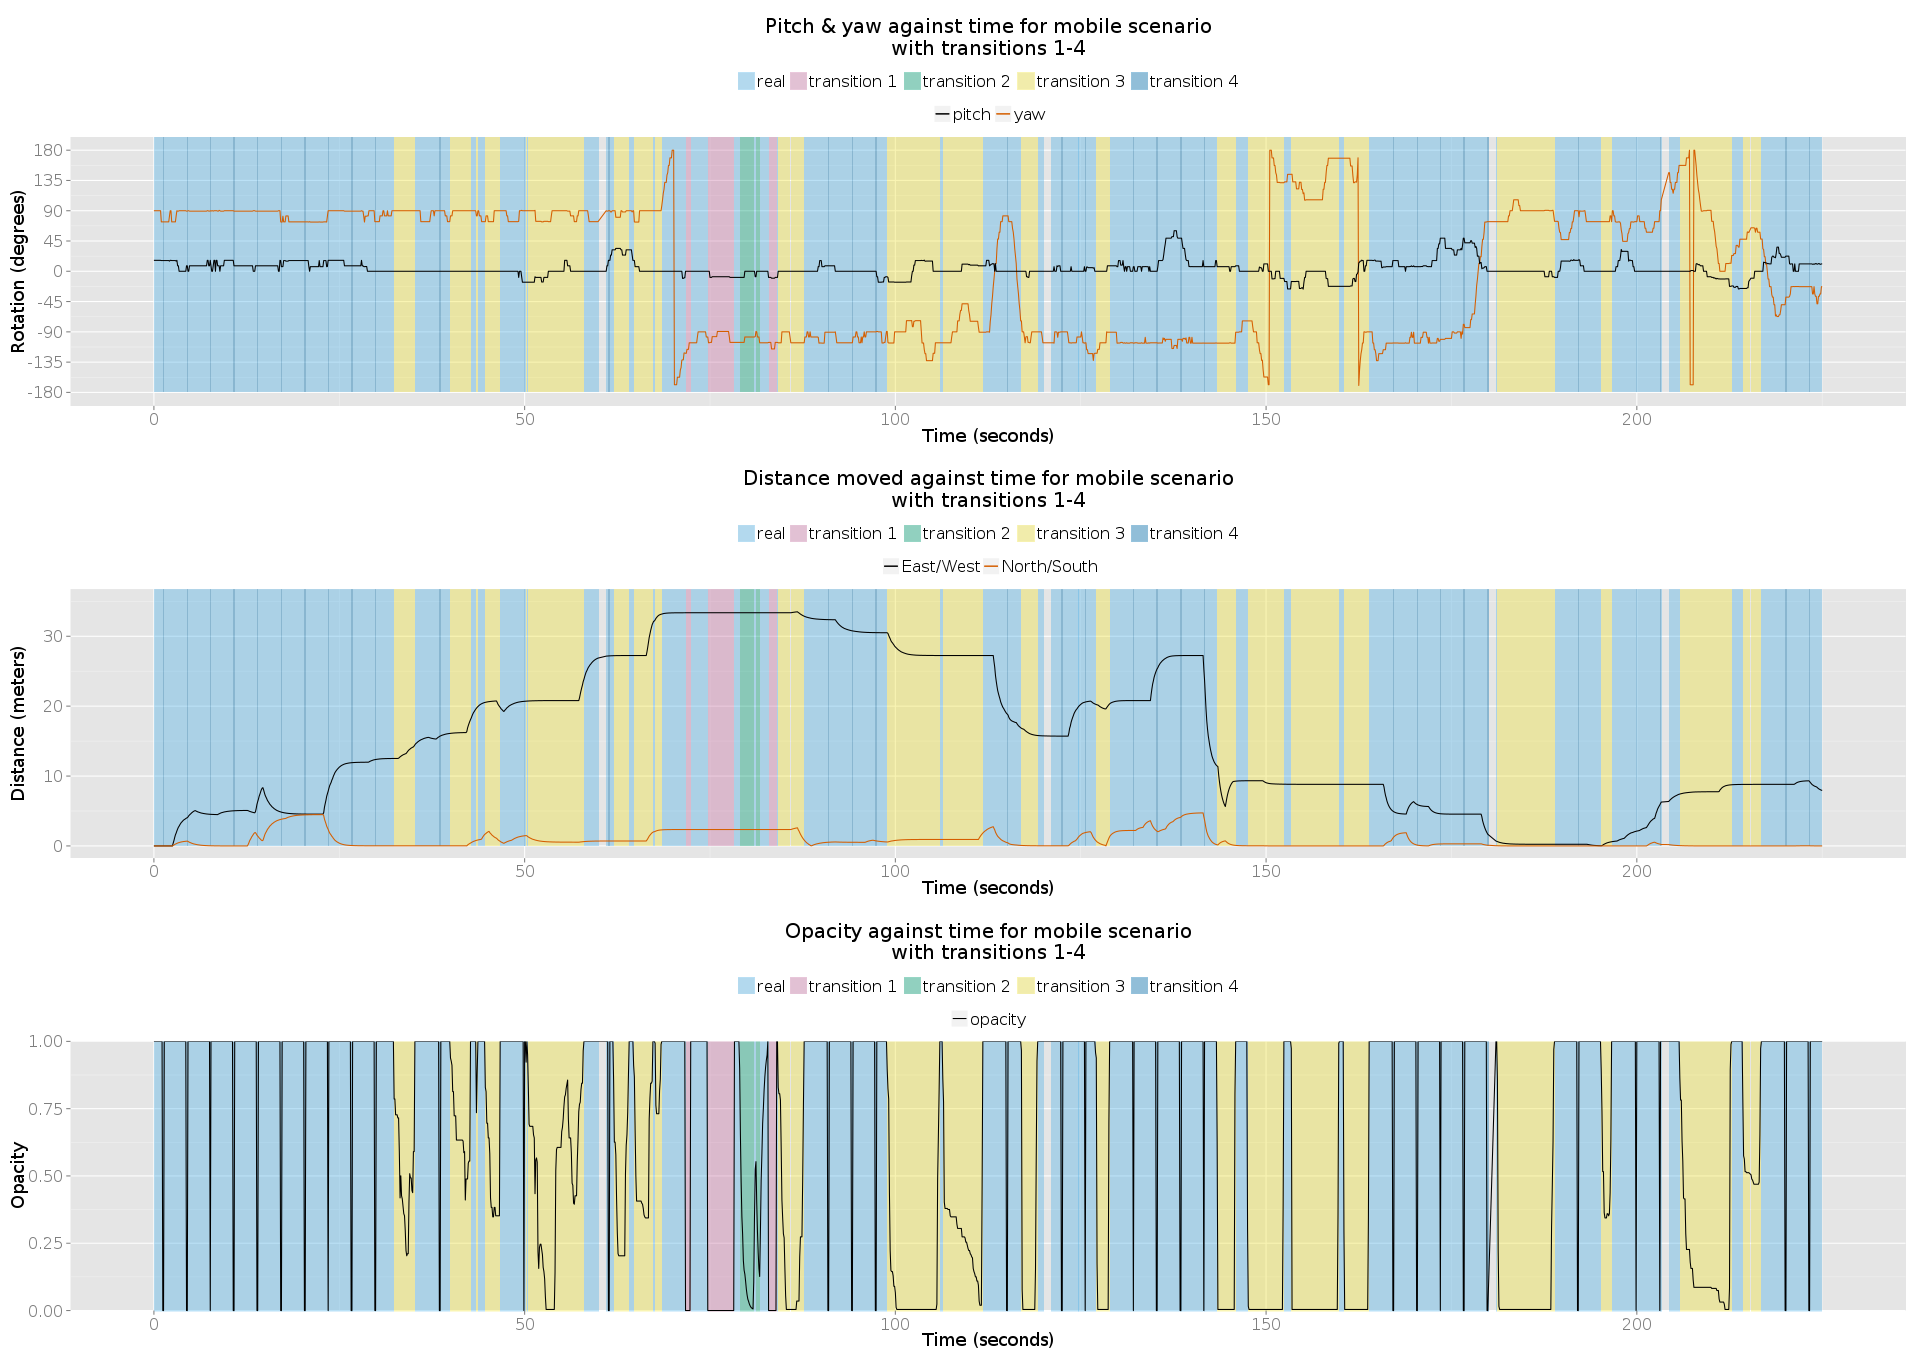
\includegraphics[width=\textwidth]{2.1/9_1-4_3up.png}
	\caption{Some images, yah.}
	\end{center}
\end{figure}

%=========================================================================================================

\clearpage

\subsubsection{Participant 10}

\begin{figure}[h]
	\begin{center}
	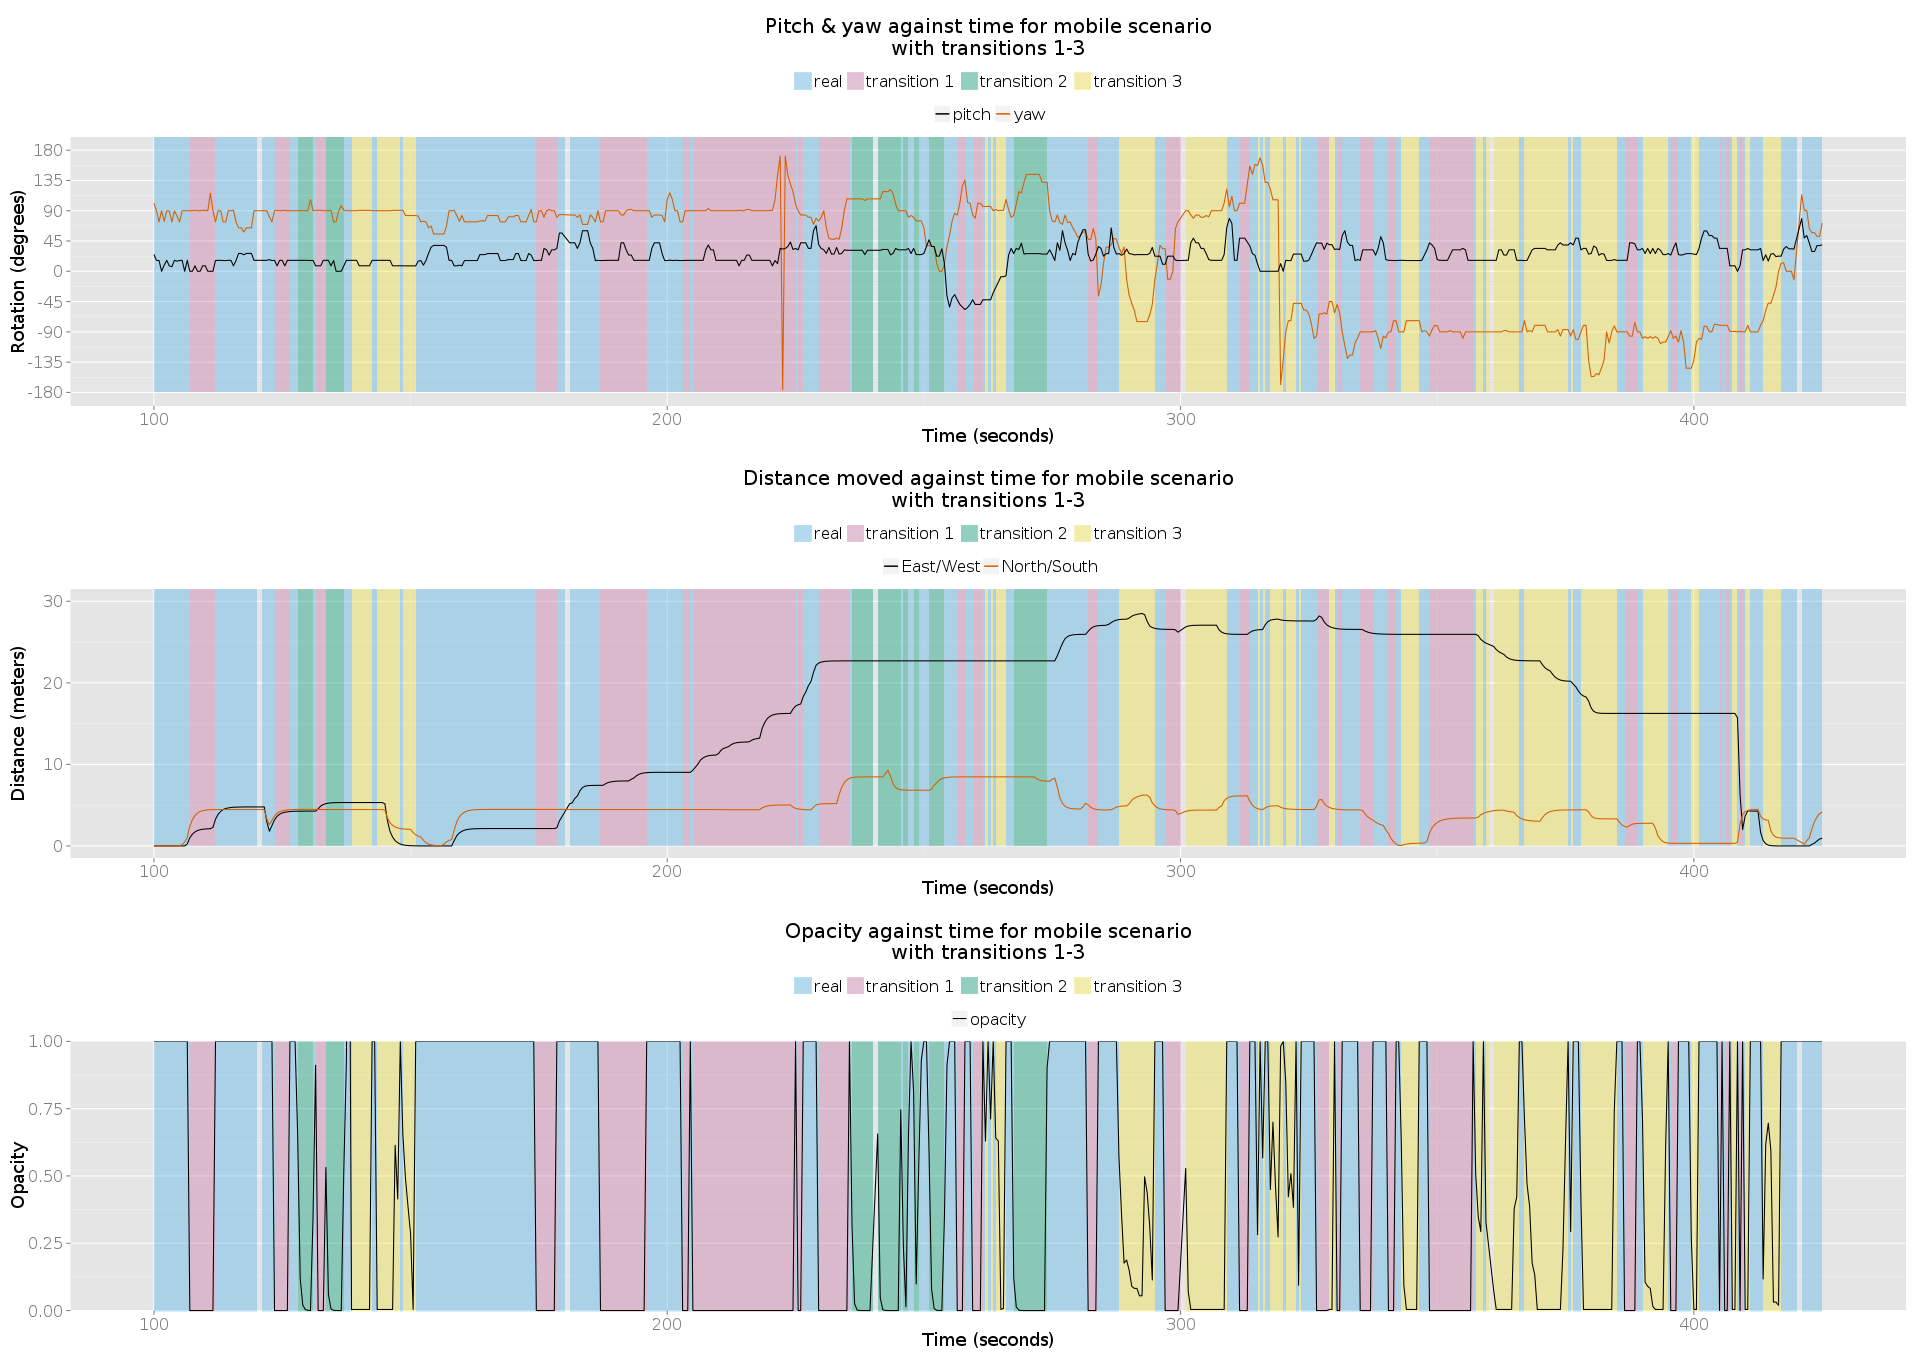
\includegraphics[width=\textwidth]{2.1/10_1-3_3up.png}
	\caption{Some images, yah.}
	\end{center}
\end{figure}

\clearpage

\begin{figure}[h]
	\begin{center}
	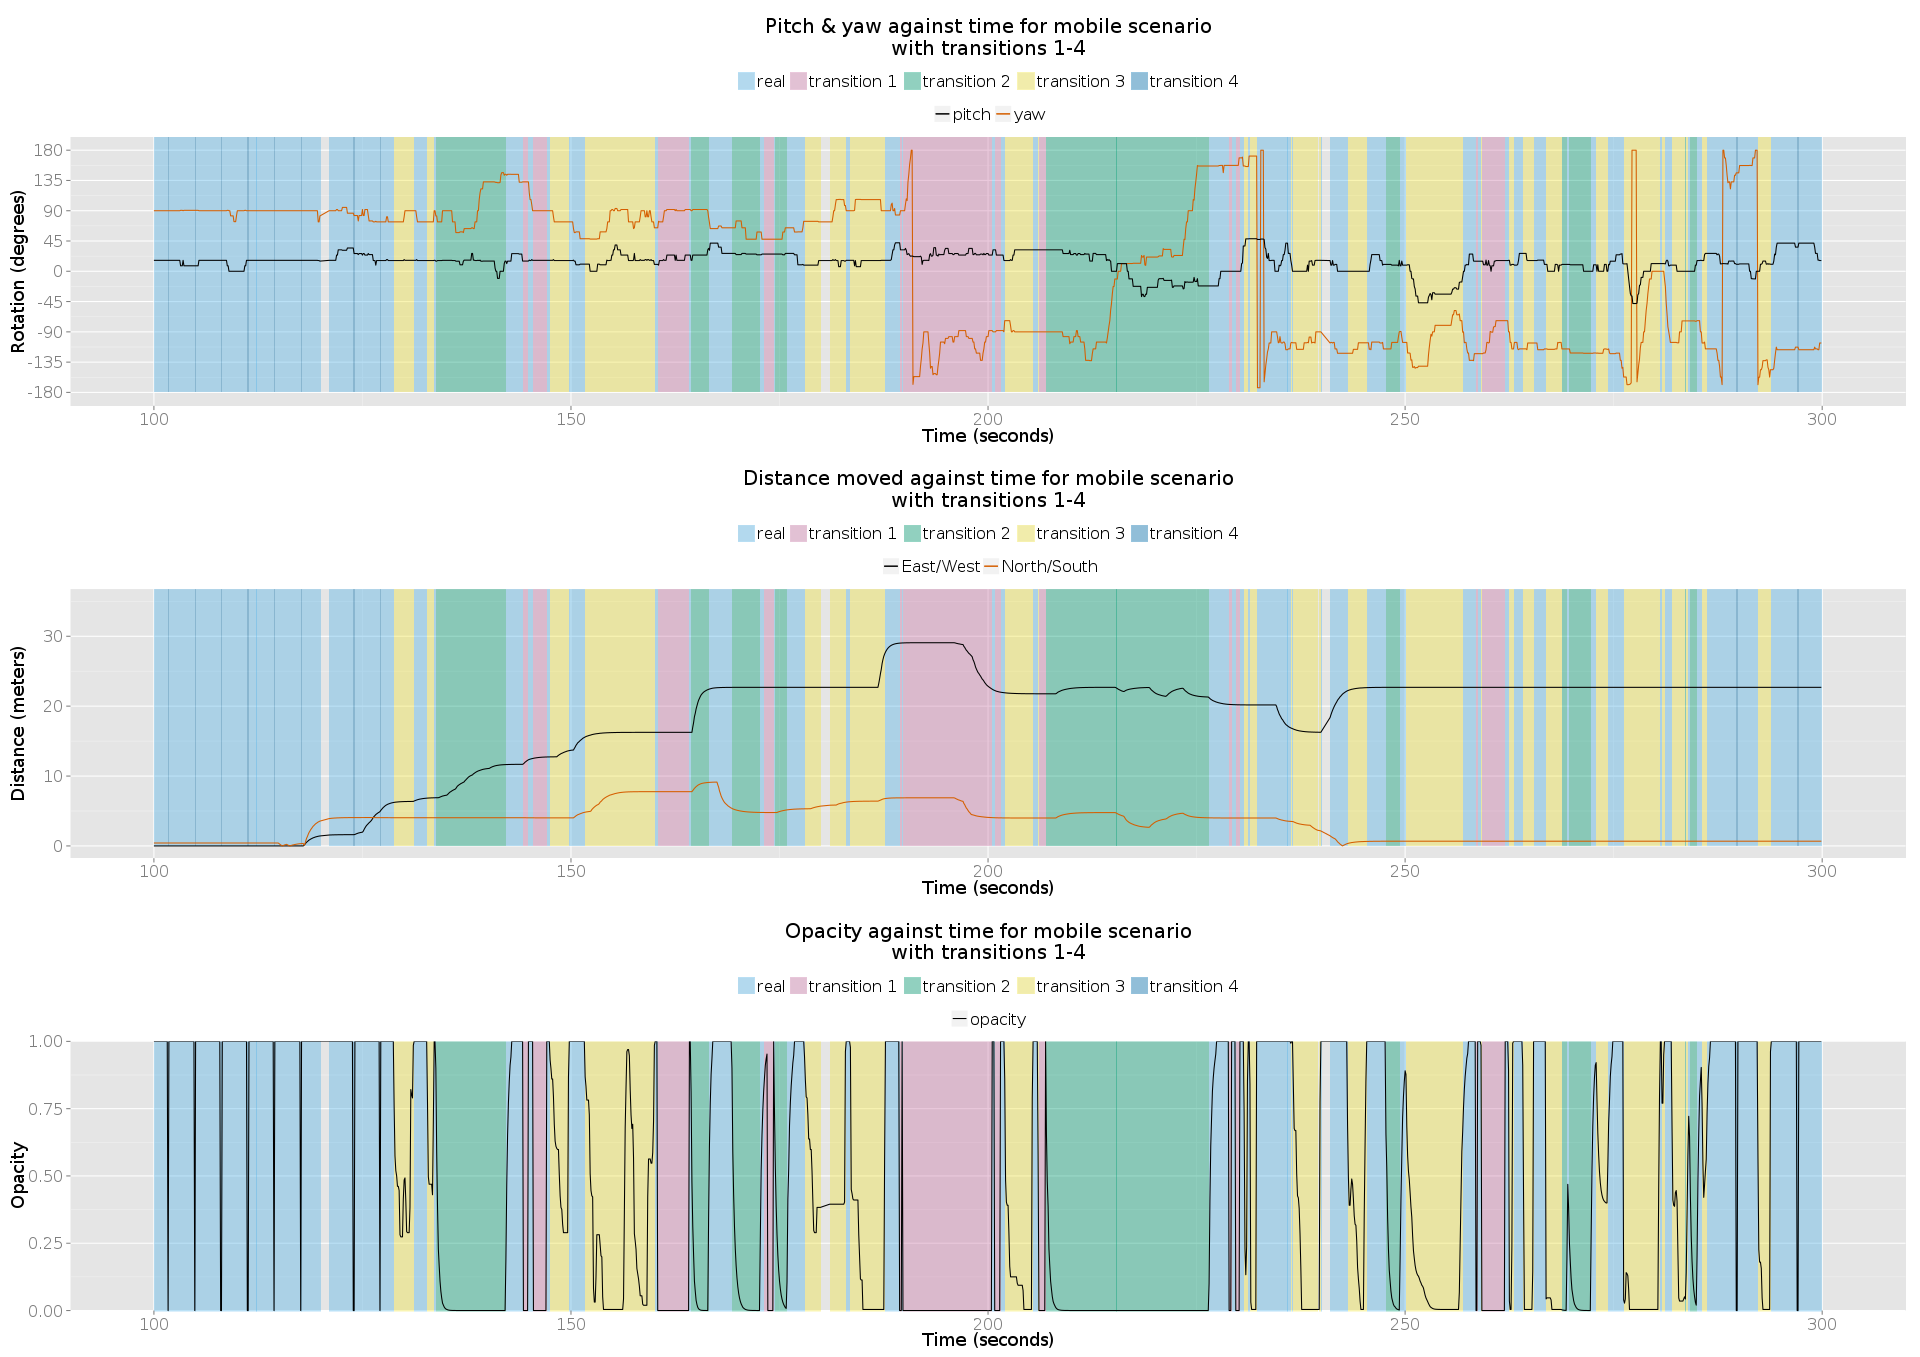
\includegraphics[width=\textwidth]{2.1/10_1-4_3up.png}
	\caption{Some images, yah.}
	\end{center}
\end{figure}

%=========================================================================================================

\clearpage

\subsubsection{Participant 11}

\begin{figure}[h]
	\begin{center}
	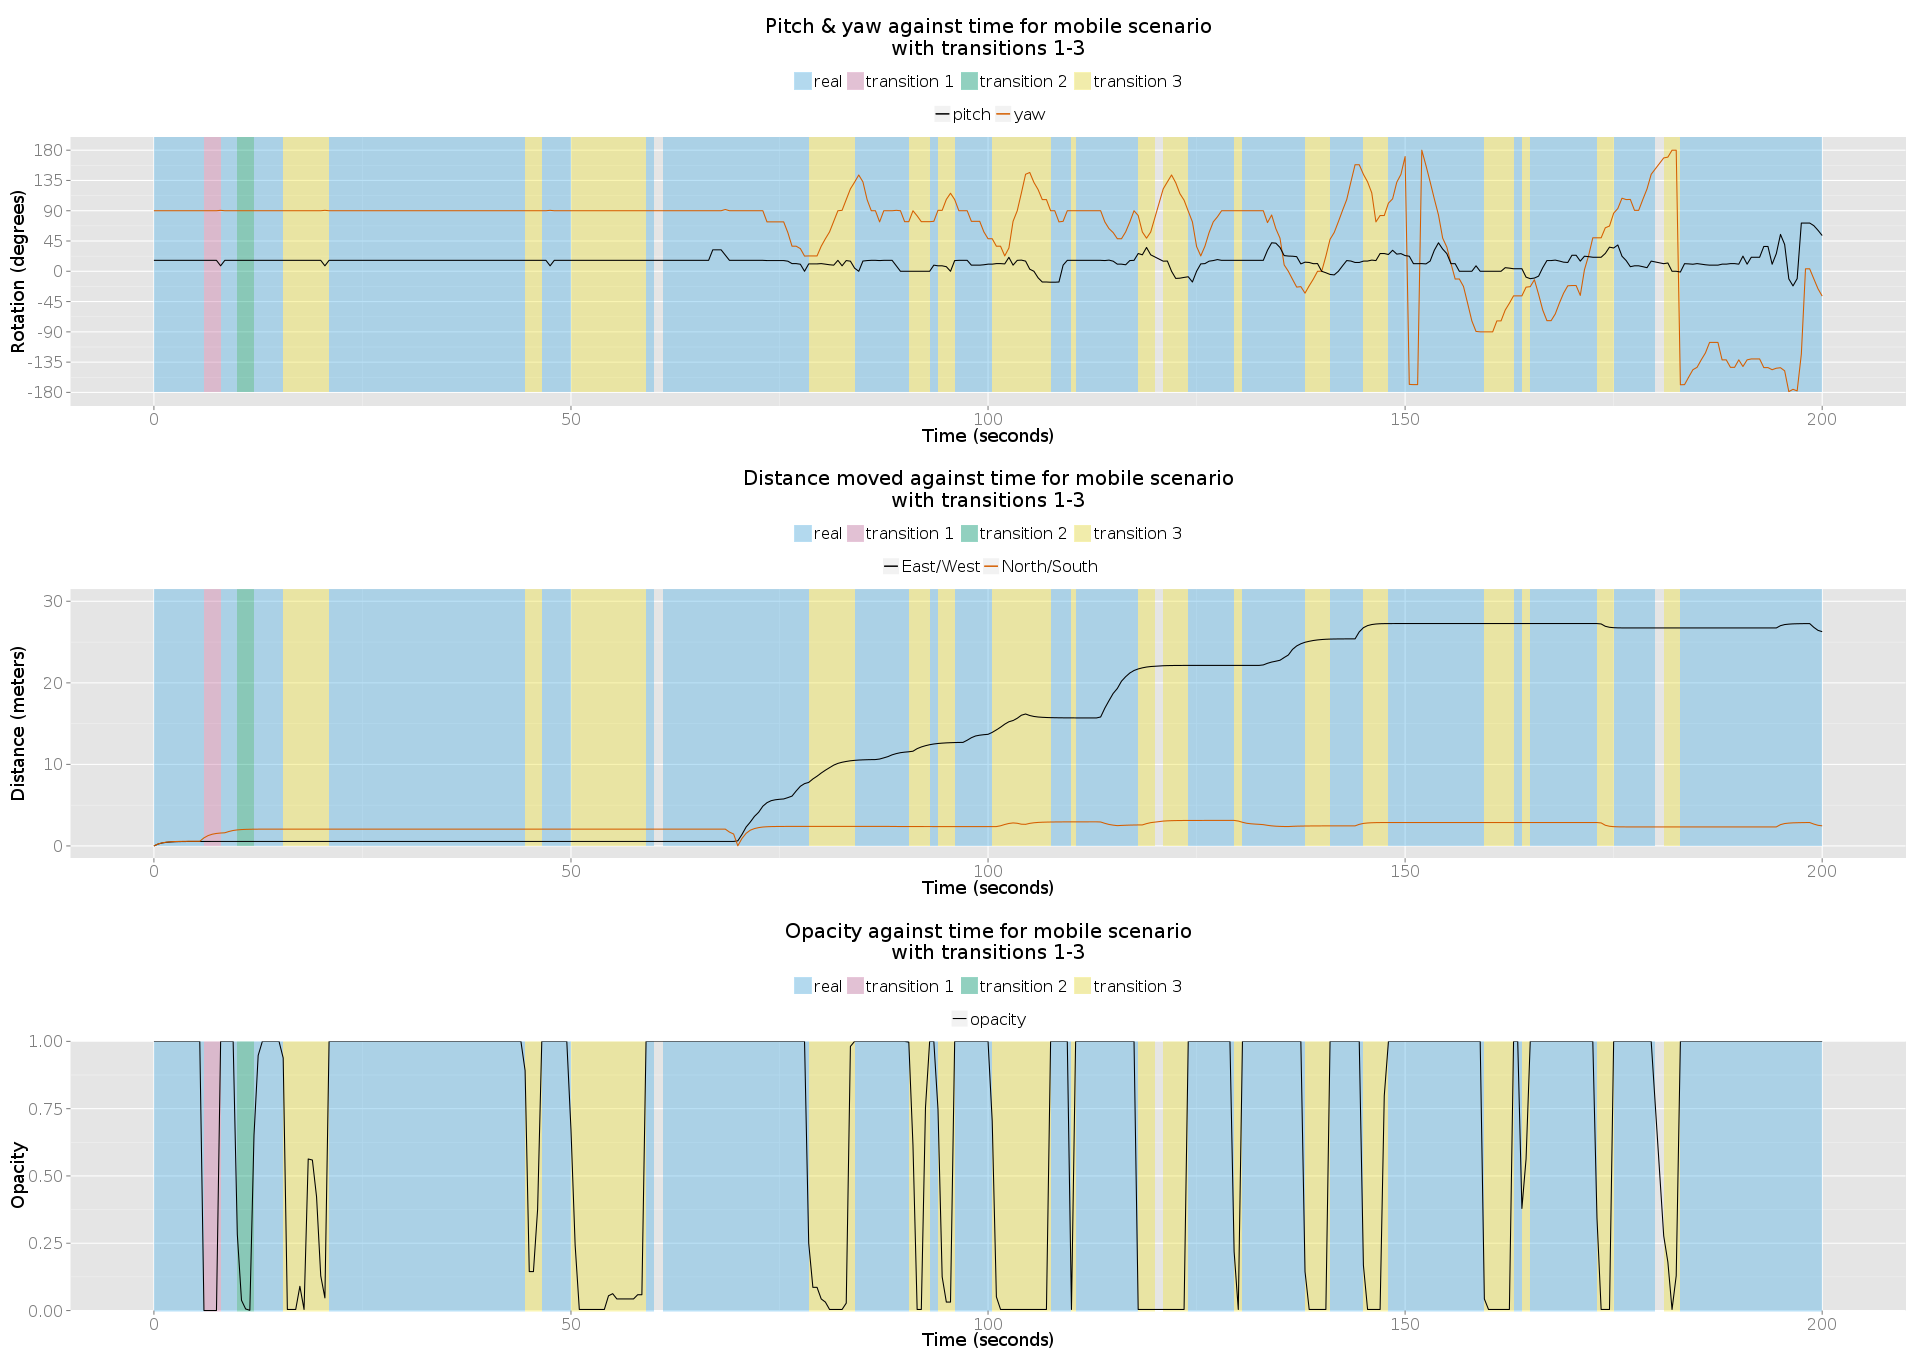
\includegraphics[width=\textwidth]{2.1/11_1-3_3up.png}
	\caption{Some images, yah.}
	\end{center}
\end{figure}

\clearpage

\begin{figure}[h]
	\begin{center}
	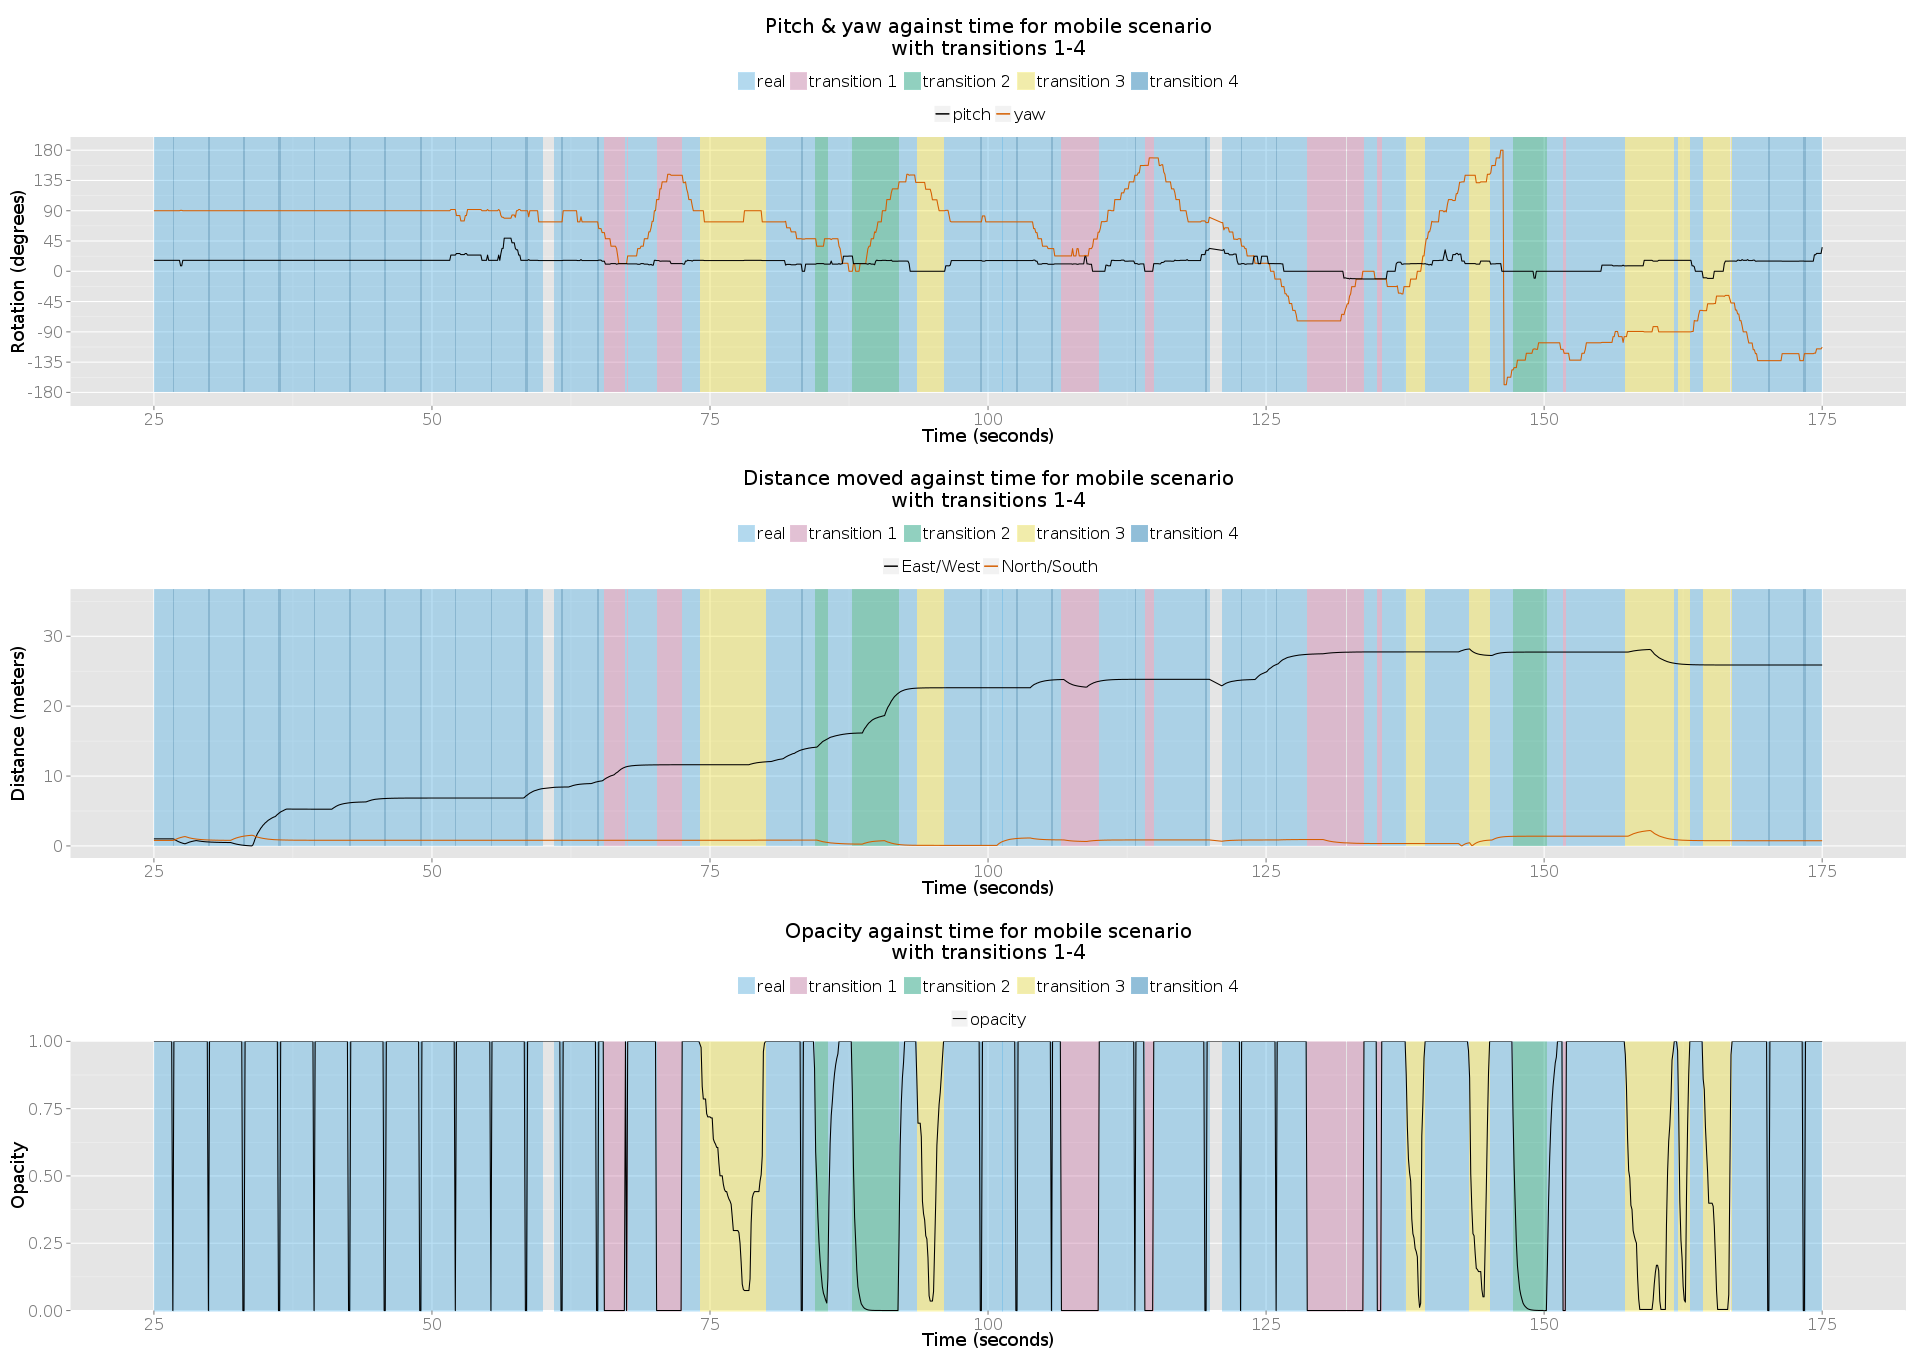
\includegraphics[width=\textwidth]{2.1/11_1-4_3up.png}
	\caption{Some images, yah.}
	\end{center}
\end{figure}

%=========================================================================================================

\clearpage

\subsubsection{Participant 12}

\begin{figure}[h]
	\begin{center}
	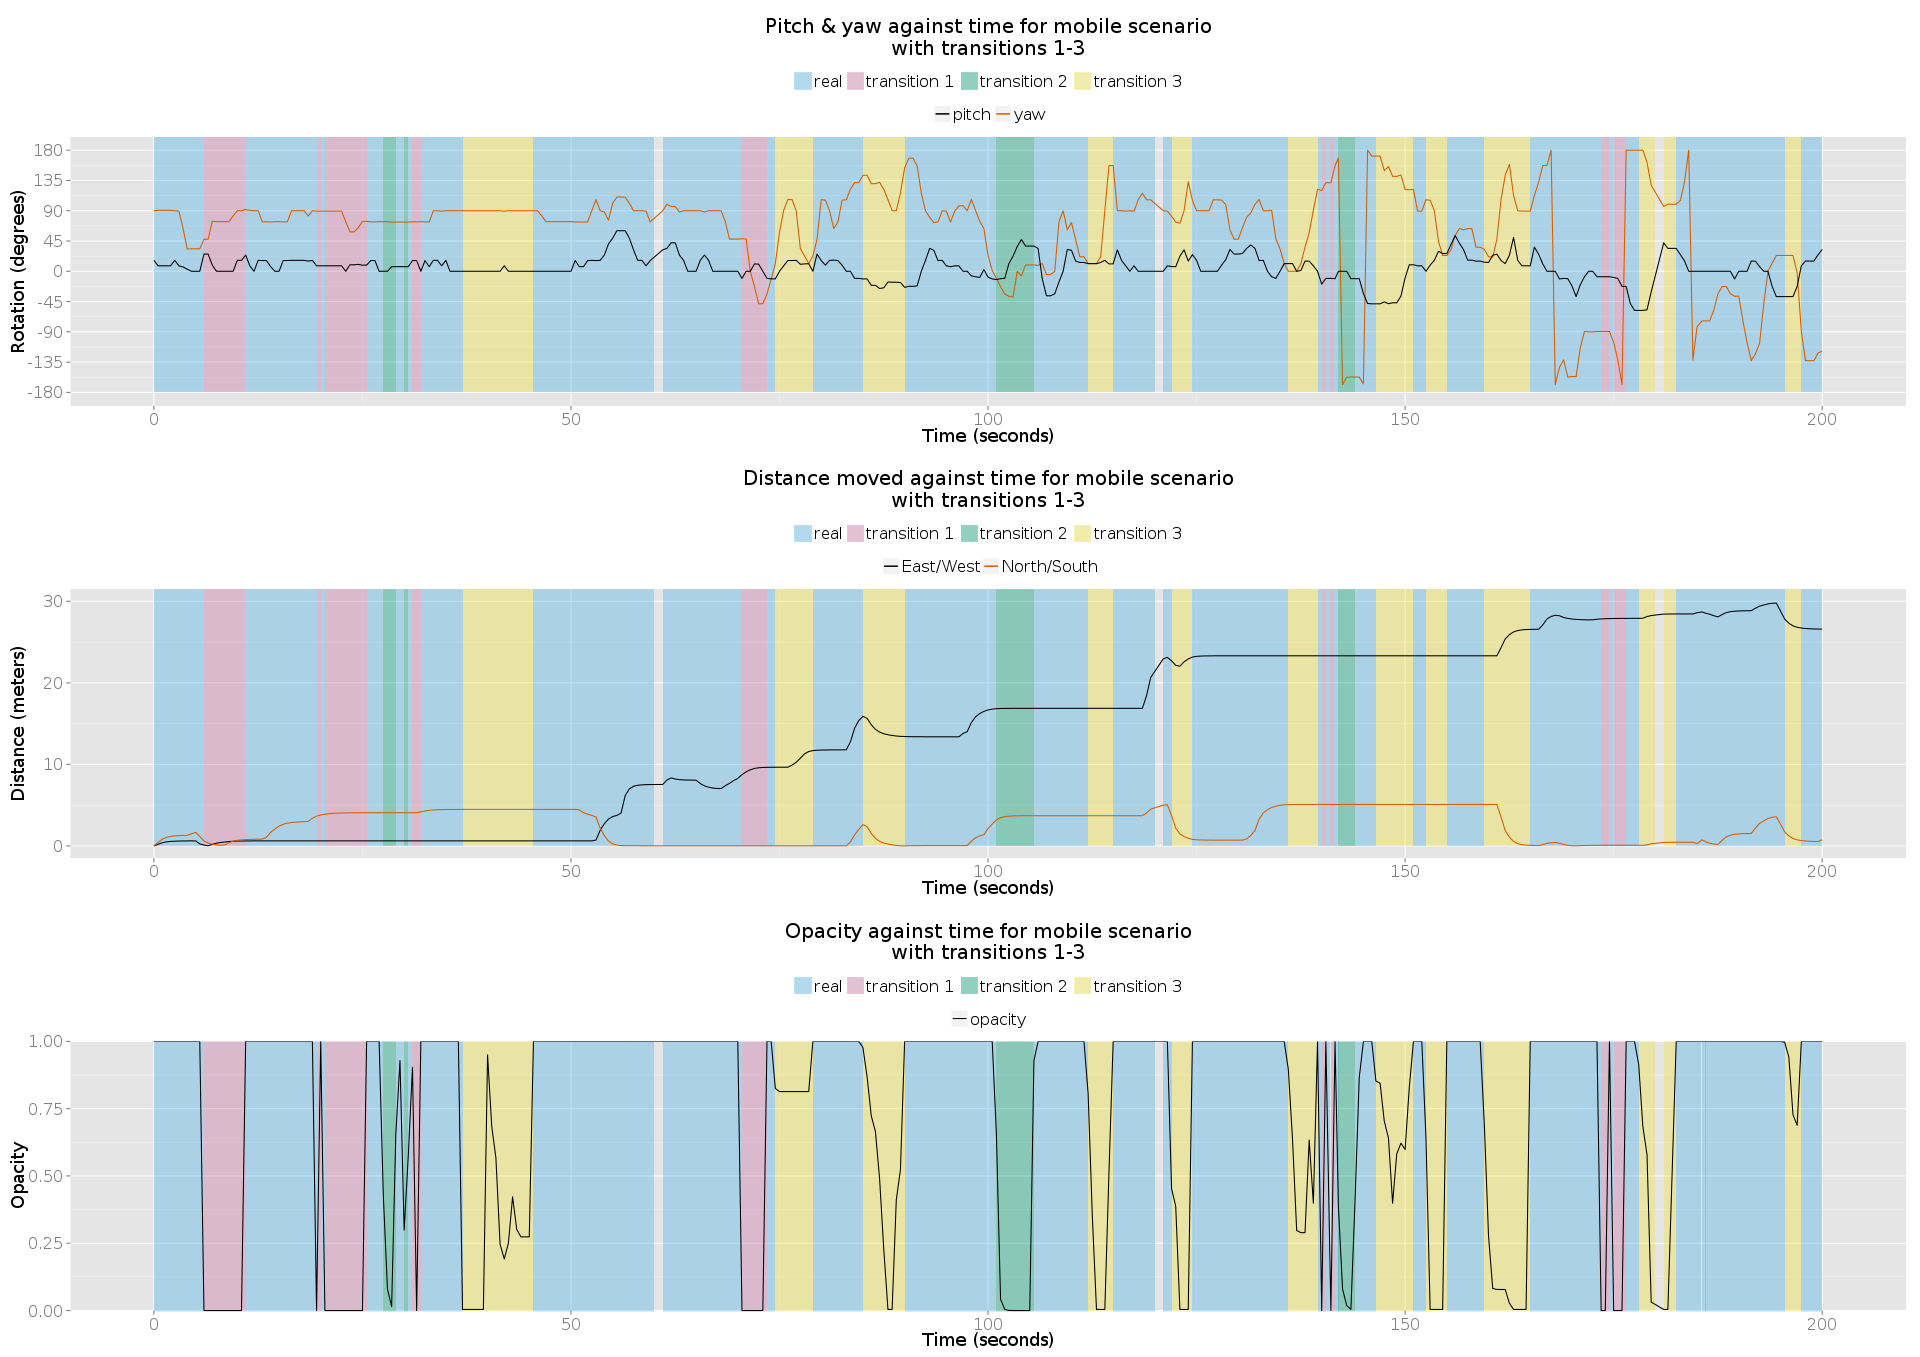
\includegraphics[width=\textwidth]{2.1/12_1-3_3up.png}
	\caption{Some images, yah.}
	\end{center}
\end{figure}

\clearpage

\begin{figure}[h]
	\begin{center}
	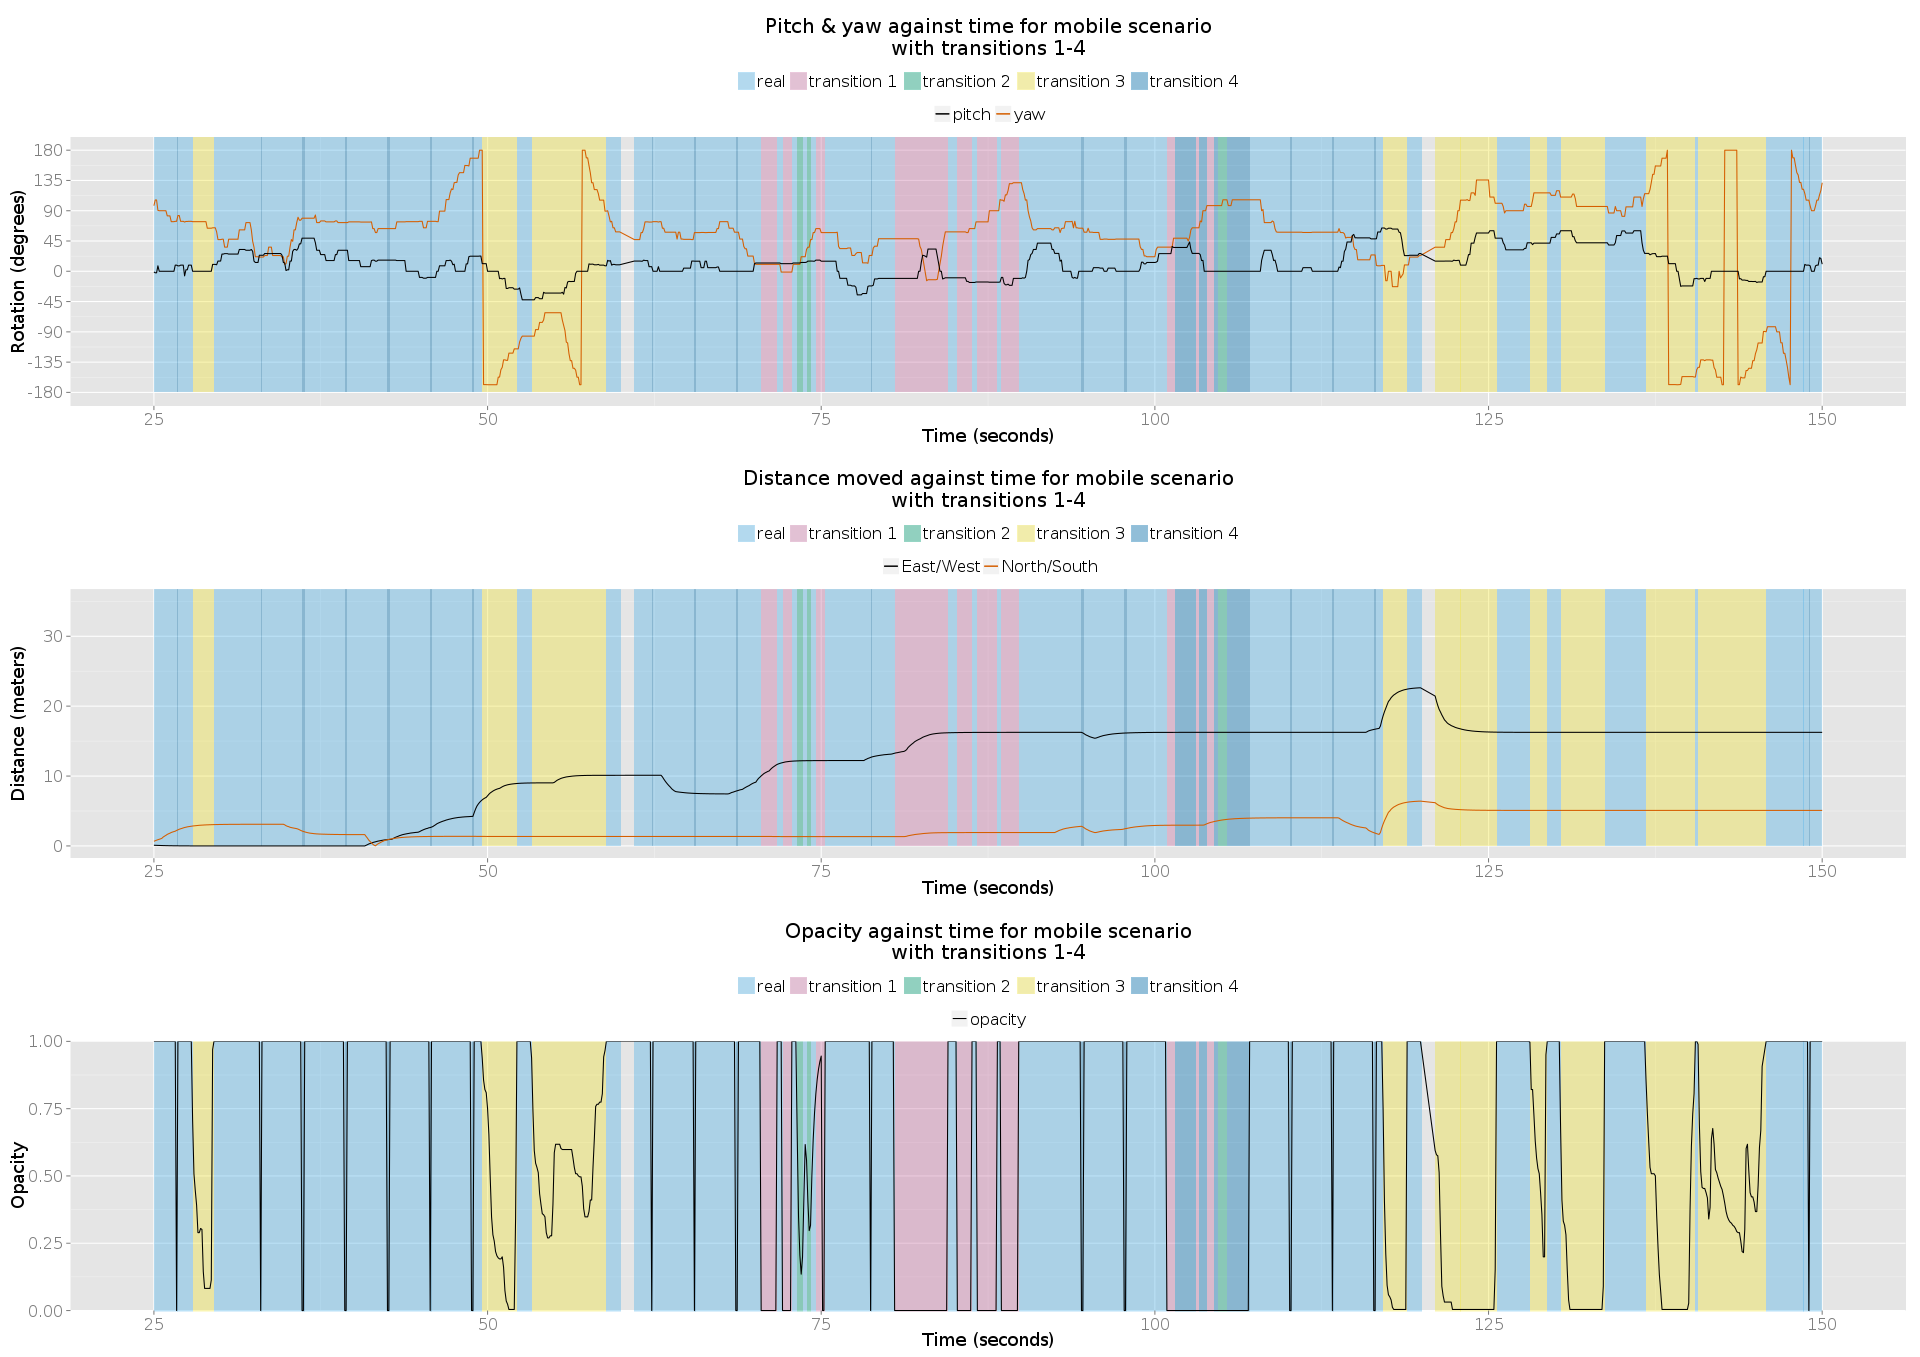
\includegraphics[width=\textwidth]{2.1/12_1-4_3up.png}
	\caption{Some images, yah.}
	\end{center}
\end{figure}

%=========================================================================================================

\clearpage

\subsubsection{Participant 13}

\begin{figure}[h]
	\begin{center}
	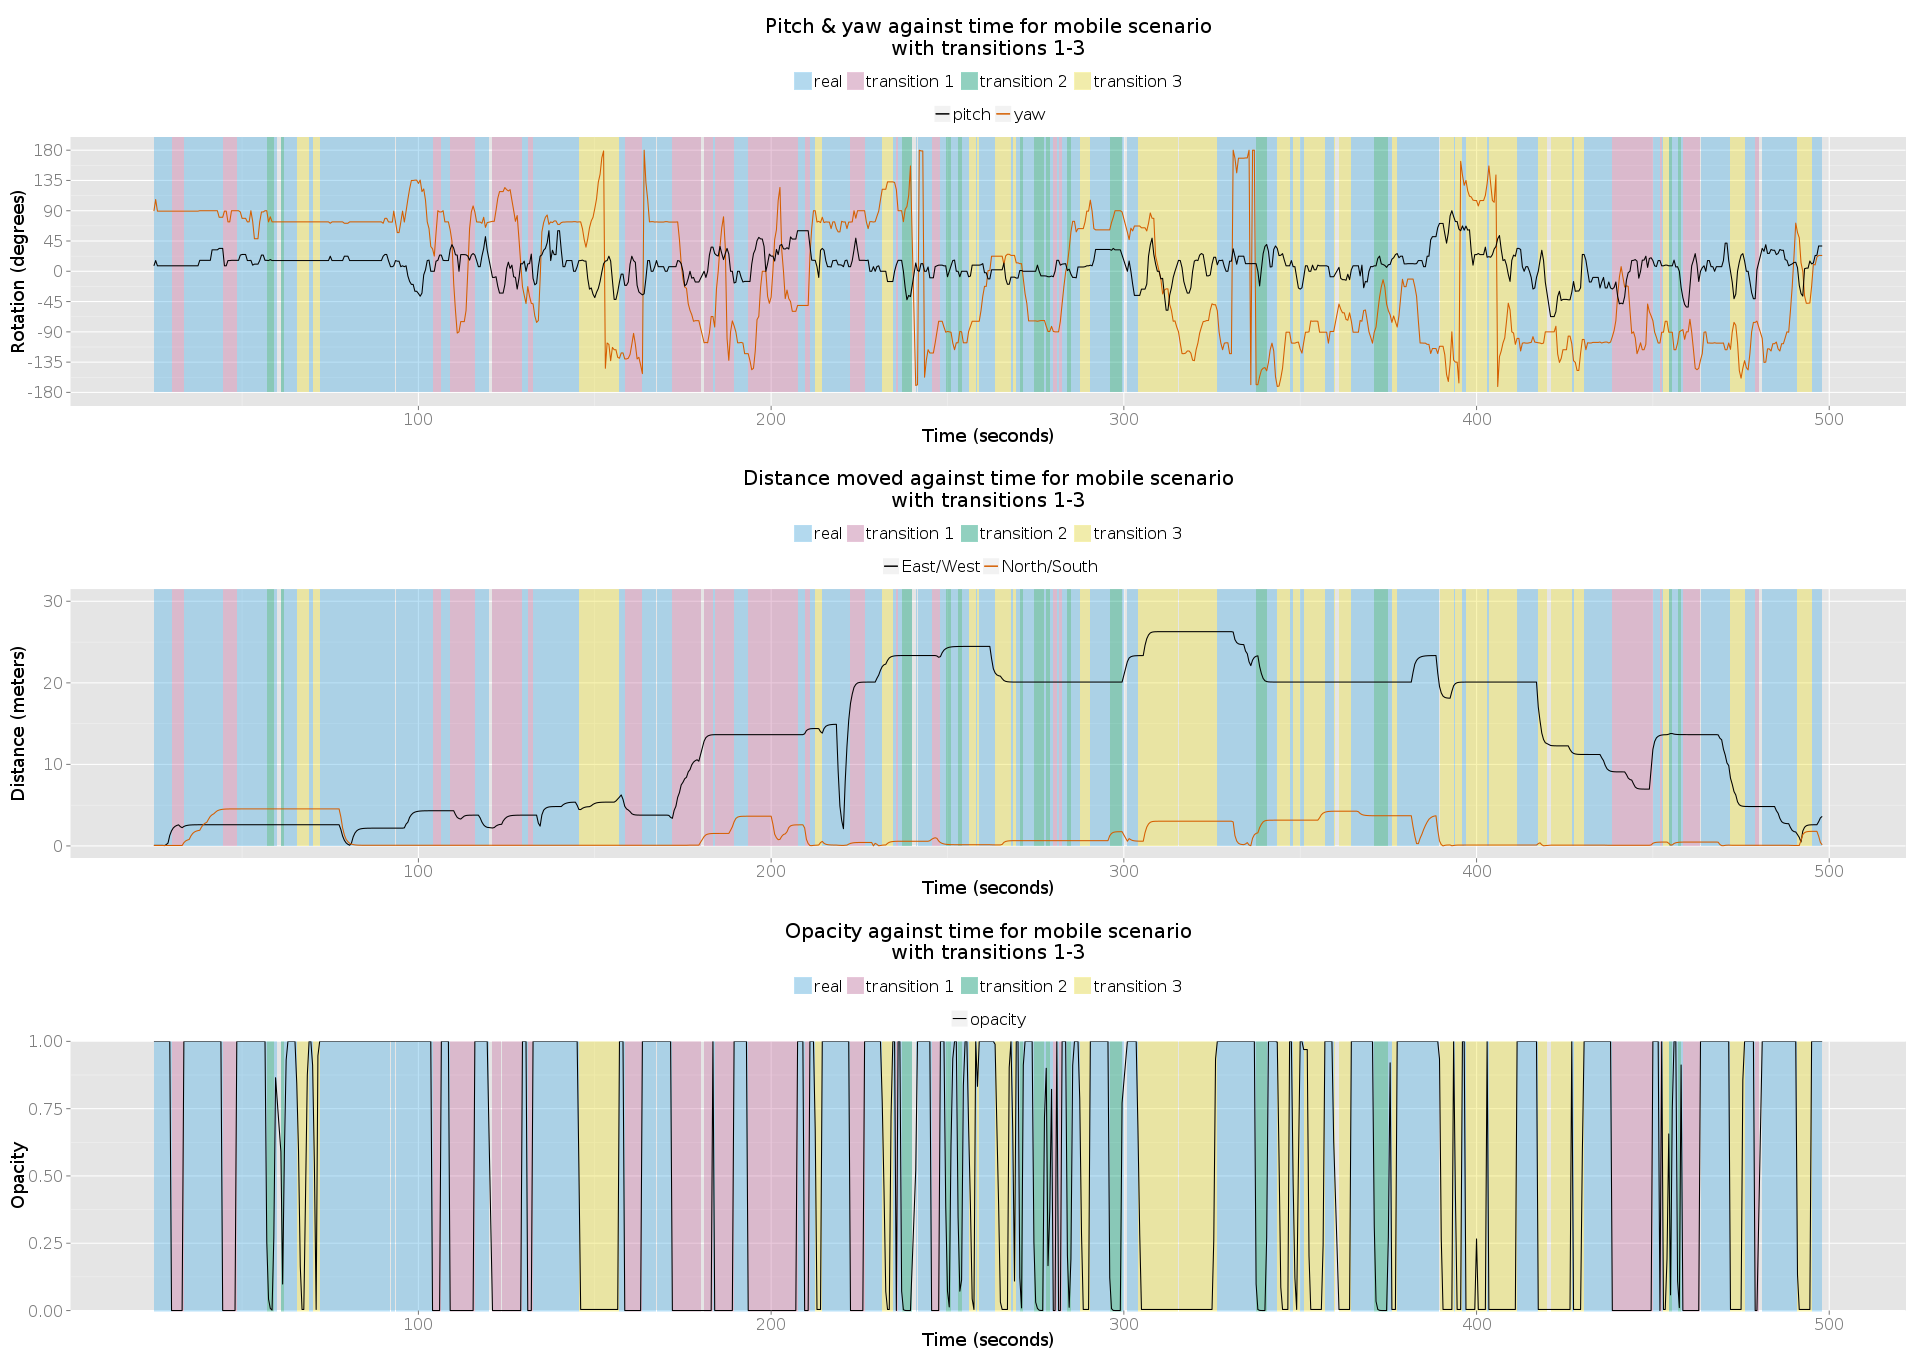
\includegraphics[width=\textwidth]{2.1/13_1-3_3up.png}
	\caption{Some images, yah.}
	\end{center}
\end{figure}

\clearpage

\begin{figure}[h]
	\begin{center}
	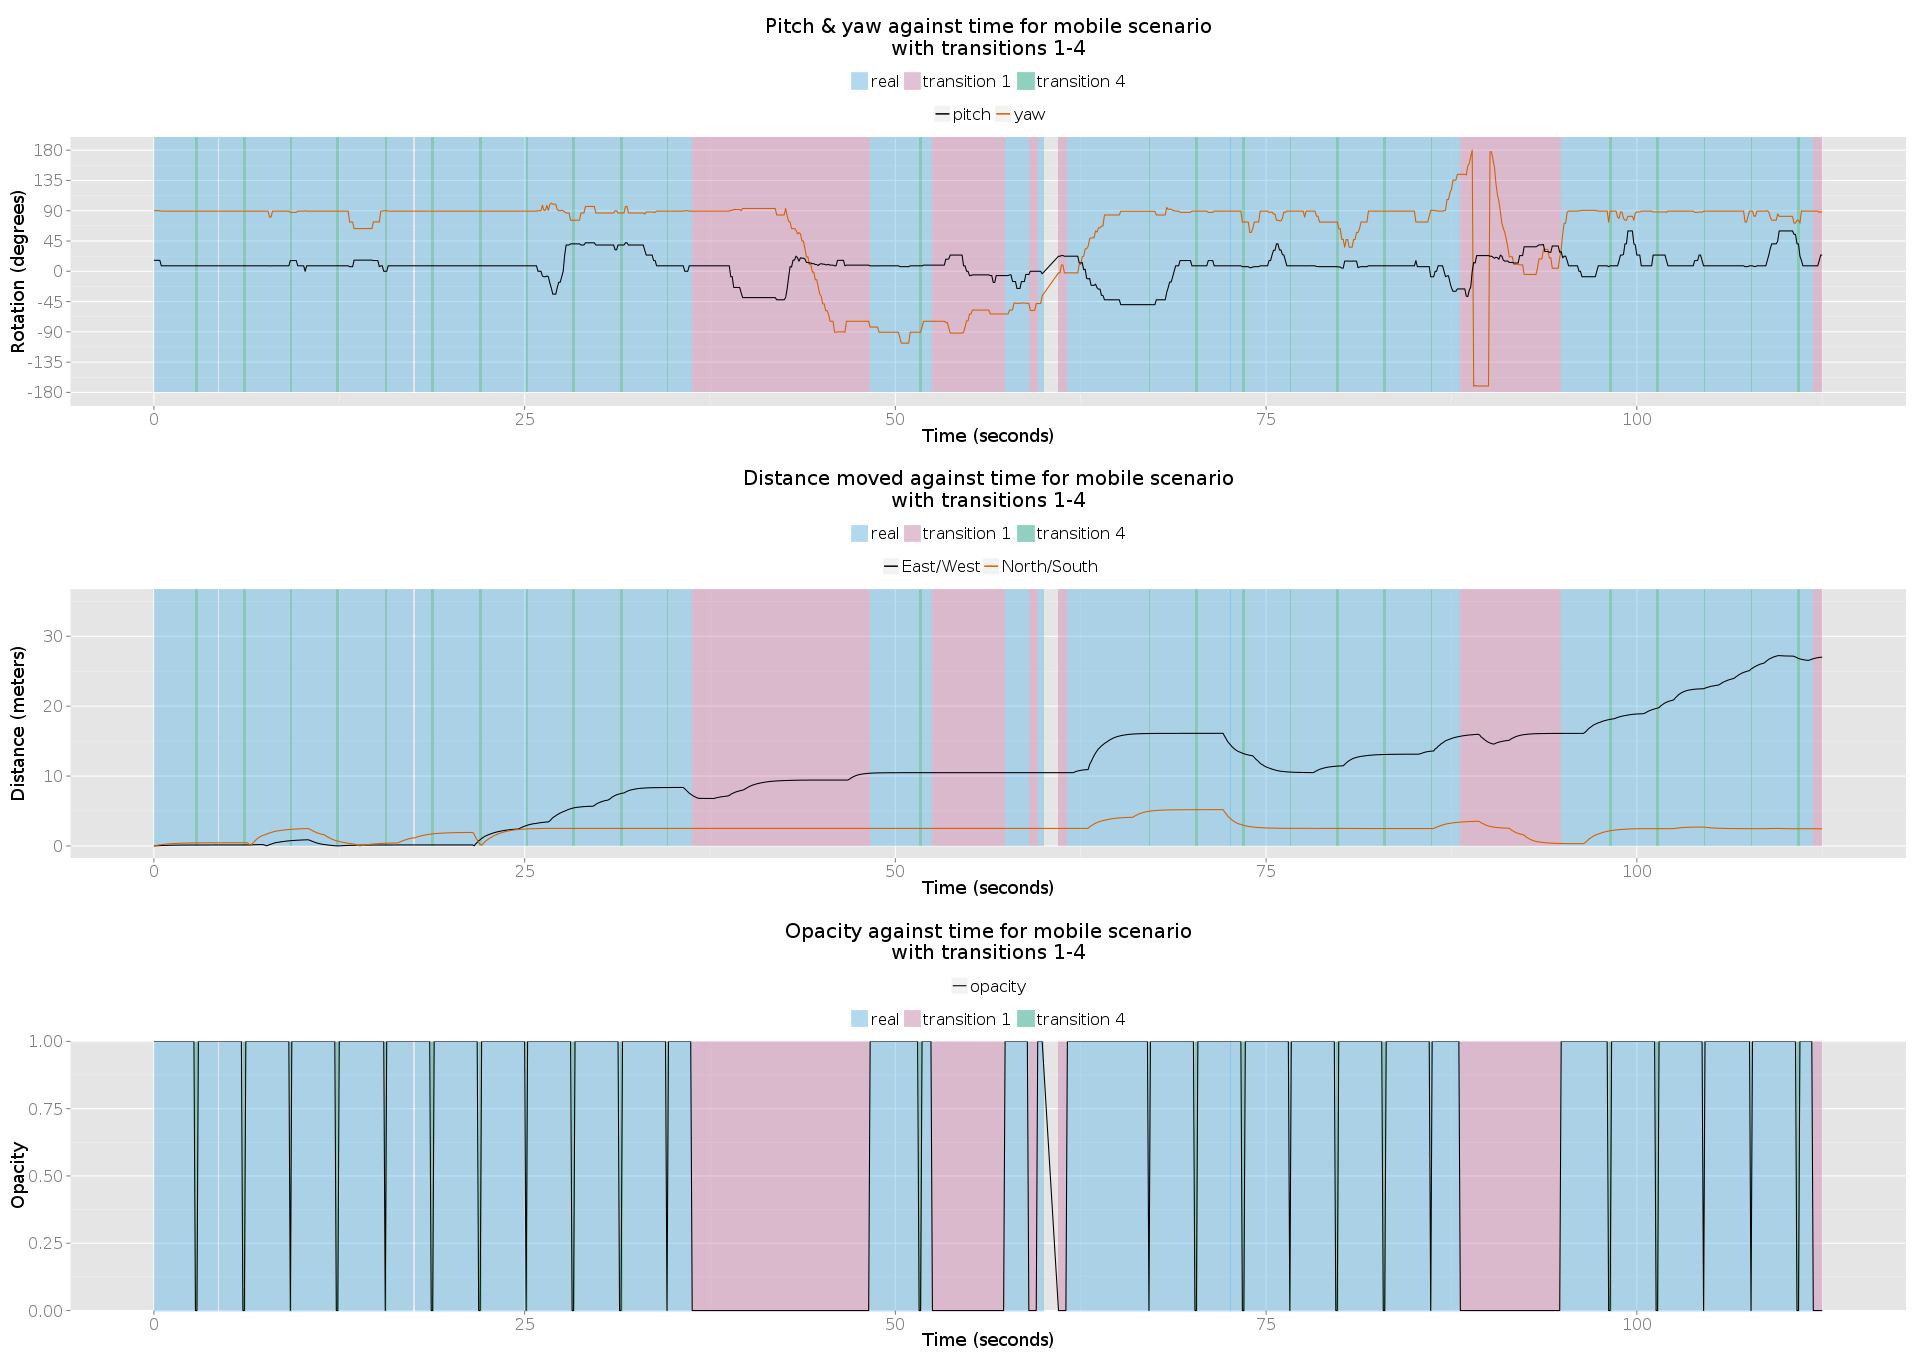
\includegraphics[width=\textwidth]{2.1/13_1-4_3up.png}
	\caption{Some images, yah.}
	\end{center}
\end{figure}

%=========================================================================================================

\section{Stage 2.1 Conclusions}

%=========================================================================================================

\clearpage

%=========================================================================================================

\section{Phase 2.2 Results}

%=========================================================================================================

\clearpage

\subsubsection{Participant 14}

\begin{figure}[h]
	\begin{center}
	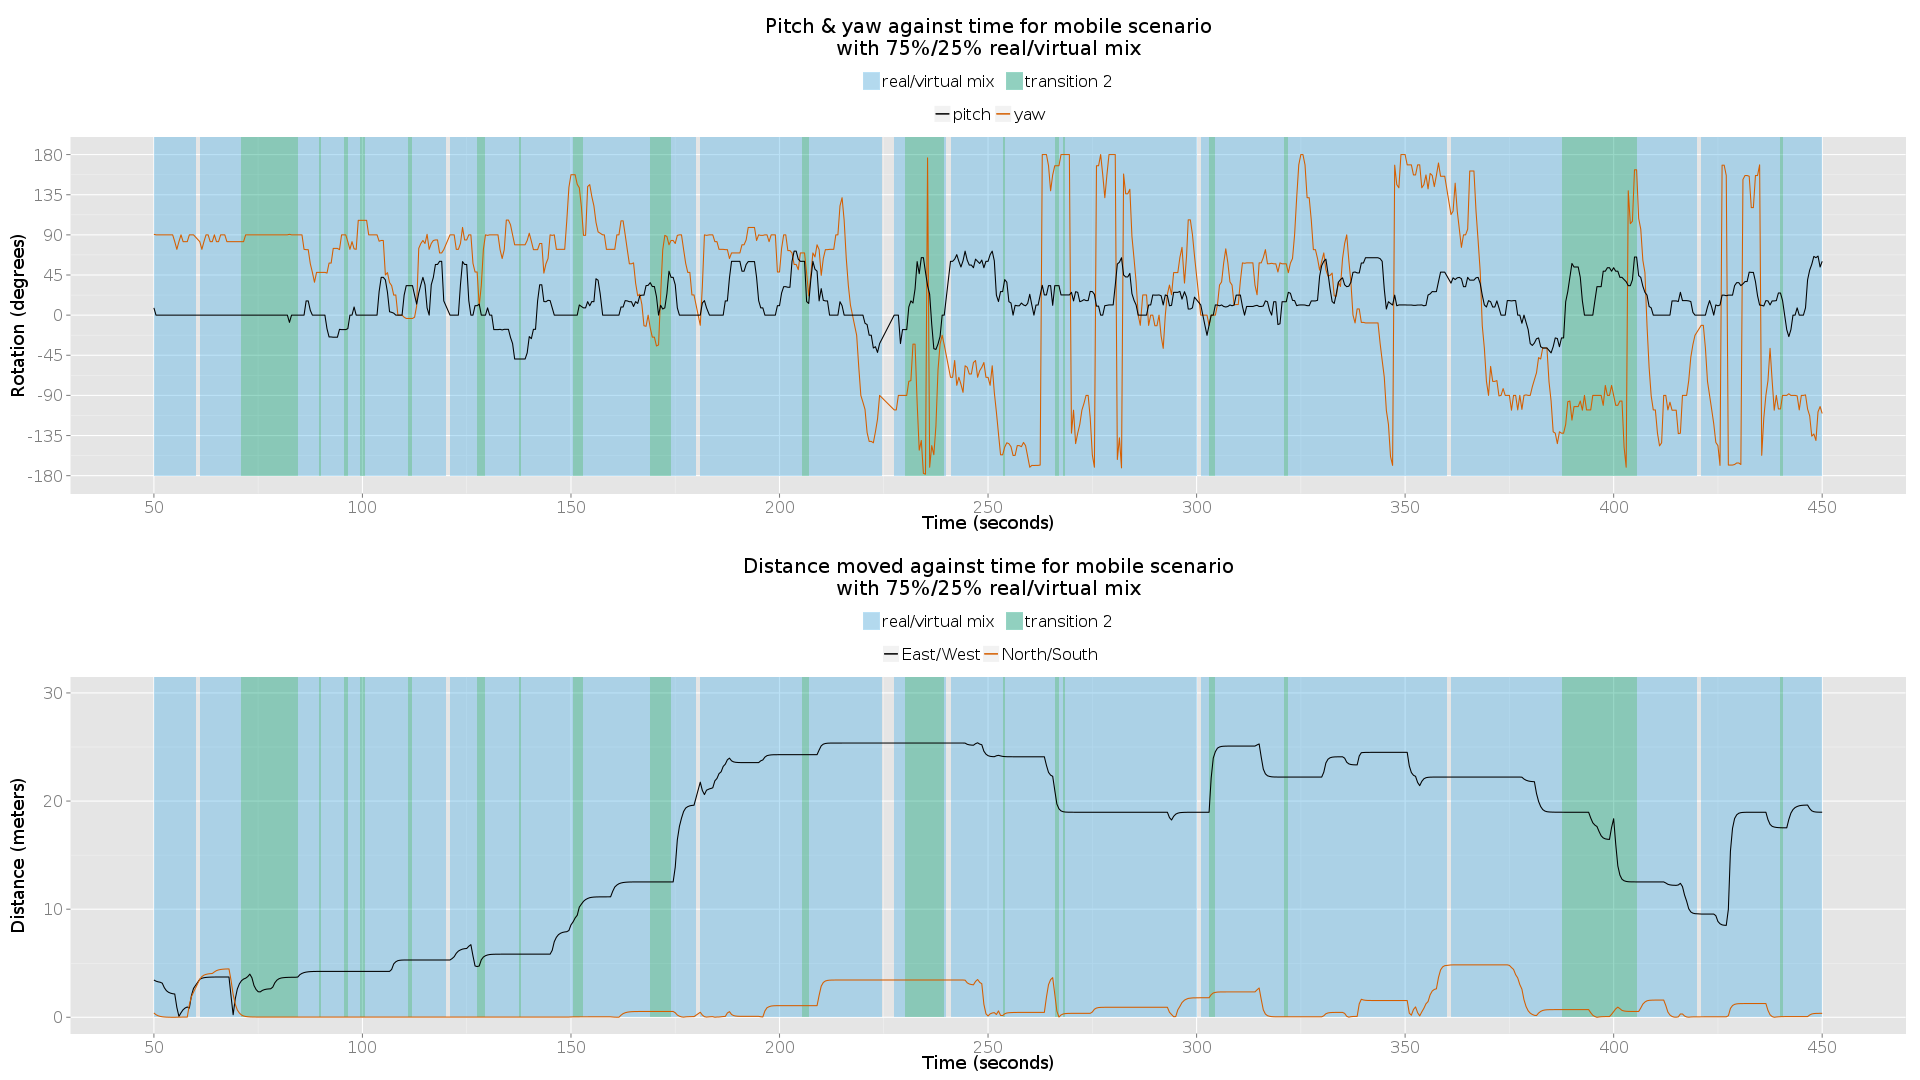
\includegraphics[width=\textwidth]{2.2/14_75_2up.png}
	\caption{Some images, yah.}
	\end{center}
\end{figure}

\clearpage

\begin{figure}[h]
	\begin{center}
	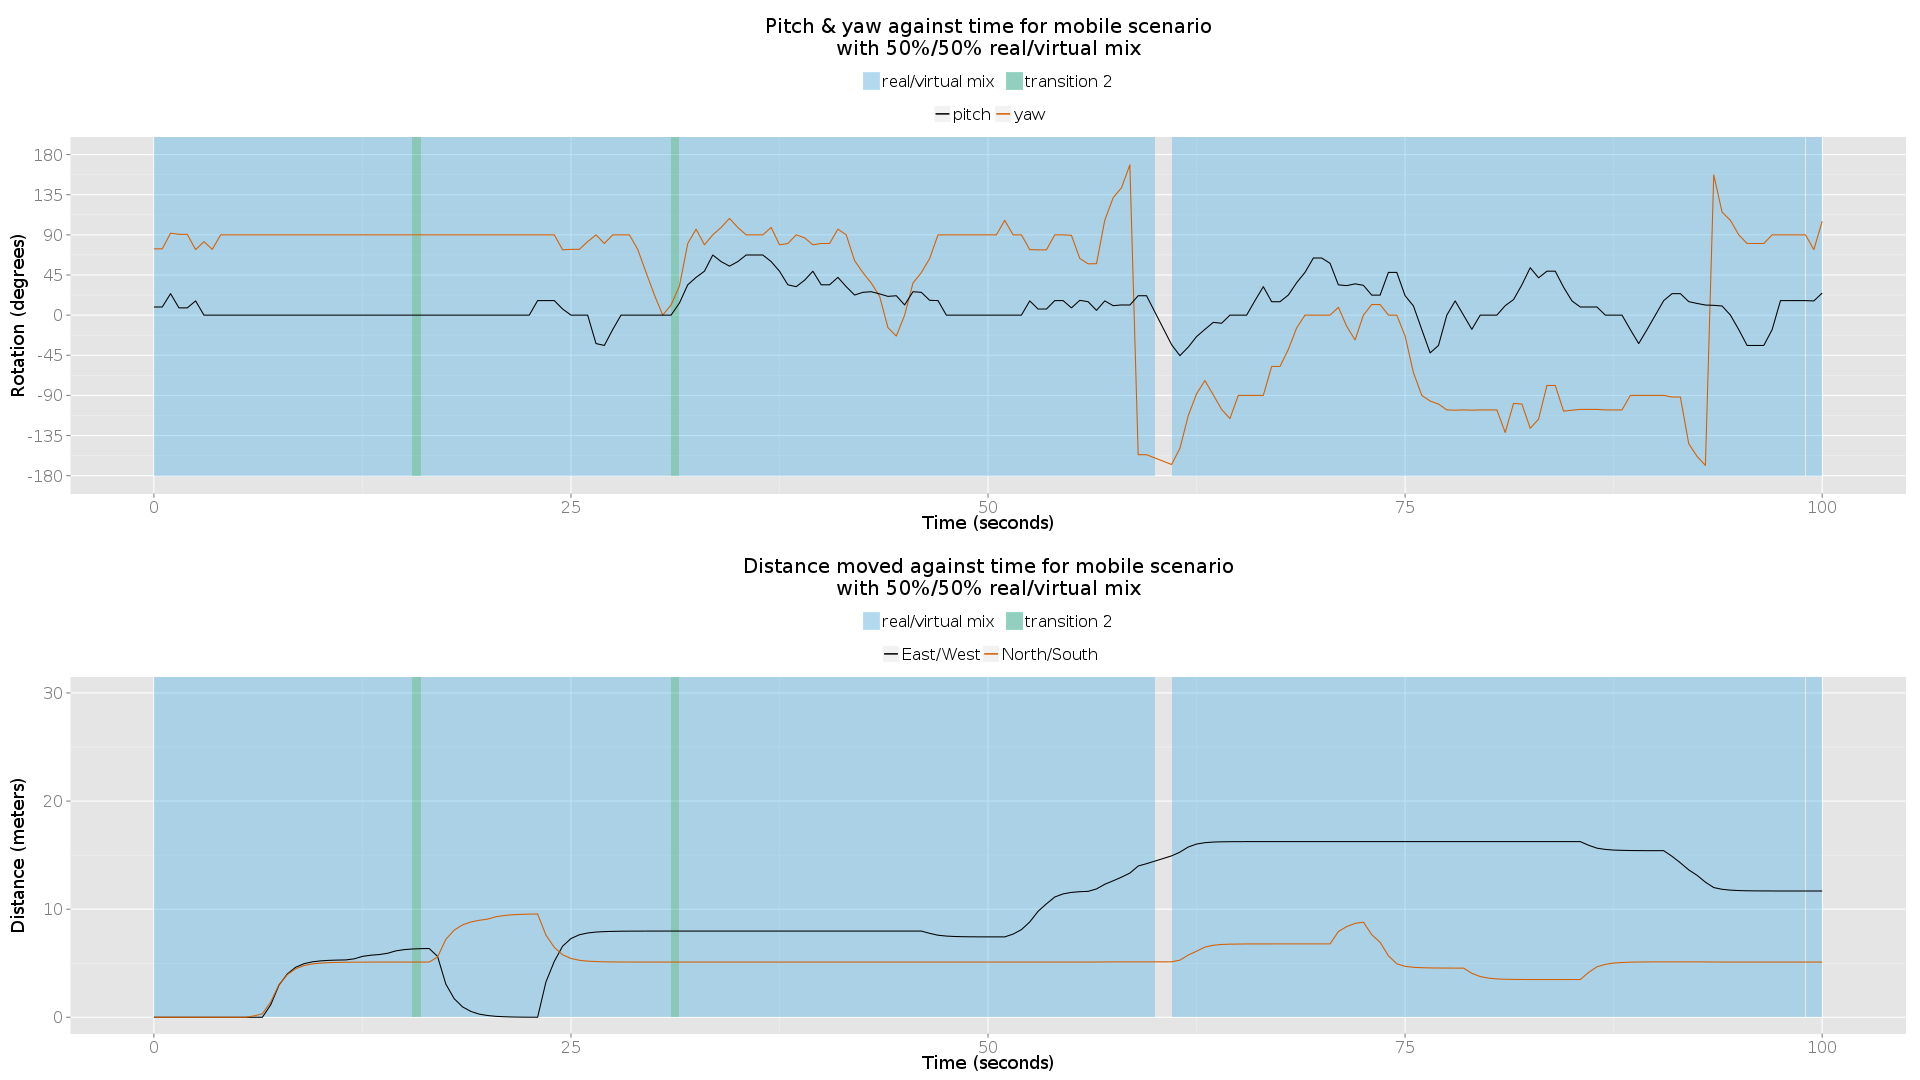
\includegraphics[width=\textwidth]{2.2/14_50_2up.png}
	\caption{Some images, yah.}
	\end{center}
\end{figure}

%=========================================================================================================

\clearpage

\subsubsection{Participant 15}

\begin{figure}[h]
	\begin{center}
	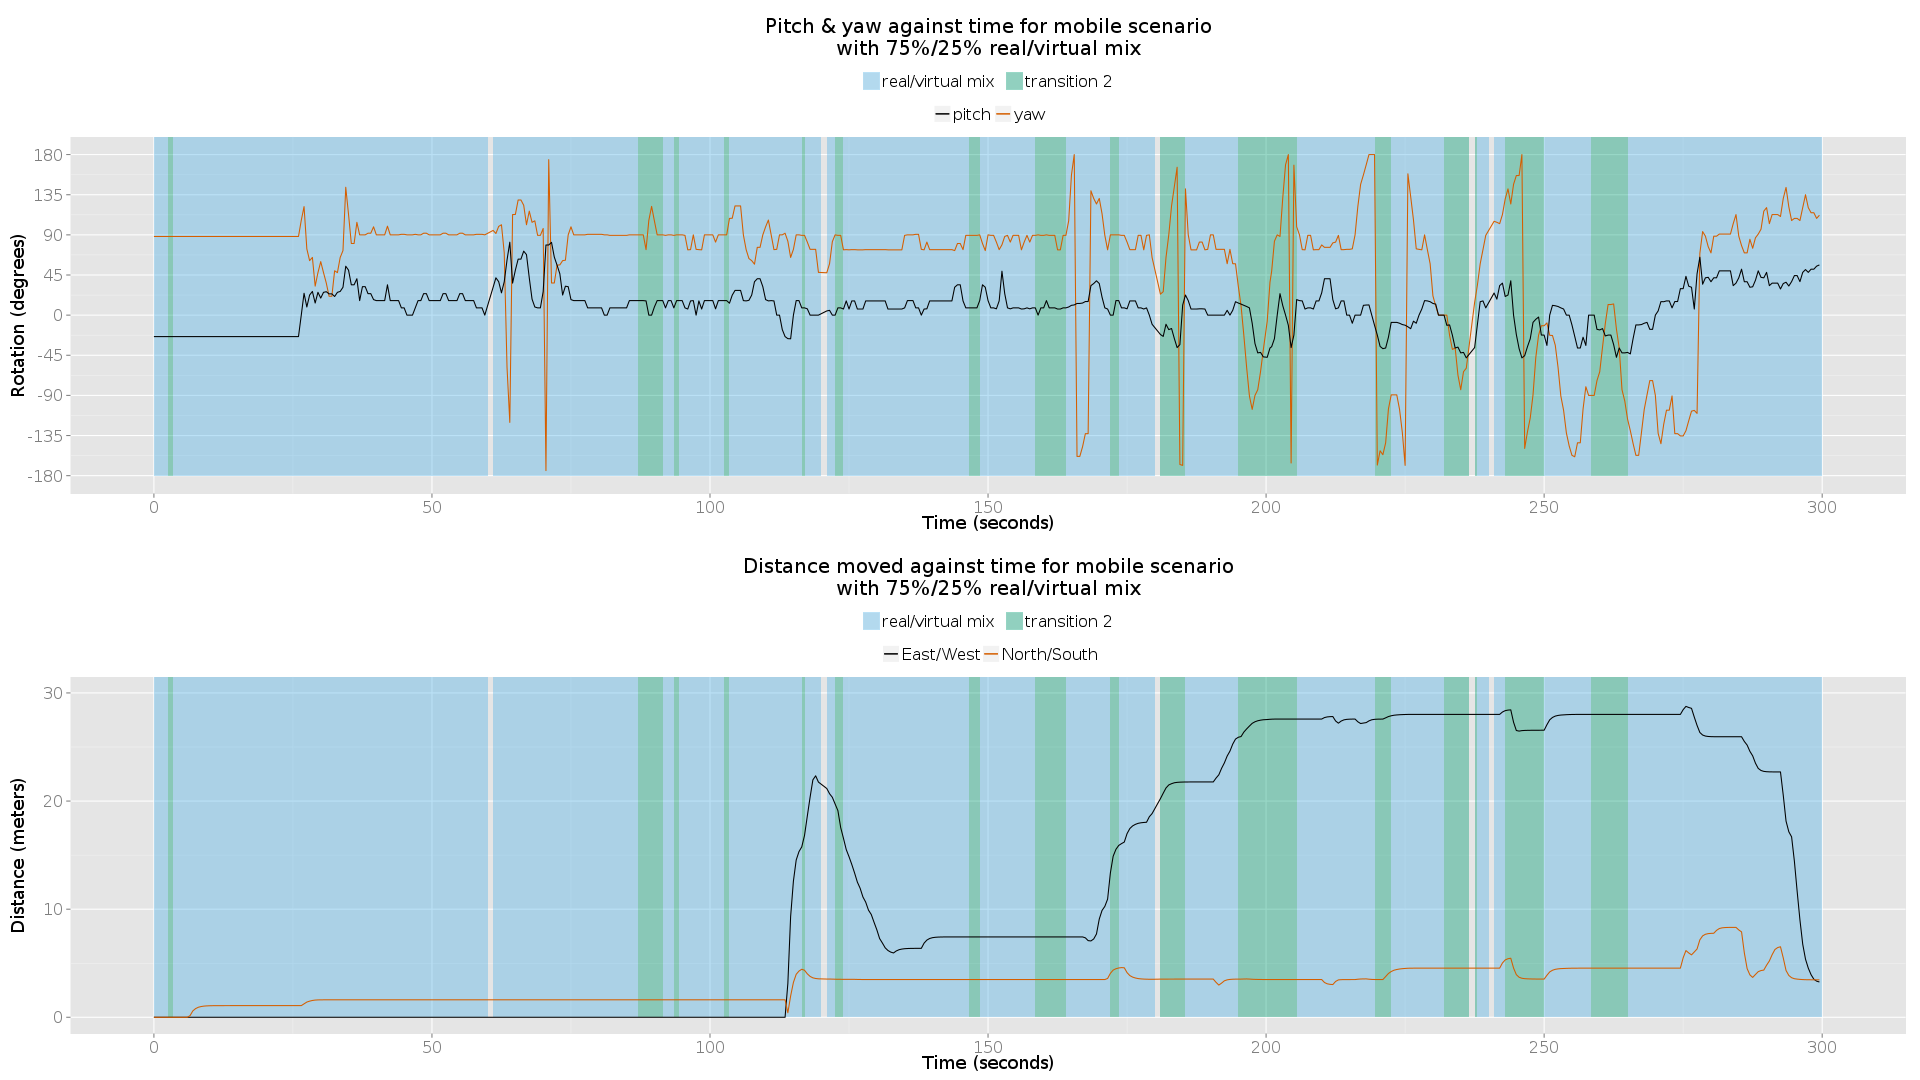
\includegraphics[width=\textwidth]{2.2/15_75_2up.png}
	\caption{Some images, yah.}
	\end{center}
\end{figure}

\clearpage

\begin{figure}[h]
	\begin{center}
	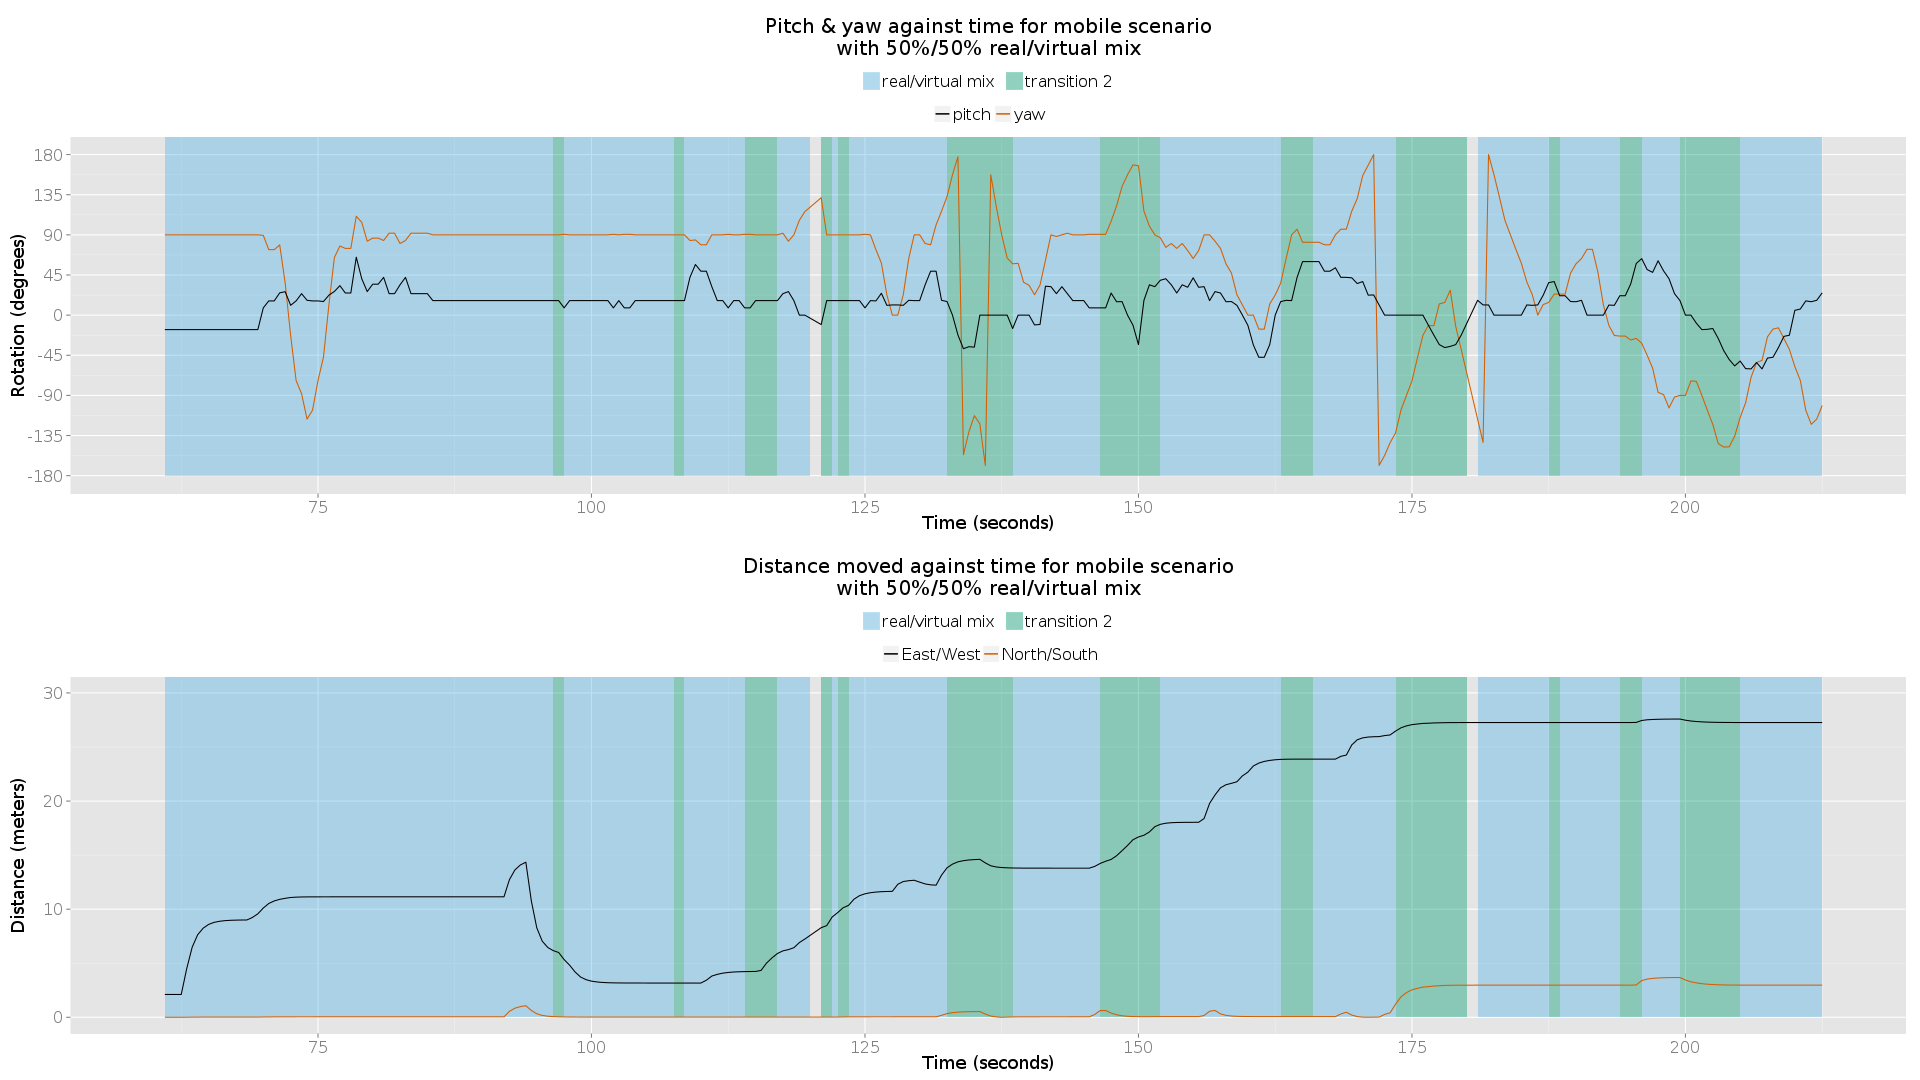
\includegraphics[width=\textwidth]{2.2/15_50_2up.png}
	\caption{Some images, yah.}
	\end{center}
\end{figure}

%=========================================================================================================

\clearpage

\subsubsection{Participant 16}

\begin{figure}[h]
	\begin{center}
	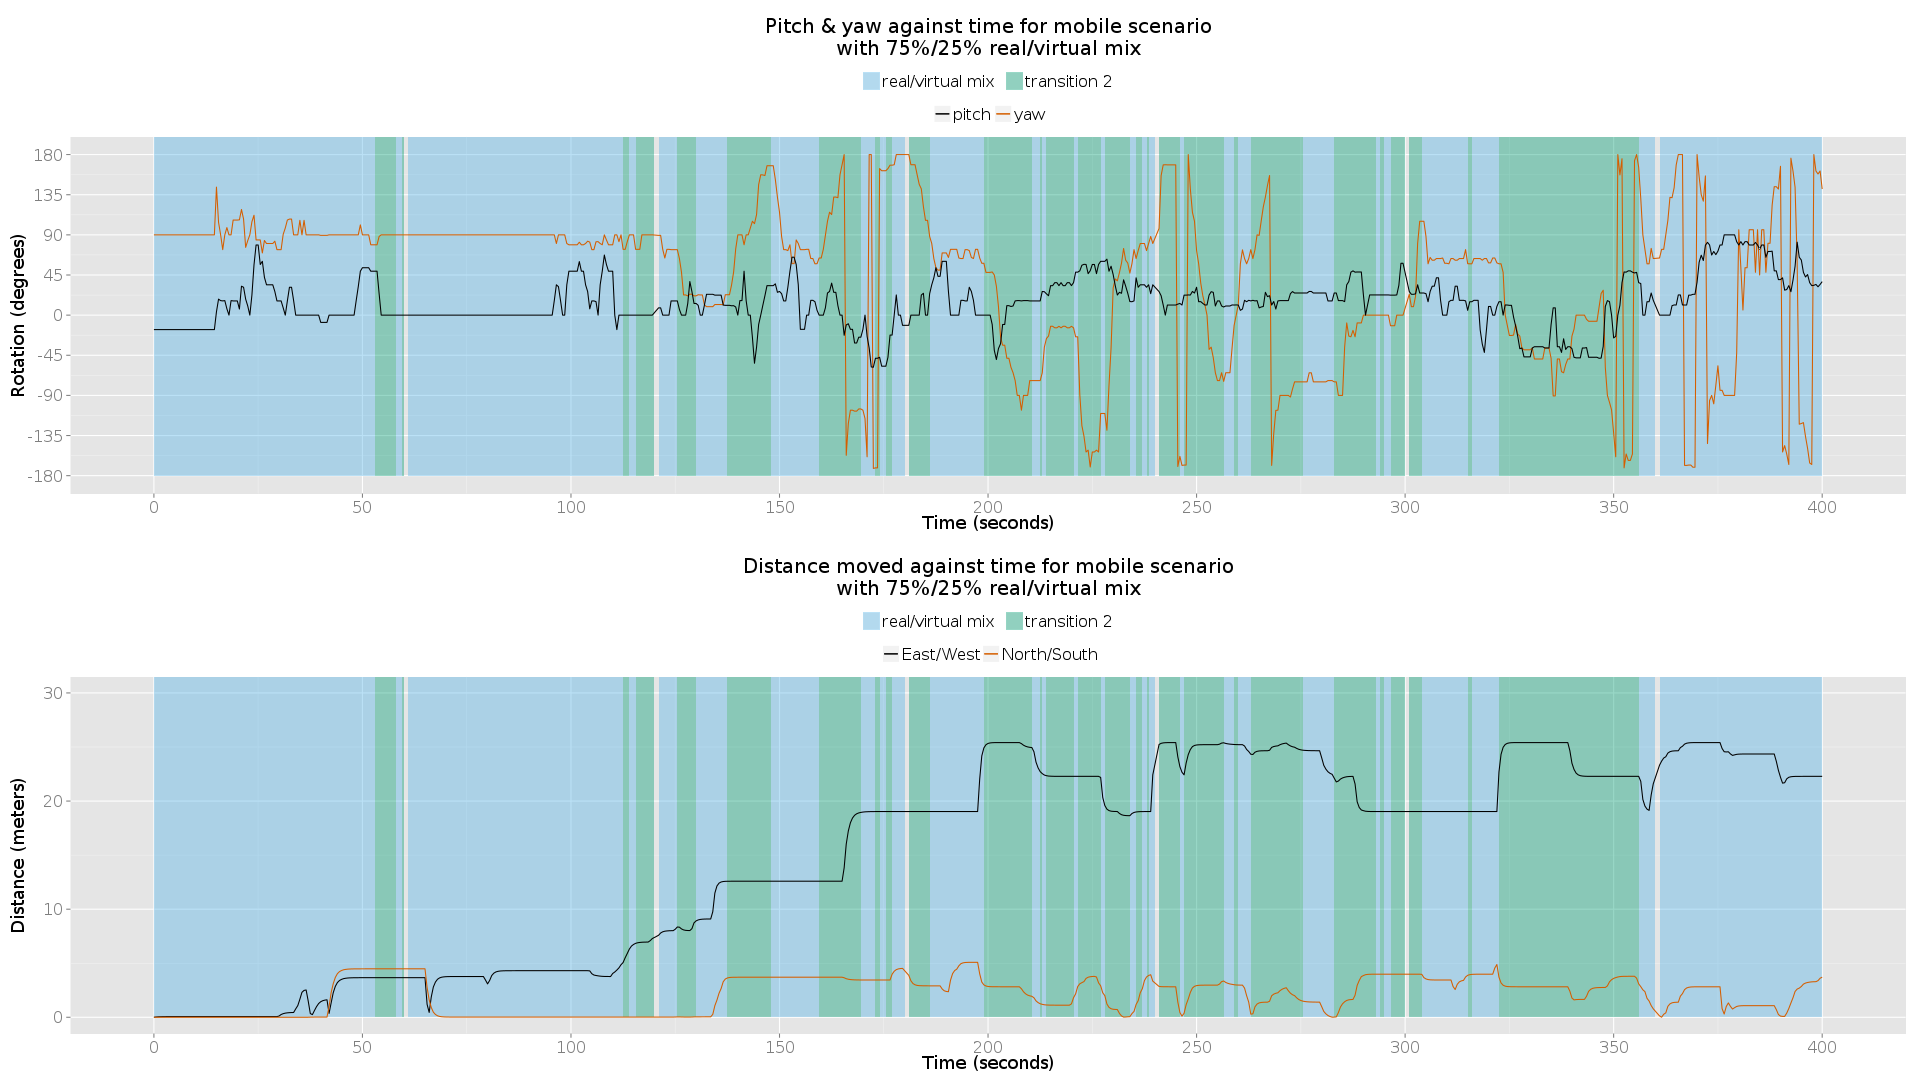
\includegraphics[width=\textwidth]{2.2/16_75_2up.png}
	\caption{Some images, yah.}
	\end{center}
\end{figure}

\clearpage

\begin{figure}[h]
	\begin{center}
	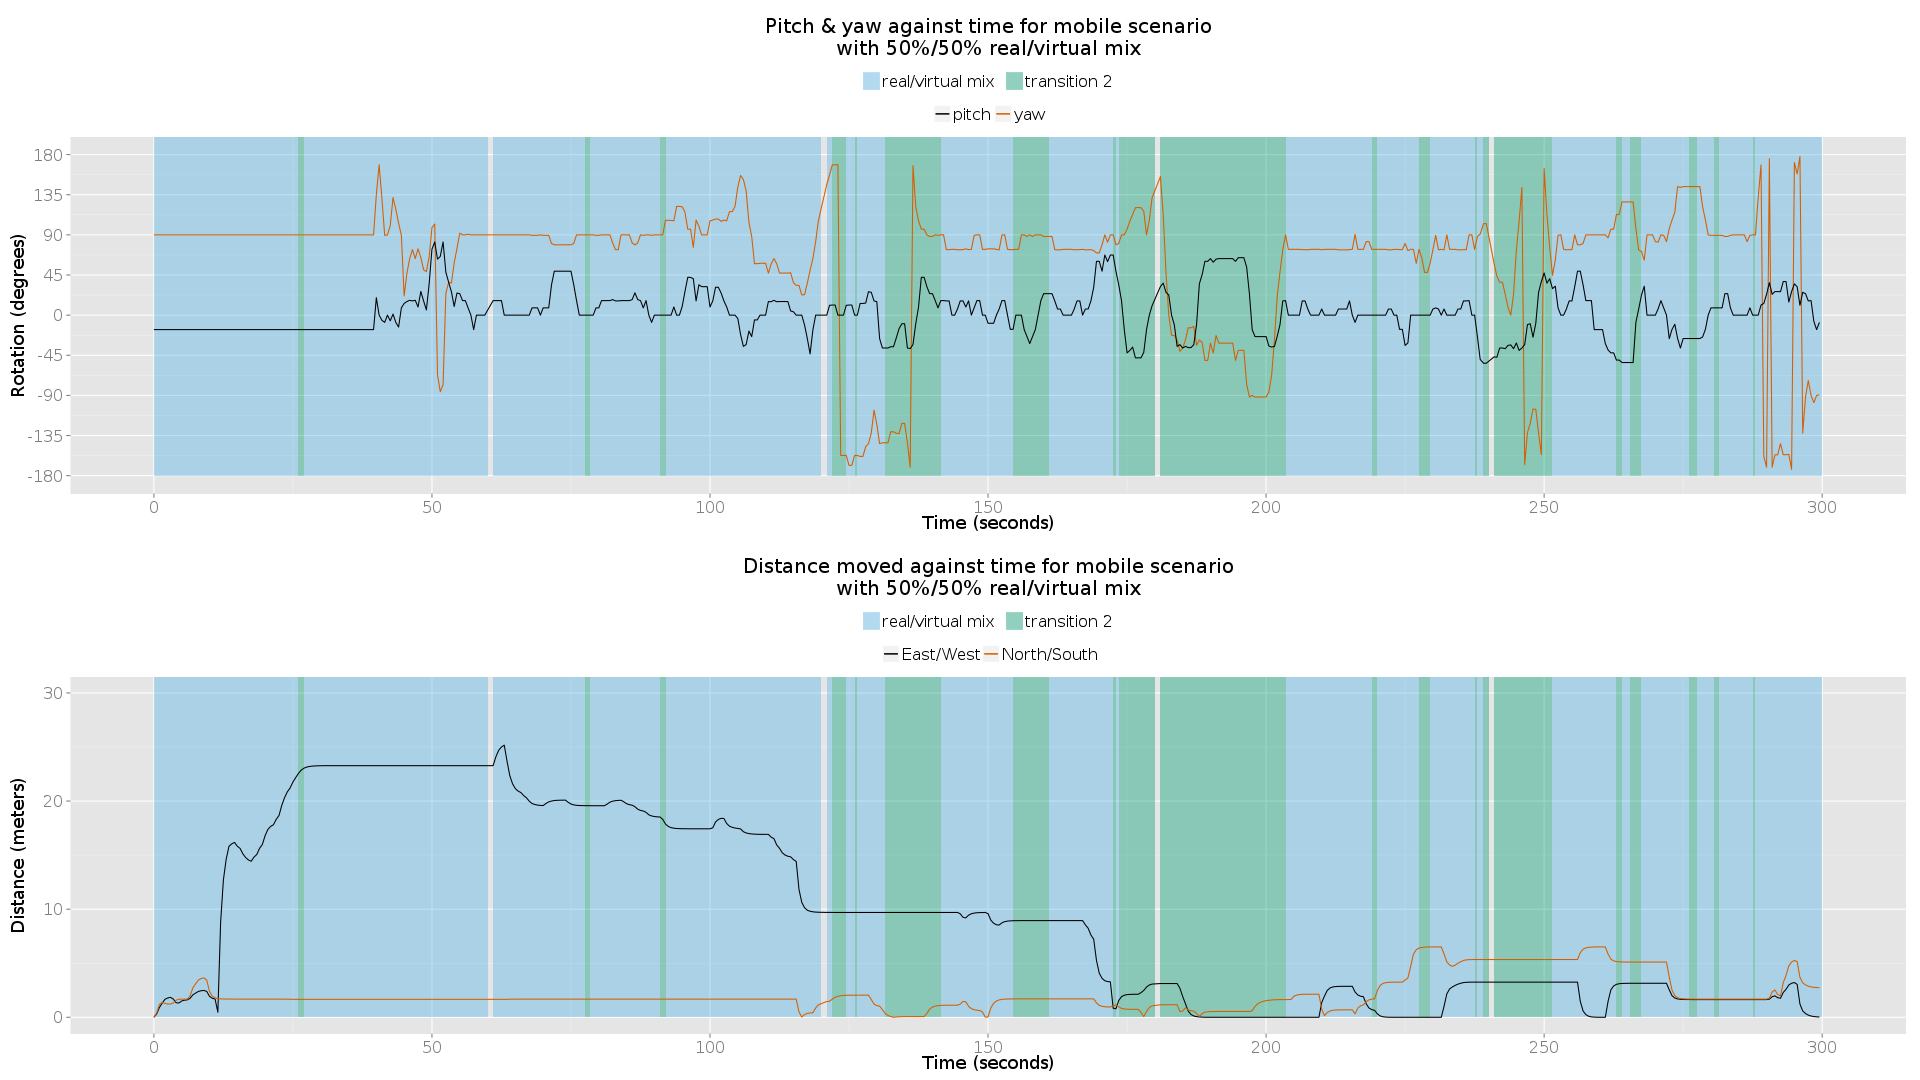
\includegraphics[width=\textwidth]{2.2/16_50_2up.png}
	\caption{Some images, yah.}
	\end{center}
\end{figure}

%=========================================================================================================

\clearpage

\subsubsection{Participant 17}

\begin{figure}[h]
	\begin{center}
	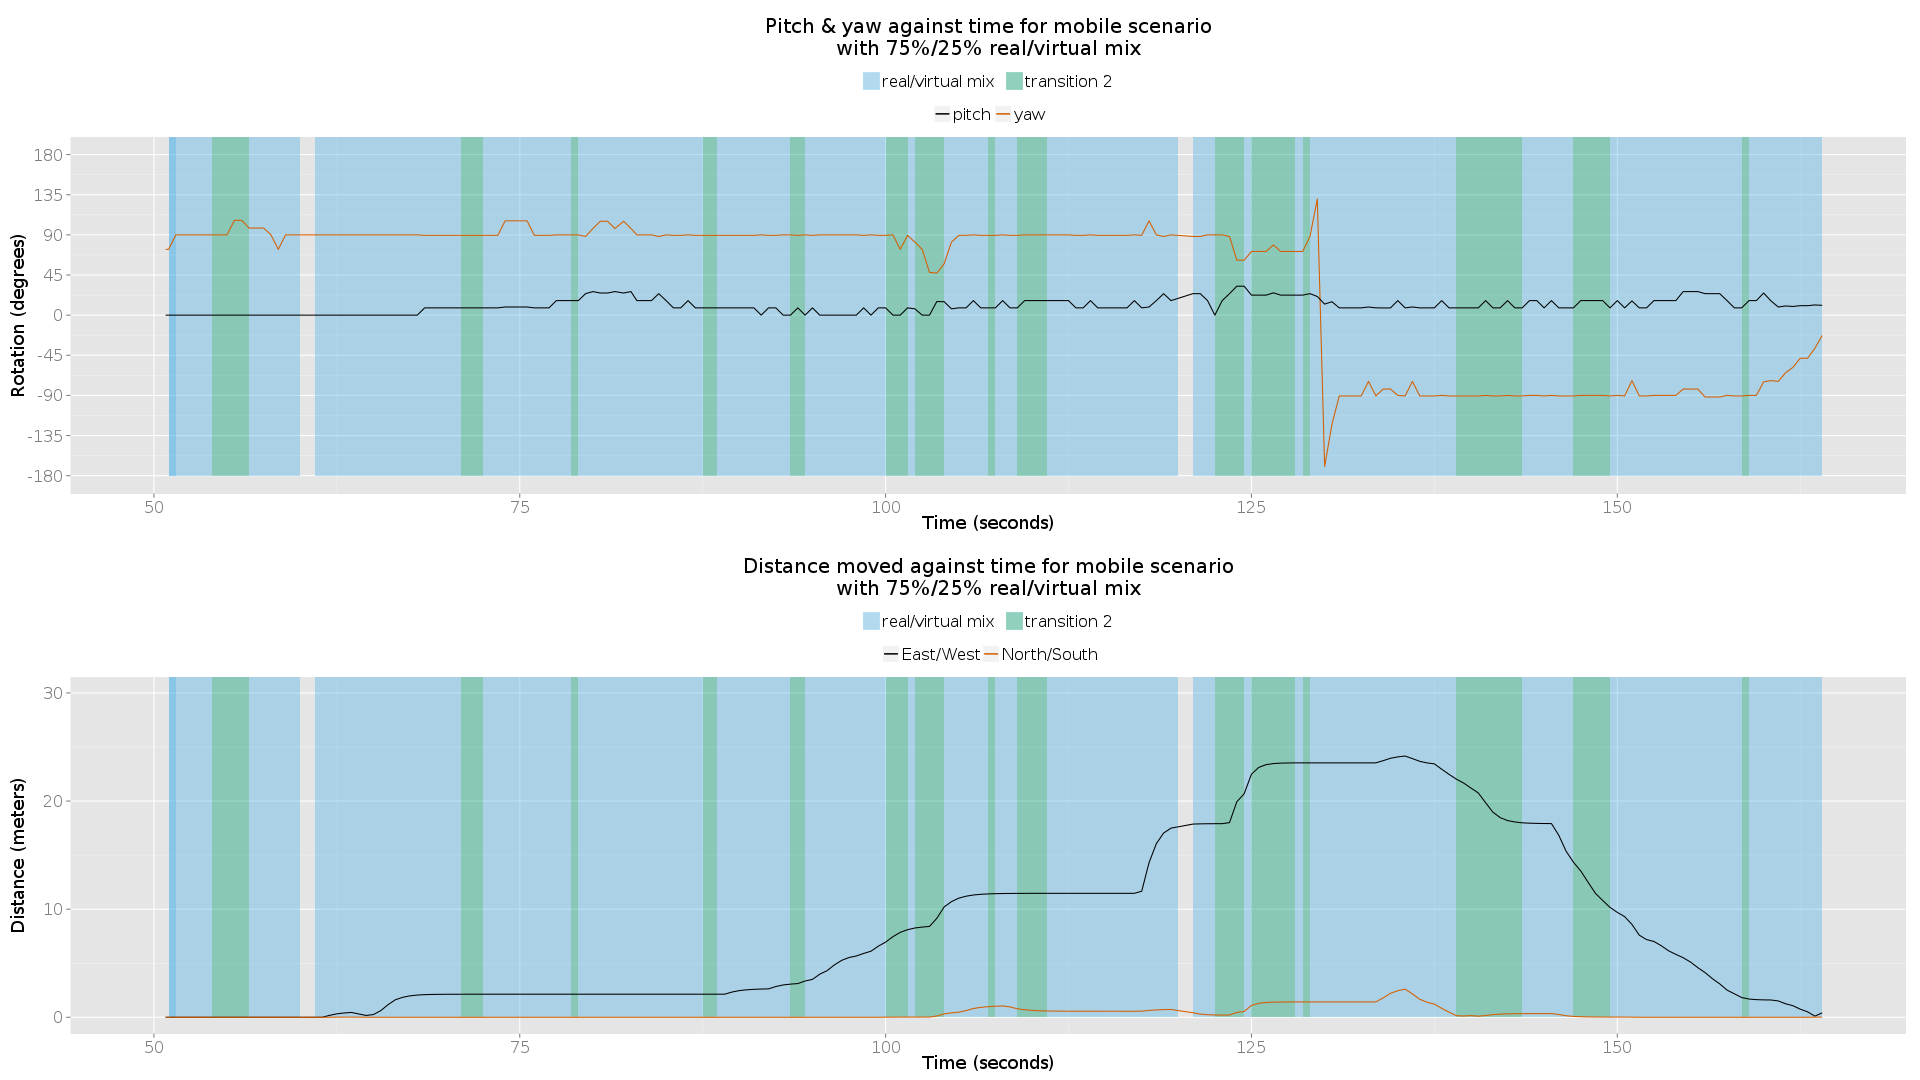
\includegraphics[width=\textwidth]{2.2/17_75_2up.png}
	\caption{Some images, yah.}
	\end{center}
\end{figure}

\clearpage

\begin{figure}[h]
	\begin{center}
	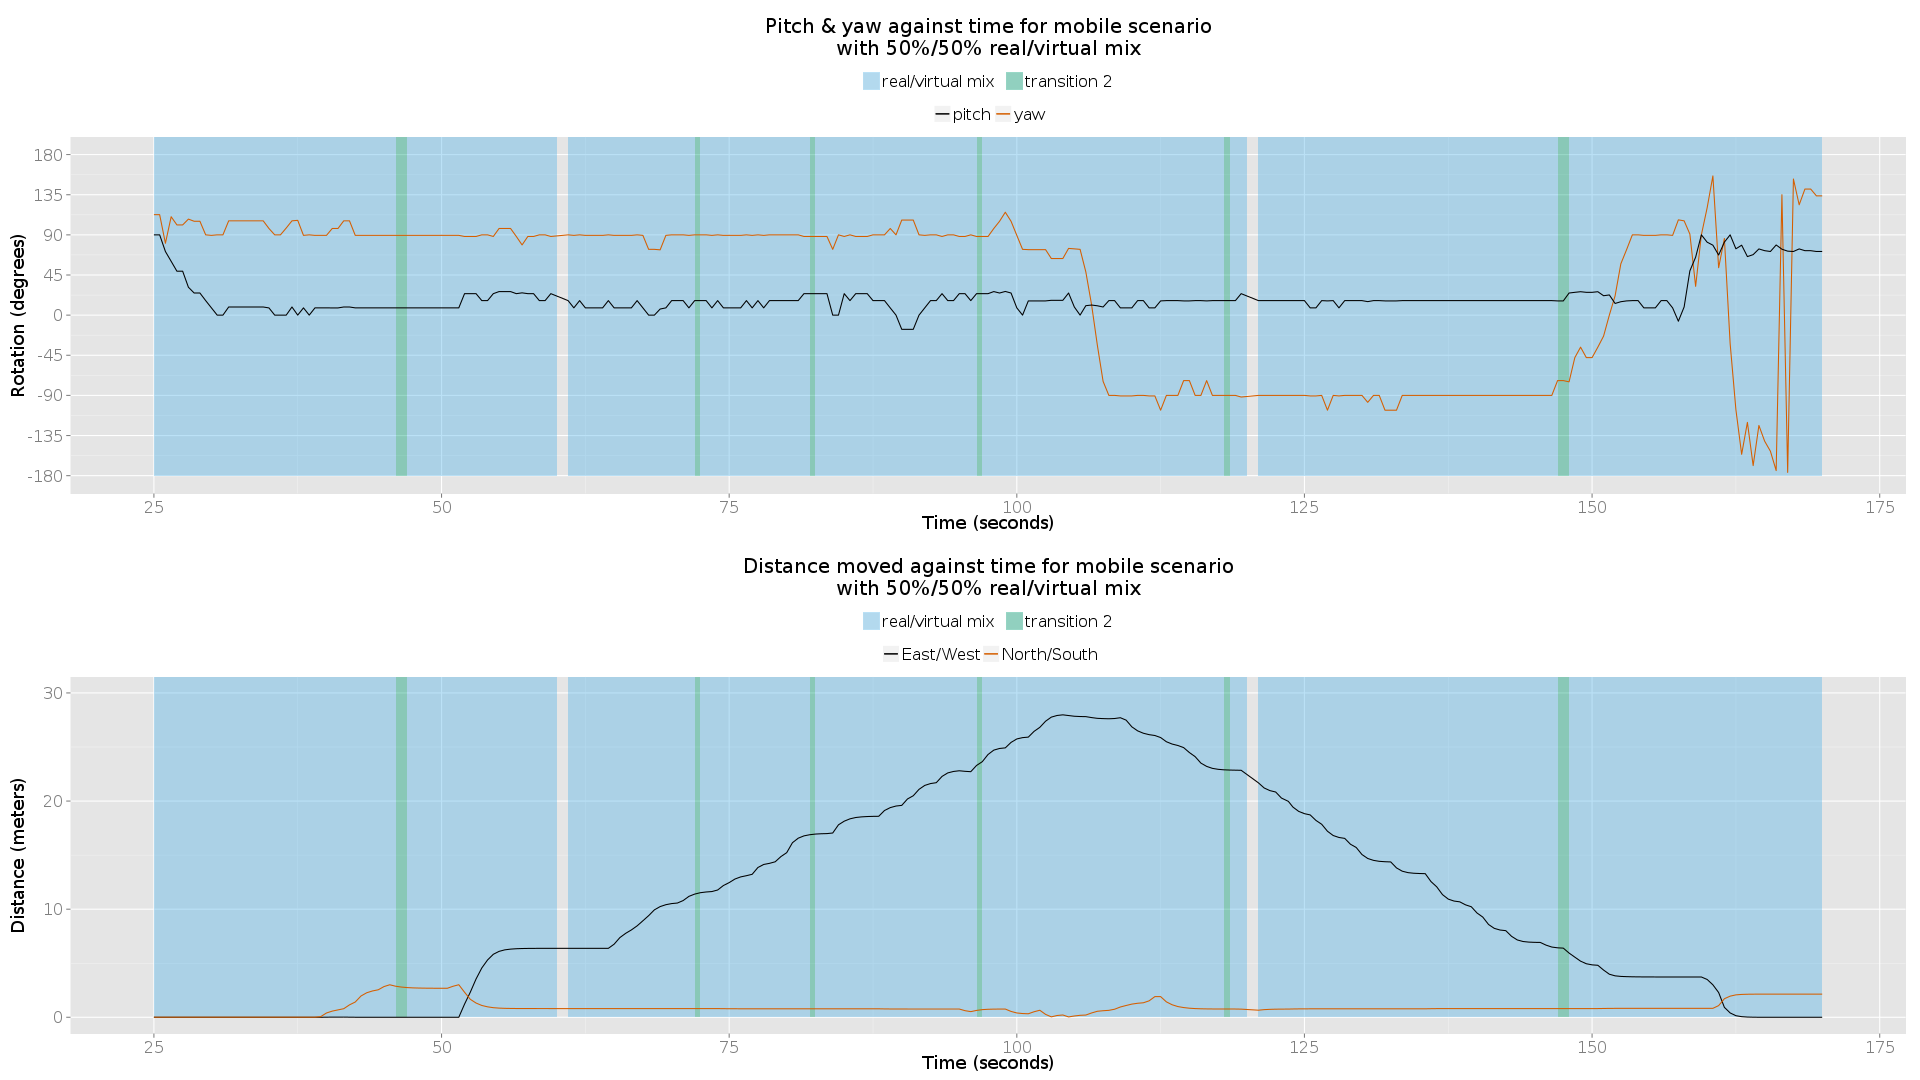
\includegraphics[width=\textwidth]{2.2/17_50_2up.png}
	\caption{Some images, yah.}
	\end{center}
\end{figure}

%=========================================================================================================

\section{Stage 2.2 Conclusions}

%=========================================================================================================

\section{Conclusions to Mirrorshades Evaluation Chapter}

%=========================================================================================================